\def \imgpath {"./figures/rt"}

In this chapter, measurements of \KOs, \LA, and \AL are reported as a function of underlying event activity classifiers \RT, \RTmin, and \RTmax. These observables quantify the magnitude of underlying event and are an experimental proxy of the \nmpi.

\section{Motivation for studying event sub-structure}

\subsection{Jet pedestal: underlying event}

As discussed in Chapter X, the underlying event, also known as jet pedestal in some literature, is composed of particles that are not directly related to the primary hard scattering and its related fragmentation. It can be studied to extract accurate information about the hard scattering process by subtracting it in precision measurements of jet properties. Moreover, since it is a manifestation of the proton substructure and the parton interactions, it can give us insight into the parton dynamics in the nonperturbative QCD region.

%In theory chapter, discuss UE history:
%J. R. Cudell et al., "Experimental study of the underlying event in high transverse momentum jet production at the CERN ISR", Nuclear Physics B, Volume 336, Issue 1, Pages 1-21 (1990). DOI: 10.1016/0550-3213(90)90568-V
%CDF Collaboration, "Observation of the Underlying Event in Dijet Events with a Leading Transverse Energy Jet at the Collider Detector at Fermilab", Physical Review Letters, Volume 83, Issue 7, Pages 1183-1188 (1999). DOI: 10.1103/PhysRevLett.83.1183
%DELPHI Collaboration, "Measurement of the underlying event in hadronic Z0 decays", Physics Letters B, Volume 382, Issues 3–4, Pages 323-332 (1996). DOI: 10.1016/0370-2693(96)00620-1

\subsection{Hard process--multiplicity bias}

Studying QGP phenomena in small systems as a function of event activity is challenging due to selection biases that arise when analyzing the data. It is known that selecting events with large momentum transfer leads to a bias towards higher multiplicities (and underlying event), and conversely, selecting events with higher multiplicities (and UE) enhances the hard processes. This bias can be understood in several ways. Firstly, a hard process tends to occur with lower impact parameters, which in turn leads to higher particle multiplicities. Secondly, an event with $n$ partonic interactions has $n$ chances of containing a hard process. Lastly, harder processes fragment into more particles, further contributing in higher event activity. As an example, Figure~\ref{fig:rt:hardbias} shows how the requirement of a high \pt track can skew the forward-rapidity centrality distribution to lower values (higher event activity), as observed in a result from ALICE.

\begin{figure}%
\subfloat[][]{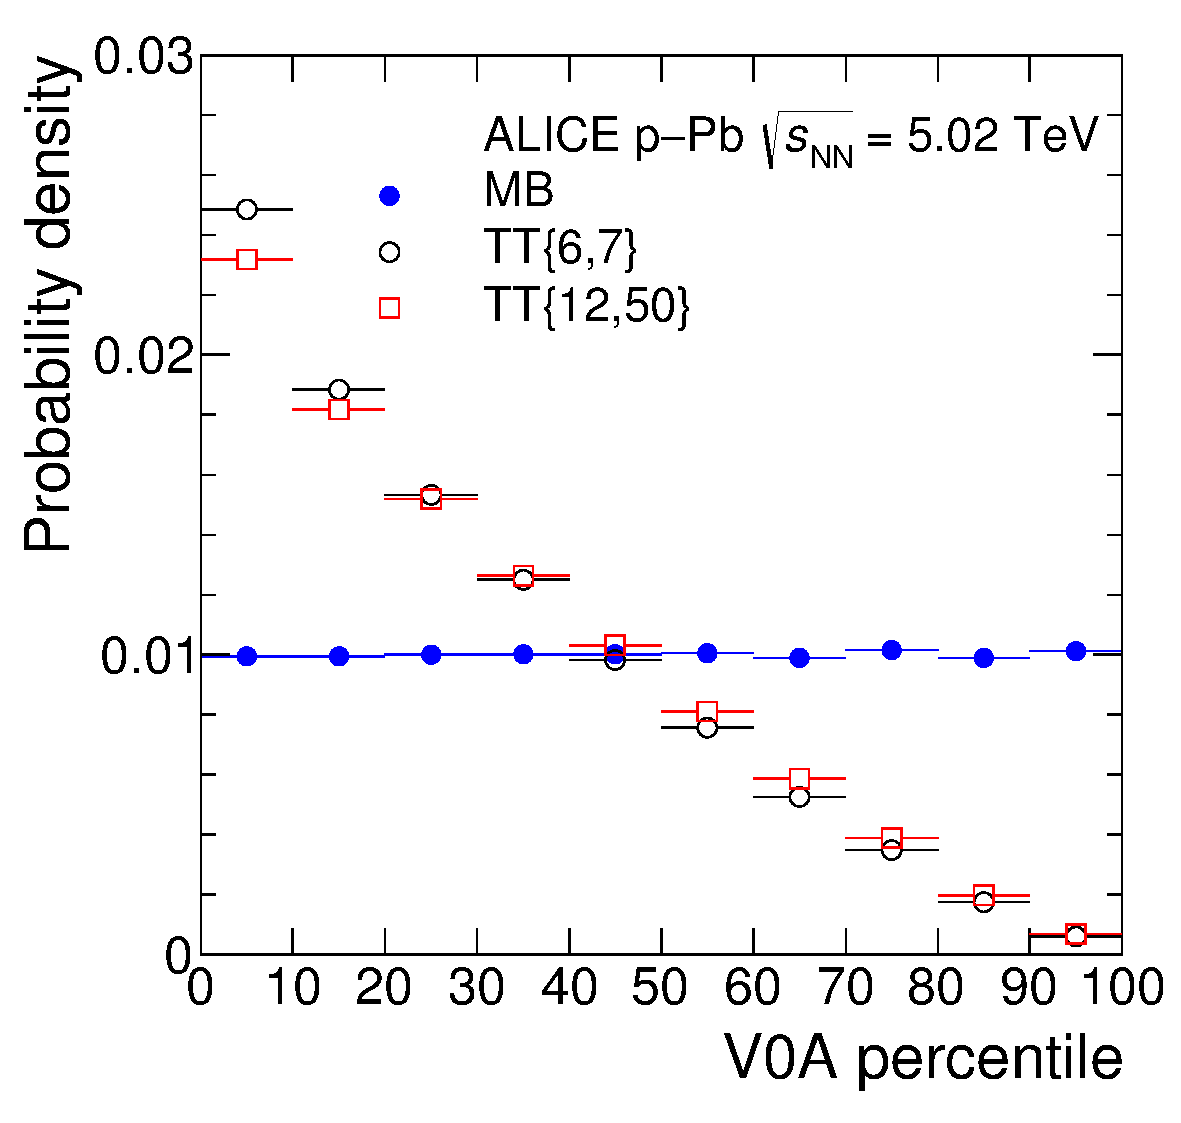
\includegraphics[width=.480\textwidth]{\imgpath/alice_hard_multi_bias.pdf}}\\
\caption{TBA}
\label{fig:rt:hardbias}
\end{figure}

\subsection{Azimuthal regions and transverse activity}

The selection bias of hard processes on UE becomes saturated at high \pt, where the impact parameter bias is fixed and stochastic effects become comparable. This saturation effect can be observed when studying particle production in three topological regions defined with respect to the highest momentum track, which serves as a proxy for the axis of the primary scattering process. The three regions are defined as follows:
\begin{enumerate}
\item Towards (also known as "Near"), where $|\phi - \philead| < \frac{\pi}{3}$,
\item Away, where $|\phi - \philead| > \frac{2\pi}{3}$, and 
\item Transverse, where $\frac{\pi}{3} < |\phi - \philead| < \frac{2\pi}{3}$. 
\end{enumerate}
Here, \philead is the azimuthal angle of the leading track. This definition is illustrated in Figure~\ref{fig:rt:rtdefi}. 

\begin{figure}%
\subfloat[][]{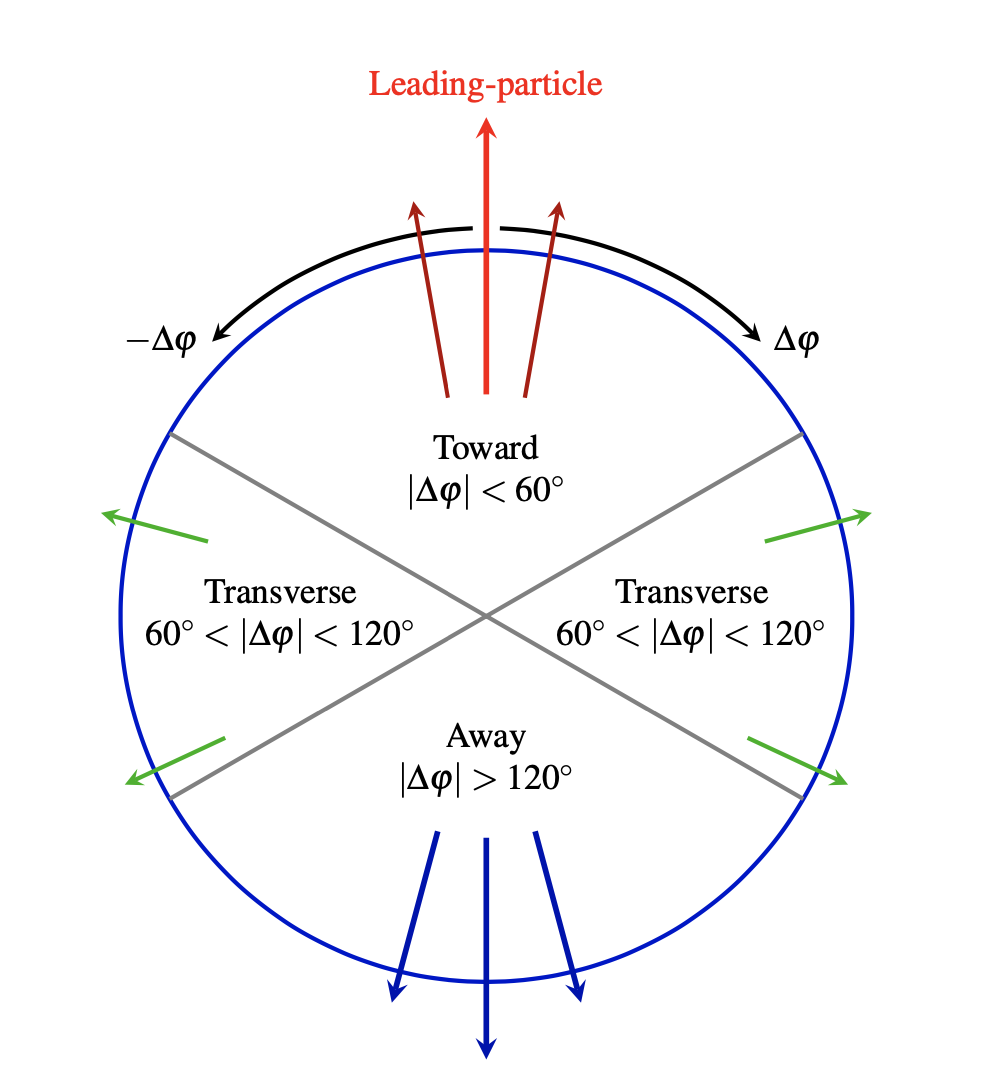
\includegraphics[width=.490\textwidth]{\imgpath/rt_defi.png}}
\subfloat[][]{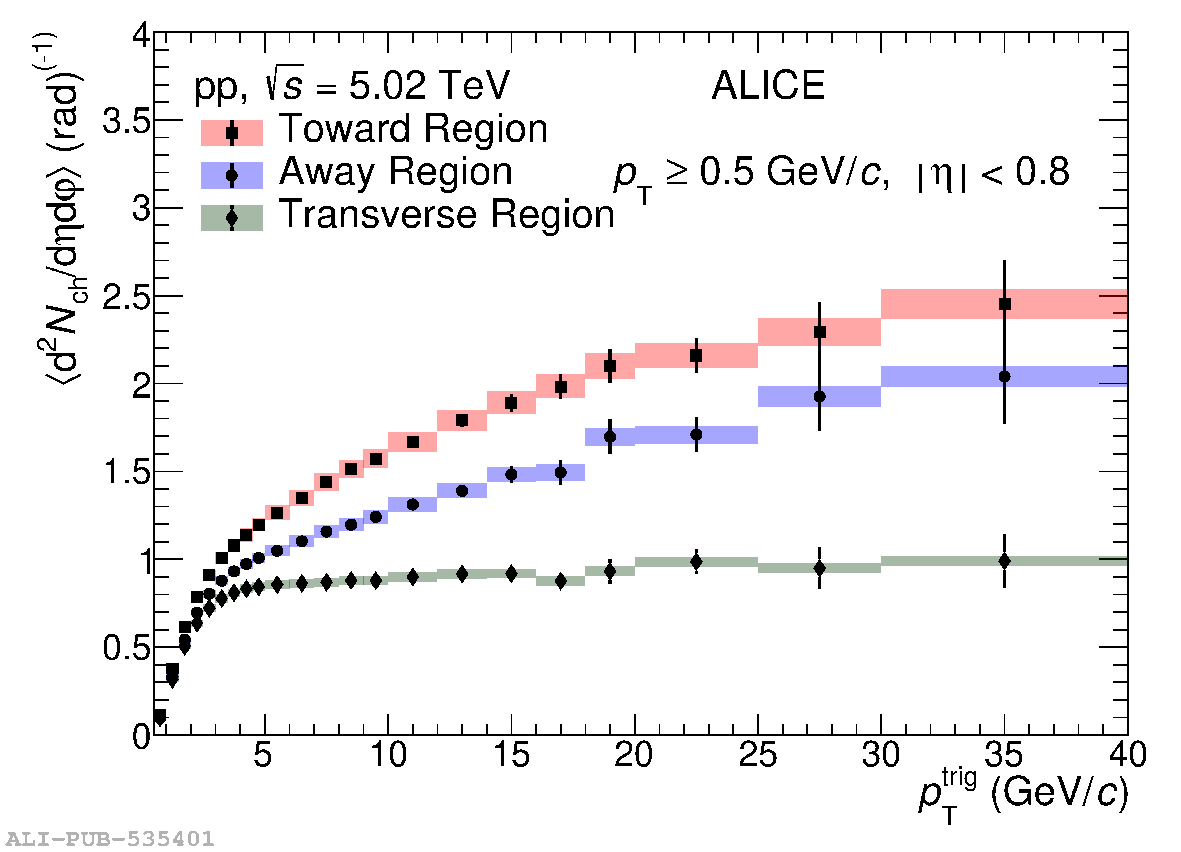
\includegraphics[width=.490\textwidth]{\imgpath/alice_uevpt.pdf}}\\
\caption{TBA}
\label{fig:rt:rtdefi}
\end{figure}

Studying particle multiplicity (or sum of their \pt) in these regions as a function of the transverse momentum of the leading track \ptlead reveals that in the regions Towards and Away, the multiplicity continues to increase with the hardness of the primary process. These regions contain the leading and the recoil jet, respectively. In contrast, in the Transverse region, the multiplicity (further denoted as $N_T$ in this thesis but $N_\mathrm{ch}^\mathrm{trans}$ is also used in cited literature) reaches a plateau at around $\gevc{5}$. In this region, the underlying event becomes independent of the strength of the primary process, and the selection bias is minimized. Notably, this phenomenon is universal regardless of the system size or collision energy. As an example, measurements from ALICE are shown in Fig.~\ref{fig:rt:rtdefi}.

\section{\RT as an experimental observable}

The magnitude of the underlying event can be measured using the self-normalized ratio:
\begin{align}
\RT = \frac{N_T}{\langle N_T \rangle},
\end{align}
which is often referred to as the underlying event activity, transverse activity, or relative transverse activity in various literature, and also in this thesis. This observable and its uses were suggested in Ref.~\cite{skands-rt}.

By applying $\RT$, two limits of events can be studied:
\begin{itemize}
\item $\RT \rightarrow 0$: the \textbf{``ee"} limit, where events with minimal UE are selected. These events are dominated by a single hard scattering and can be compared to LEP fragmentation models.
\item $\RT \rightarrow \infty$: the \textbf{``AA"} limit, where events with very high transverse activity are selected, which can come from many MPIs and/or from transverse jets. These events may exhibit collective features similar to AA collisions.
\end{itemize}

\subsection{Proxy to \nmpi}

As could be intuitively expected, \RT serves as an experimental proxy for \meannmpi. Phenomenological models that incorporate MPIs provide an illustration of this relationship. As shown in Fig.~\ref{fig:rt:nmpi}, Pythia 8 predicts a strong dependence of \meannmpi on \RT until $\RT \lesssim 5$. Similarly, Herwig 7 predicts a dependence until $\RT \lesssim 3$, albeit weaker. Pythia's prediction for the relationship between \RT and the event multiplicity, which is affine, is also shown in the figure.

\begin{figure}%
\subfloat[][]{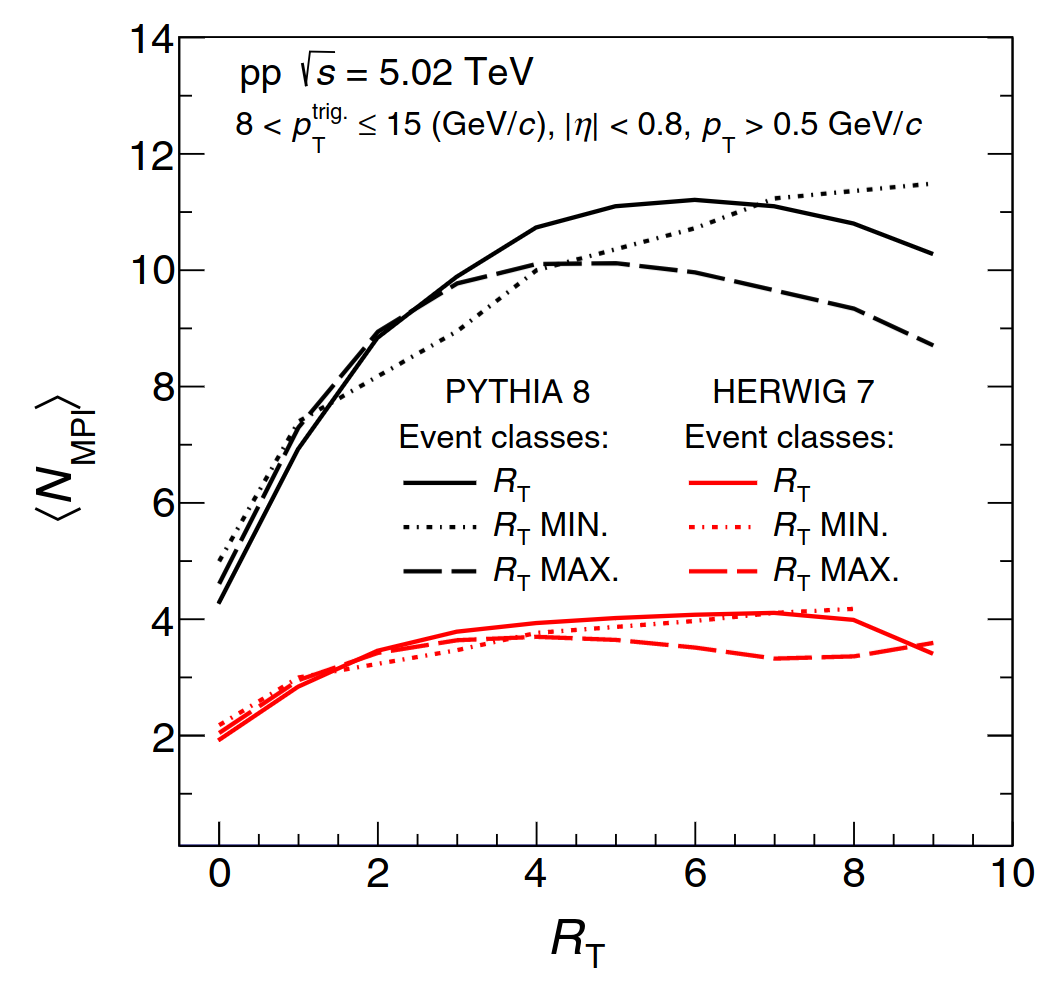
\includegraphics[width=.480\textwidth]{\imgpath/rt_minmax_nmpi.png}}
\subfloat[][]{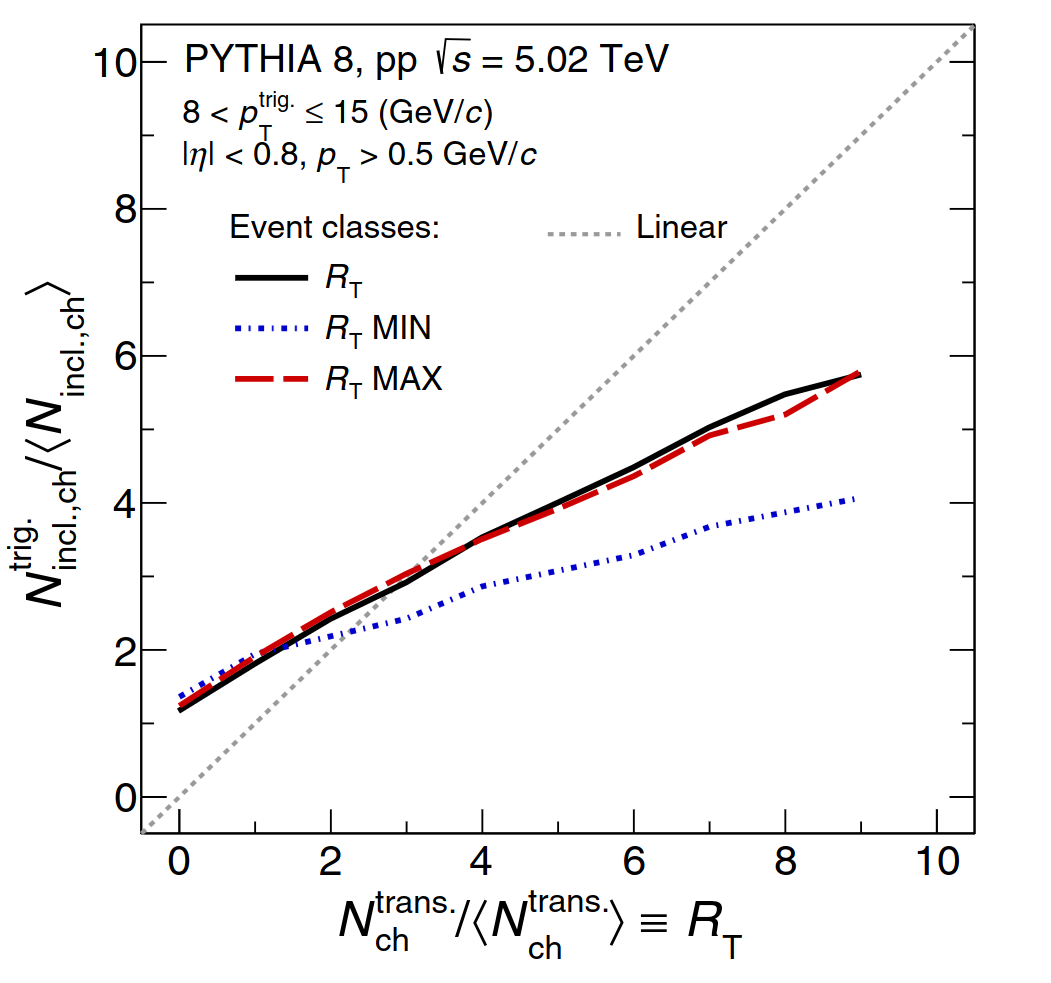
\includegraphics[width=.465\textwidth]{\imgpath/rt_nch.png}}\\
\caption{TBA}
\label{fig:rt:nmpi}
\end{figure}


\subsection{Extension to \RTmin, \RTmax}

To separate the soft and hard components of the underlying event -- namely, the MPIs from ISR/FSR -- the definition of \RT can be extended. The two transverse sub-regions can be further classified as Transverse-min or Transverse-max, based on which sub-region has fewer or more particles. Softer contributions from MPIs will enter both sub-regions, whereas the effects of harder radiation should be captured in the Transverse-max sub-region. This makes Transverse-min more sensitive to particle production from MPIs.

Analogously, the following underlying event activity classifiers can be defined:
\begin{align}
\RTmin &= \frac{\NTmin}{\langle \NTmin \rangle} \quad, \\
\RTmax &= \frac{\NTmax}{\langle \NTmax \rangle} \quad,
\end{align}
where \NTmin and \NTmax are the particle multiplicities in the Transverse-min and Transverse-max sub-regions, respectively. This approach follows measurements developed at UE studies at Tevatron and have been suggested to use in searches for QGP phenomena in small systems based on investigations in phenomenological models \cite{antonio-rtmin}.

According to Pythia 8, as shown in Fig.~\ref{fig:rt:nmpi}, \RTmin and \RTmax follow different relationships with \meannmpi. Whereas \meannmpi starts falling as a function of \RTmax (due to the inclusion of mini-jets) at $\RTmax \approx 5$, it continues rising as a function of \RTmin across the entire range. Furthermore, compared to \RT, \RTmin also shows some degree of decorrelation with event multiplicity.


\subsubsection{Charged particle \pt spectra}

Phenomenological models also reveal a significantly different evolution of transverse momentum spectra of inclusive charged particles based on \RTmin and \RTmax, as shown in Fig.~\ref{fig:rt:nchpt}. For the highest reported ranges of \RTmax and \RT, a significant hardening of the spectrum is observed in both Pythia 8 and Herwig 7, similarly to multiplicity studies \cite{alice-lfsmallsystems}, indicating a strong auto-correlation. In contrast, \RTmin exhibits a Cronin-like enhancement at intermediate \pt and a plateau at $\pt \gtrsim \gevc{6}$, even in the highest \RTmin bin. 

\begin{figure}%
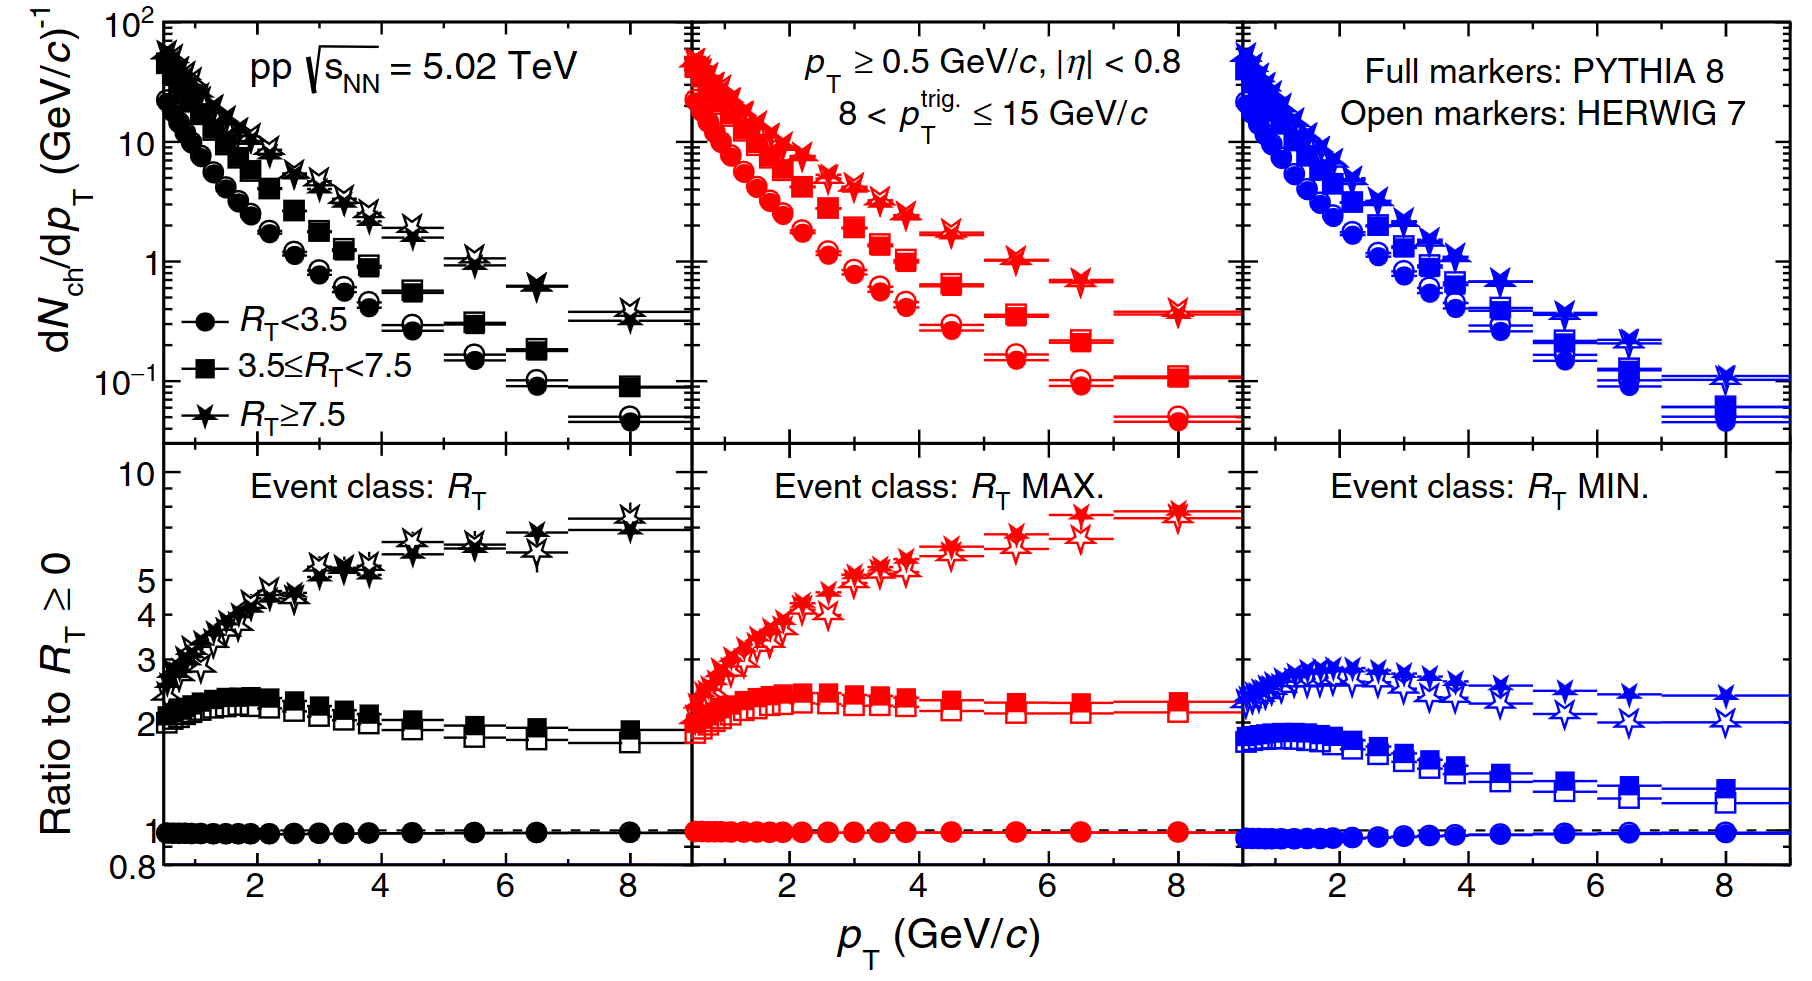
\includegraphics[width=.980\textwidth]{\imgpath/rt_nchpt.png}
\caption{TBA}
\label{fig:rt:nchpt}
\end{figure}

\subsection{Track and event selection}

%\subsection{\RT}

The event selection follows the same criteria as the \SOPT measurement discussed in Section~\ref{sec:sphero:eventtracks}, which conform to the standard analysis of light flavour hadrons versus multiplicity in pp collisions conducted in ALICE. The \INELgtO events, which require at least one hit in either \VOA or \VOC scintillators and a track reconstructed within $|\eta|<1$, are used. The SPD is used for the reconstruction of primary vertex, which is further required to have $|\Delta z|<10$~cm to reject out-of-bunch pile-up. To remove in-bunch pile-up, events with multiple reconstructed vertices are excluded.

Events are required to have a leading track with reconstructed momentum $5 < \ptlead < \gevc{40}$\footnote{Note that \pt spectrum is falling very steeply, at an approximately exponential rate, making the upper bound negligibly restrictive compared to the lower bound.}. These values were chosen to access the plateau in transverse activity and isolate the UE while retaining a large data sample. Maintaining a high momentum and spatial resolution of the leading track is crucial in this measurement. However, this can be compromised at high \pt when a significant portion of the track curvature can fall between two sectors of the TPC. To address this issue, geometrical cuts are used, as discussed in Section~\ref{TBA}.

For both the leading particle as well as the particles entering \NT and \RT calculations, tracks are required to be within $|\eta|<0.8$ and have $\pt > \gevc{0.15}$, and must satisfy the following:
\begin{enumerate}
\item ``Hybrid tracks", described in more detail in Section~\ref{TBA}, are used for both leading and \NT tracks to ensure a high level of azimuthal acceptance uniformity. These tracks consist of high-quality ``global track" requirements, including the SPD information, which leads to azimuthal non-uniformity, and ``complementary track" cuts, a looser set requiring only ITS and TPC in cases where the first are not satisfied.
\item  For the leading track, strict \pt-dependent DCA cuts are applied in the transverse direction ($|\mathrm{DCA}_{xy}| < 0.0182 + \frac{0.0350}{\pt^{1.01}}$~cm, $\pt \in [ \mathrm{\gevc} ]$), to ensure good momentum resolution and that the track is a primary one.
\item For the \NT tracks, a DCA cut ($|\mathrm{DCA}_{xy}| < 0.06$~cm) is required to avoid biases in \VO measurements, as explained in the text below.
\end{enumerate}

\subsection{\RT measurements of neutral particles vs. charged particles}

The \VOs are neutral particles and thus, they cannot be leading tracks nor enter \NT (\NTmin, \NTmax) and \RT (\RTmin, \RTmax) calculations. This has several implications:
\begin{enumerate}
\item \VOs suffer much less from auto-correlation biases than \pikp, which can be seen in azimuthal distributions and in $\KOs / \mathrm{K}^\pm$ ratios. Requiring high/low \NT/\RT can lead to an increase/decrease of charged particles in the Transverse region due to selecting fluctuations in addition to the UE scaling. However, this effect is significantly smaller for neutral \VOs. This behaviour is shown in Fig.~\ref{fig:rt:autocorr}. It is important to bear this caveat in mind when comparing \pt spectra and yields of \pikp and \VOs.
\item While \NT is always at least $1$ for \pikp in the Transverse region, for \VOs it can be equal to $0$. Similar logic applies to the Transverse-min/max sub-regions and \NTmin/\NTmax .
\item The maximum \pt measurable for \pikp in the Toward region is limited to $\pt < \gevc{5}$, where the trigger requirement leads to a trivial increase. For \VOs, however, this limitation does not apply and their measured \pt range does not need to be restricted.
\item The charged daughters of \VOs could sometimes enter \NT, leading to significant biases at low \pt in the Toward and Away regions of $\KOs/\mathrm{K}^\pm$ ratios. 
\end{enumerate} 

In this thesis, the behaviour described in the last point was rectified by making \NT track candidates and \VO daughter tracks two disjunct sets. This was achieved by applying the $|\mathrm{DCA}_{xy}|>0.06$~cm cut, used in the \VO reconstruction as discussed in Section~\ref{sec:ana:cuts}, in opposite ways. This reduces the \NT track candidates by less than $5\%$. The effect of this solution can be seen in Fig.~\ref{fig:rt:KtoK}.

\begin{figure}%
\subfloat[][]{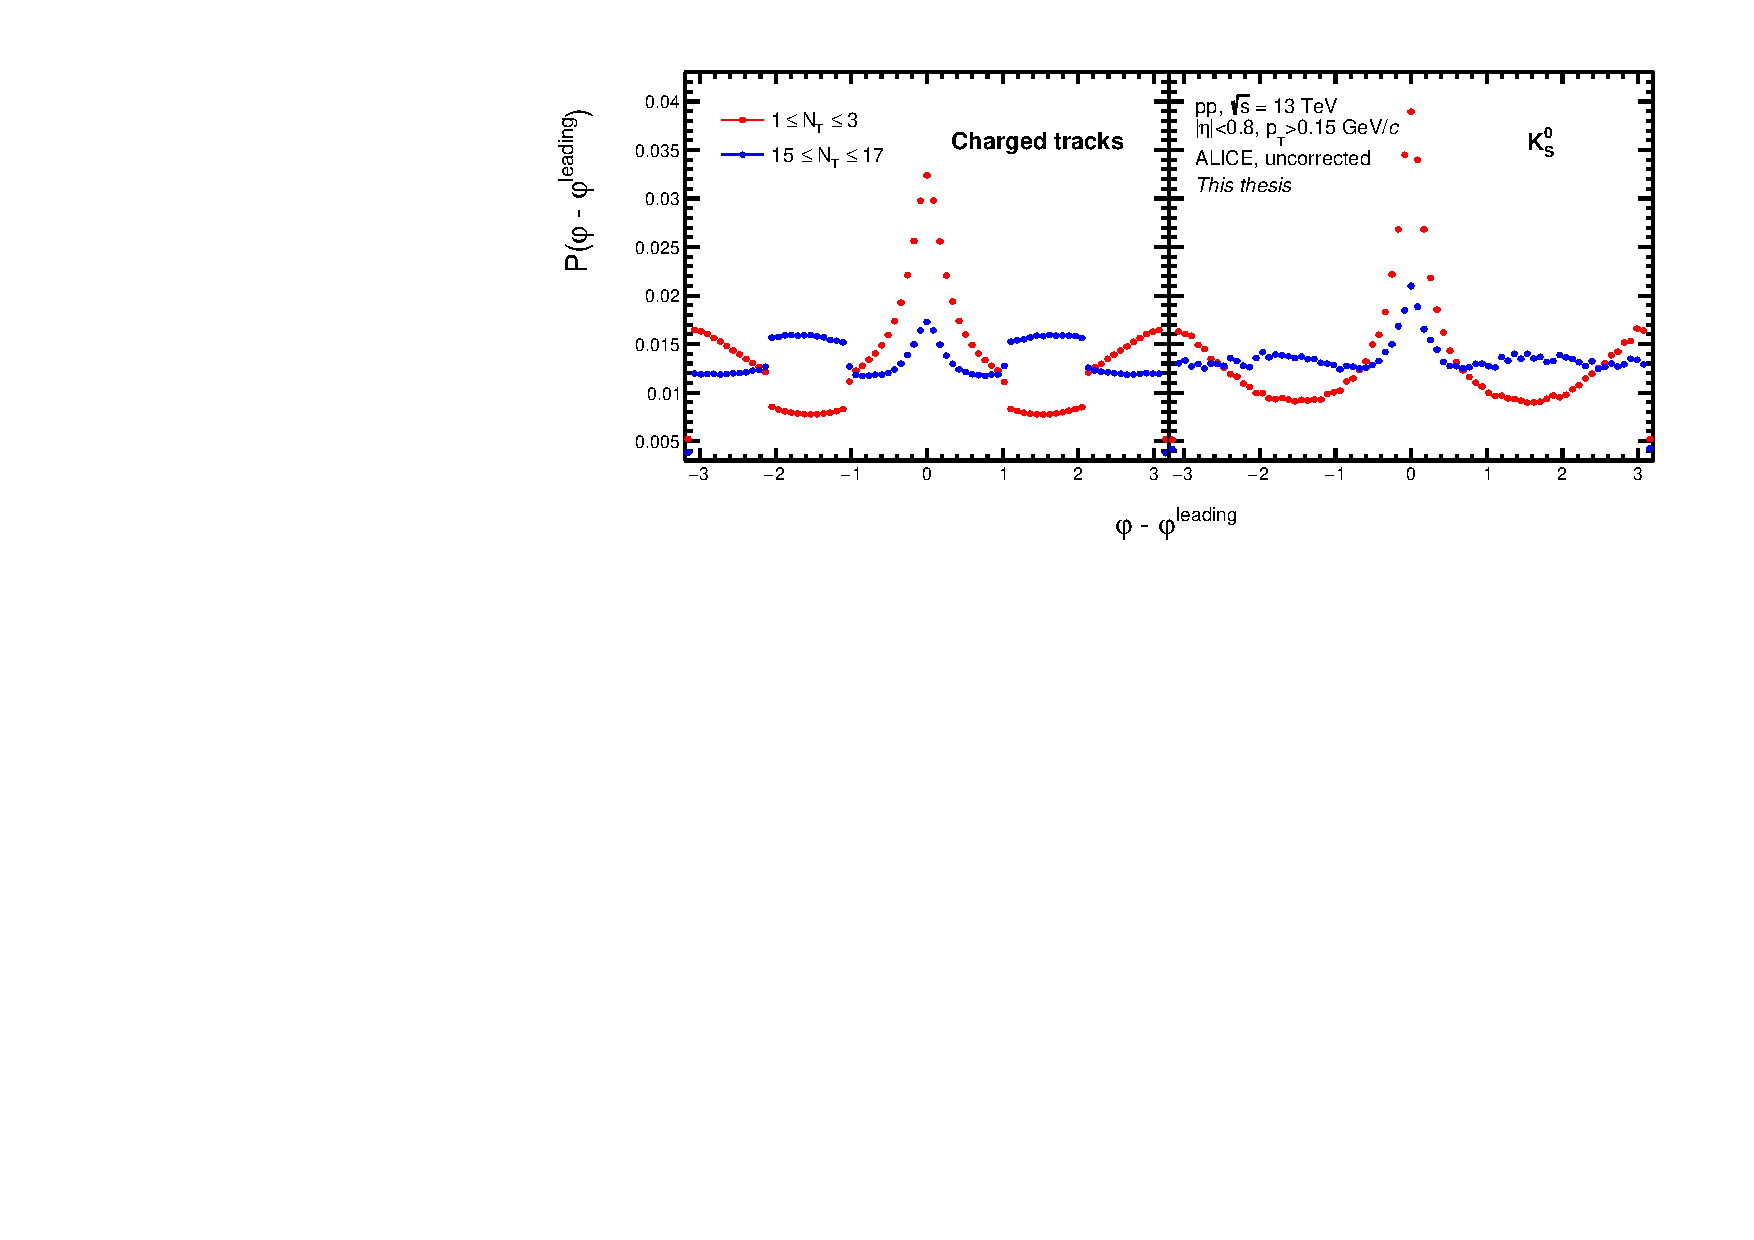
\includegraphics[width=.990\textwidth]{\imgpath/InfoRT_autocorr.pdf}}\\
\caption{TBA, maybe move to chapter about tracks.}
\label{fig:rt:autocorr}
\end{figure}


\begin{figure}%
\subfloat[][]{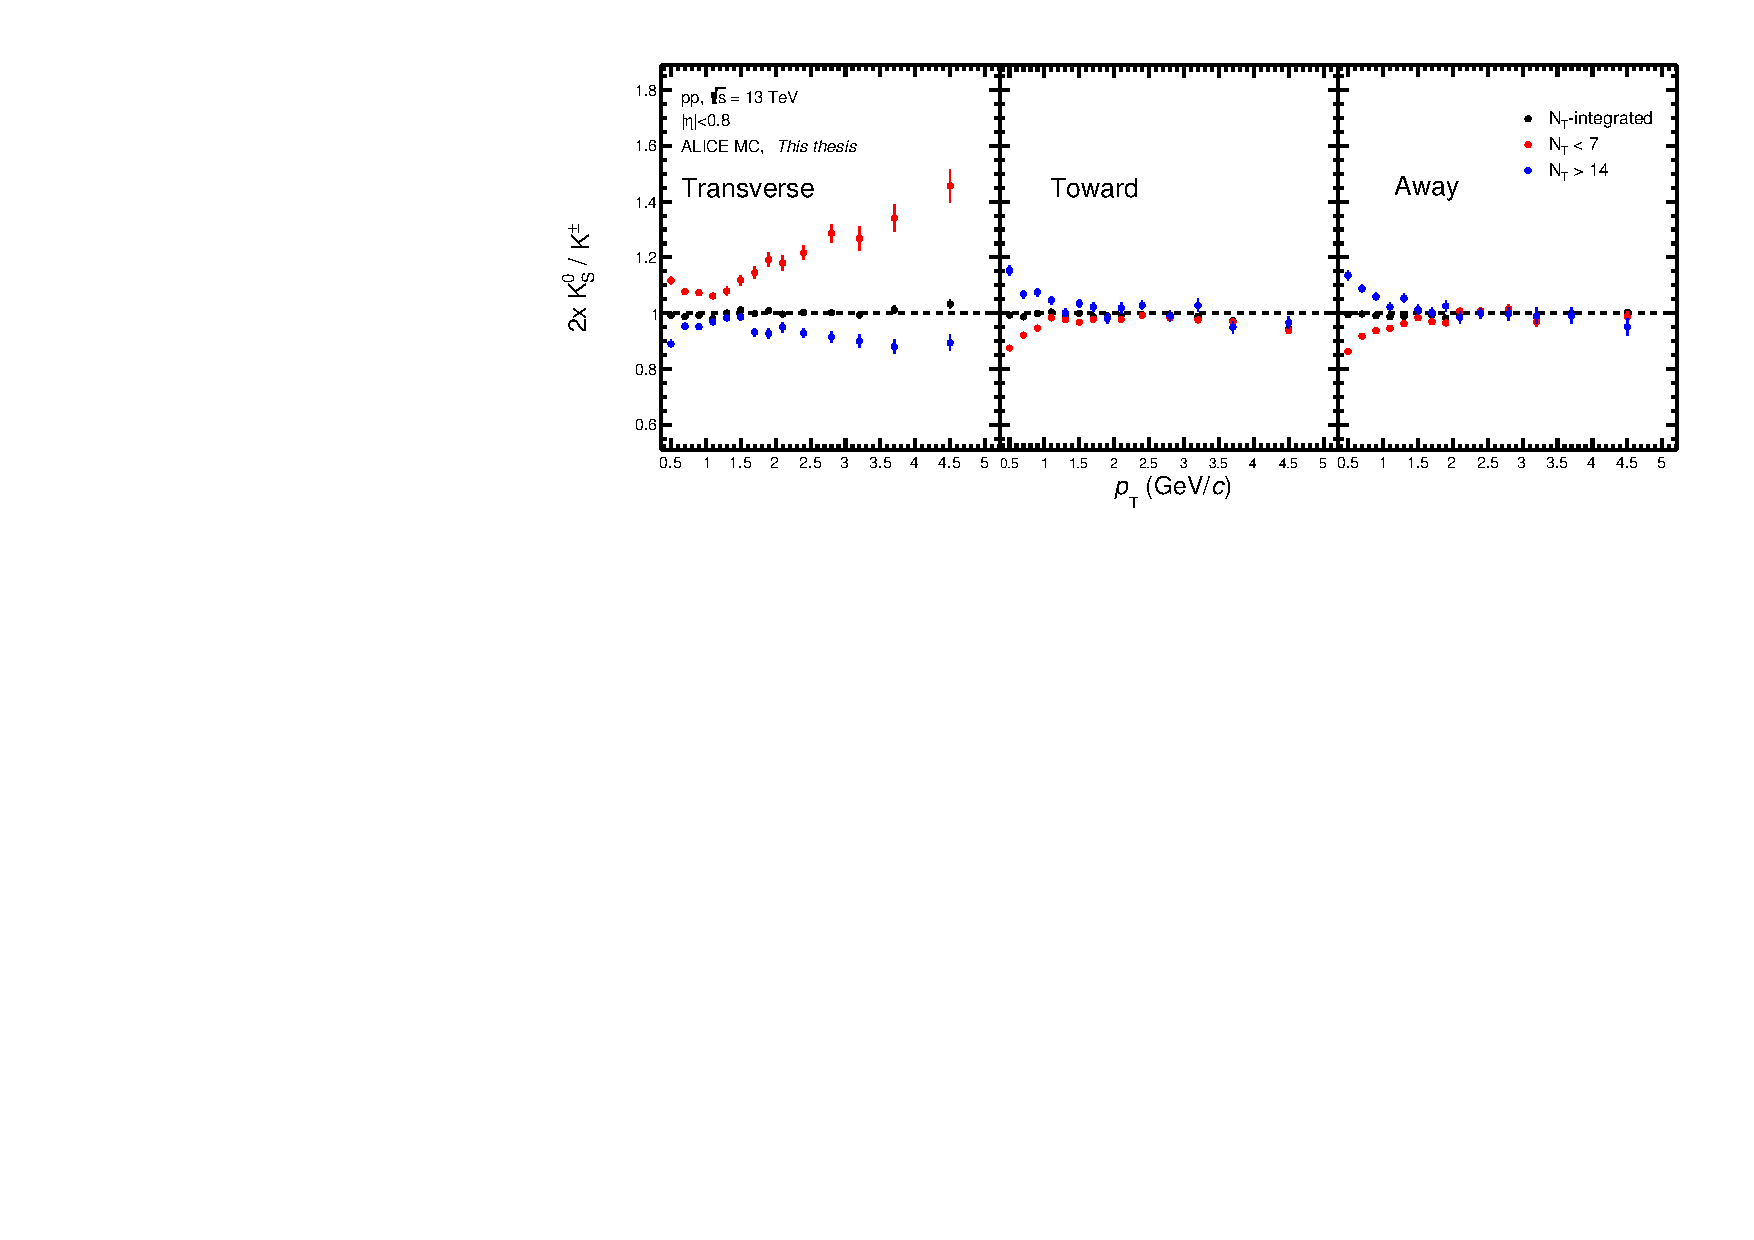
\includegraphics[width=.990\textwidth]{\imgpath/KtoK_old.pdf}}\\
\subfloat[][]{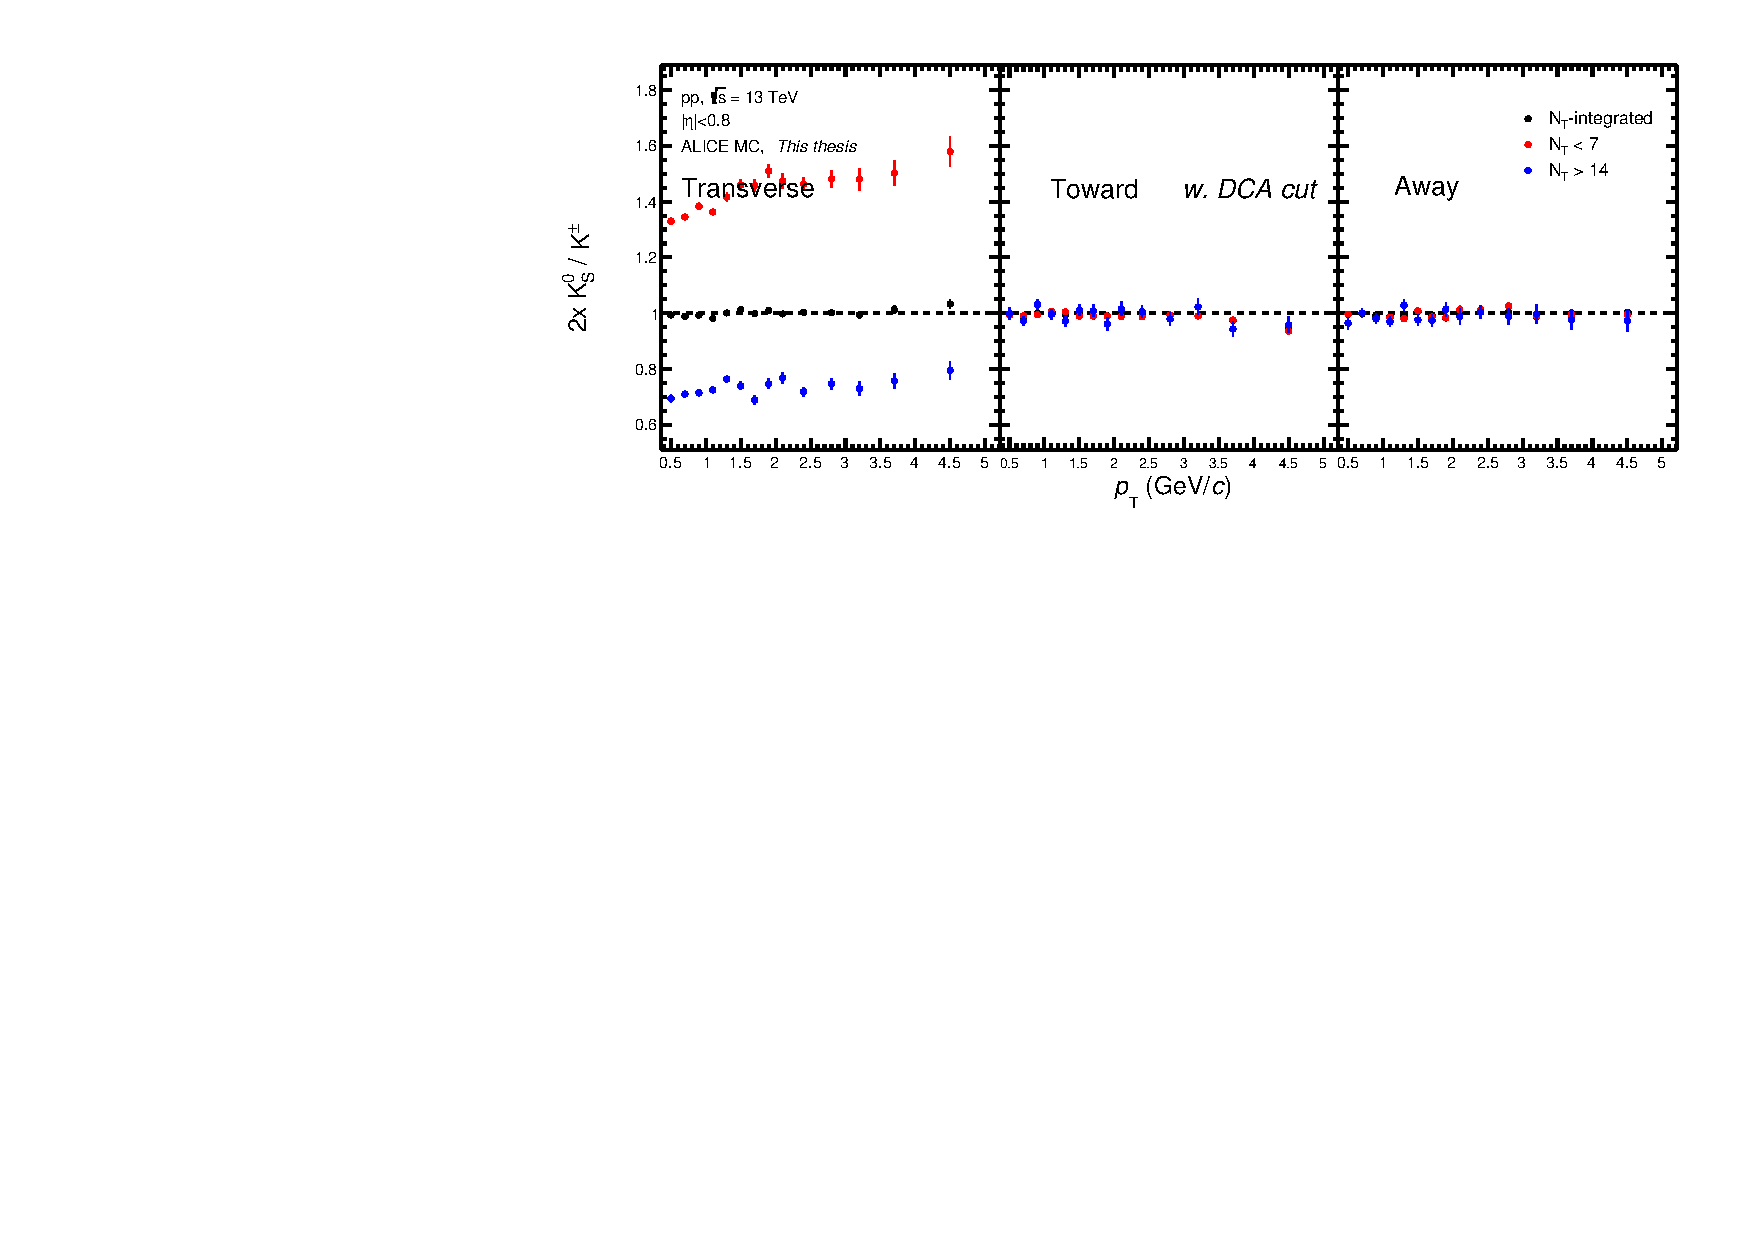
\includegraphics[width=.990\textwidth]{\imgpath/KtoK_new.pdf}}\\
\caption{TBA}
\label{fig:rt:KtoK}
\end{figure}

\begin{figure}%
\subfloat[][]{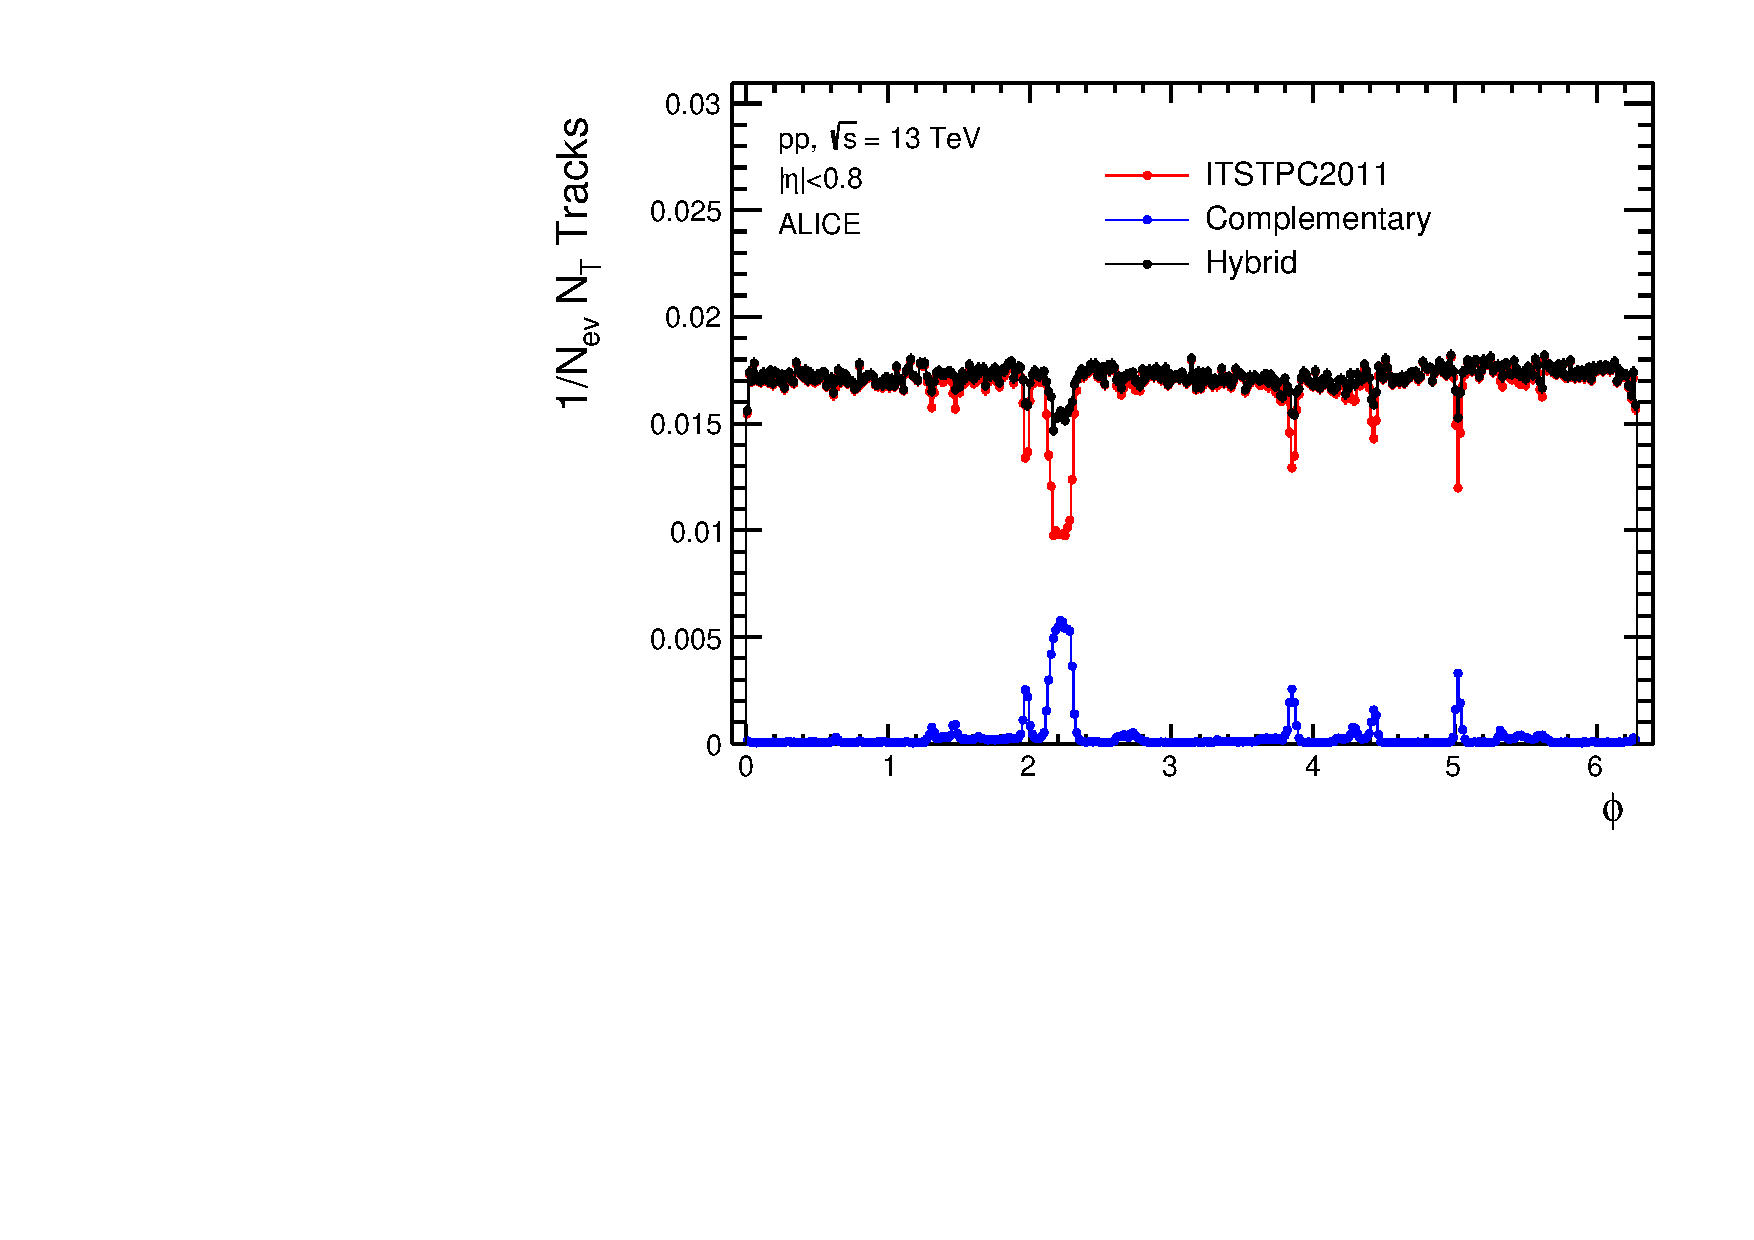
\includegraphics[width=.990\textwidth]{\imgpath/InfoRT_tracks.pdf}}\\
\caption{TBA, maybe move to chapter about tracks.}
\label{fig:rt:tracks}
\end{figure}


\section{Bayesian unfolding procedure}

The \VOs measurements are conducted as a function of the number of measured tracks \NTm within the detector acceptance. The measured multiplicity \NTm includes a fraction of the true primary charged-particle multiplicity \NTt not lost due to acceptance, efficiency, or track selection, as well as contributions from secondary particles or particles smeared into the measurement's kinematic acceptance due to detector resolution (i.e., from $\pt < \gevc{0.15}$). These effects fluctuate on an event-by-event basis and thus there is no unique correlation between \NTm and \NTt. This means that events with true multiplicity \NTt can be measured with different \NTm, contributing to \VO measurements in multiple \NTm bins. Therefore, each spectrum contains particles from events with many true multiplicities \NTt.

This thesis uses a Bayesian unfolding procedure, as discussed in Ref.~\cite{dagostini-unfolding}, to convert \VOs measurements as a function of \NTm into measurements as a function of \NTt and thus correct for the mentioned effects.

\subsection{One-dimensional unfolding}

The measured multiplicity distribution $\nev(\NTm)$ can be mathematically represented as the result of convolving (or ``folding") the true multiplicity distribution produced by the collisions, $\nev(\NTt)$, with the detector's response function. The response matrix $\mathrm{S}_{mt}$, which represents the conditional probability $P(\NTm | \NTt)$ of an event with multiplicity \NTt being measured with multiplicity \NTm, can be obtained from MC simulations of the apparatus. Using this matrix, also shown in Fig.~\ref{fig:rt:matrix}, $\nev(\NTm)$ can be expressed in terms of $\nev(\NTt)$ as follows:
\begin{align}
\nev(\NTm) = \sum_t \mathrm{S}_{mt} \cdot \nev(\NTt) \quad ,
\end{align}
To obtain the true multiplicity distribution from the measured distribution, the inverse of $S_{mt}$ could be used, hypothetically, as shown below:
\begin{align}
\nev ( \NTt ) = \sum_m \mathrm{S}_{mt}^{-1} \cdot \nev ( \NTm ) \quad .
\end{align}
However, the inverse $\mathrm{S}_{mt}^{-1}$ may have multiple or zero solutions, making this approach unfeasible. Alternatively, $\mathrm{S}_{mt}^{-1}$ could be obtained directly from MC simulations, just like the detector response. However, this matrix would then strongly depend on the generated \NTt distribution and be significantly model-dependent, as physics generators vary in their \NTt predictions. In contrast, the detector response is mostly affected by the accuracy of the particle propagation simulations, which is a lot more understood. Therefore, an iterative numerical procedure based on Bayes' theorem is used to obtain the unfolding matrix $\mathrm{M}_{mt}$, which represents the conditional probabilities $P(\NTt | \NTm)$ \cite{dagostini-unfolding}.

In this application, Bayes' theorem can be expressed in terms of \NTm and \NTt as follows,
\begin{align}
\label{eq:rt:bayes}
P(\NTt | \NTm) = \dfrac{P(\NTm | \NTt)P(\NTt)}{P(\NTm)} \quad ,
\end{align}
where $P(\NTt)$ and $P(\NTm)$ are probability distributions for an event occurrence with \NTt and \NTm, respectively. Assuming that $P(\NTt)$ is known, $P(\NTm)$ can be calculated as follows:
\begin{align}
P(\NTm) = \sum_t P(\NTm | \NTt) P(\NTt) \quad .
\end{align}
Therefore, using Eq.~\ref{eq:rt:bayes}, the conditional probability in the unfolding matrix can be written as follows:
\begin{align}
P(\NTt | \NTm) = \dfrac{P(\NTm | \NTt)P(\NTt)}{\sum_{t'} P(\NTm | \NTtt) P(\NTtt)} \quad .
\end{align}

However, $P(\NTt)$ (the ``prior") is initially unknown and must be arbitrarily chosen. The unfolding matrix can be calculated using this prior, and the unfolded distribution can be obtained as follows:
\begin{align}
\nevhat(\NTt) = \sum_m P(\NTt | \NTm) \nev(\NTm) \quad .
\end{align}
This unfolded multiplicity can subsequently be used to update the prior as follows:
\begin{align}
\hat{P}(\NTt) = \dfrac{\nevhat(\NTt)}{\sum_{t'} \nevhat(\NTtt)} \quad ,
\end{align}
starting a new iteration. The updated $\hat{P}(\NTt)$ is closer to the true $P(\NTt)$ than the initial guess because the arbitrarily chosen prior is constrained by the $\nev(\NTm)$ observable, which contains information about $P(\NTt)$.

Multiple approaches can be taken to choose the prior: a uniform distribution, the $\NTt$ distribution generated by a model, or the $\NTm$ distribution acquired from data. In this thesis, the prior choice was found to not play a role.

TBA: Normalisation

The $\chi^2/\mathrm{ndf}$ is calculated to determine the validity of the correction and the stopping point for the iterative process. It is calculated by comparing the $\NTt$ distribution -- known a priori in the simulations -- and the unfolded $\nevhat(\NTt)$ distribution, where $\mathrm{ndf}$ refers to the number of data points in the distribution. The process is stopped when $\chi^2/\mathrm{ndf}$ reaches a minimum value or the iterations take a maximum number of steps $n_\mathrm{iter}$. This is imposed to avoid overfitting and overestimation of statistical uncertainties. The $n_\mathrm{iter}$ values are reported in Tab.~\ref{tab:rt:niter}. The entire iterative process is summarised in a diagram shown in Fig.~\ref{fig:rt:bayes}. 

The used response matrix, as well as the resulting unfolding matrix, can be seen in Fig.~\ref{fig:rt:matrix}. The method still exhibits some degree of model dependence due to the generation of the response matrix. Previous studies in ALICE have compared the response matrix for \NT acquired from Pythia 8 and from EPOS LHC MC simulations, which revealed that the effect is less than $1\%$. This effect is taken into consideration as a source of systematic uncertainty.

\begin{table}[h!]
\centering
\caption{TBA.}
\label{tab:rt:niter}

\begin{tabular}{|cc|ccc|}
\hline
\multicolumn{2}{|r|}{\parbox[b][1.2em]{2em}{} Unfolding observable} & \NT & \NTmin & \NTmax I \\ \hline
\multicolumn{2}{|l|}{\parbox[b][1.1em]{1em}{}$n_\mathrm{iter}$} & $20$ (max.) & $10$ & $18$ \\ \hline
\end{tabular}
\end{table}


\begin{figure}[h]
		\centering
		\begin{tikzpicture}[node distance=0.8cm,box/.style={draw, rounded corners=.2cm}]
			%\node[box, text width=0.9\textwidth, align=center] (eqn) {\NTt ...\ true multiplicity};
			%below=of eqn
			\node[box, fill=black!10, text width=0.9\textwidth, align=center] (thm) {Bayes' Theorem\\\vspace{1em}$P(\NTt | \NTm) = \dfrac{P(\NTm | \NTt)P(\NTt)}{P(\NTm)}$};
			\node[box, below=of thm, align=center] (f1) {Unfolding matrix\\
			\\$P(\NTt | \NTm) = \dfrac{P(\NTm | \NTt)P(\NTt)}{\sum_{t'}P(\NTm | \NTtt)P(\NTtt)}$};
			\node[draw=none, below=of f1, align=center] (f2) {\begin{Large}$\times \, n_\mathrm{iter}$\end{Large}};
			\node[draw=none, below=of f2, align=center] (f0) {};
			\node[box, left=of f0, text width=.47\textwidth,text height=1em, align=center] (f3) {Unfolded distribution\\\vspace{1em}$\nevhat(\NTt) = \sum_m P(\NTt | \NTm) \nev(\NTm)$};
			\node[box, right=of f0, text width=.40\textwidth, text height=1em, align=center] (f4) {Updated prior\\\vspace{0.5em}$\hat{P}(\NTt) = \dfrac{\nevhat(\NTt)}{\sum_{t'} \nevhat(\NTtt)}$};
			\draw[-{Latex[bend]}, ultra thick, blue] (f1) to[bend right=50] (f3);
			\draw[-{Latex[bend]},ultra thick, blue] (f3) to[bend right] (f4);
			\draw[-{Latex[bend]},ultra thick, blue] (f4) to[bend right=50] (f1);
		\end{tikzpicture}
		\caption{Diagram showing the Bayesian unfolding}
		\label{fig:rt:bayes}
\end{figure}

\begin{figure}%
\subfloat[][]{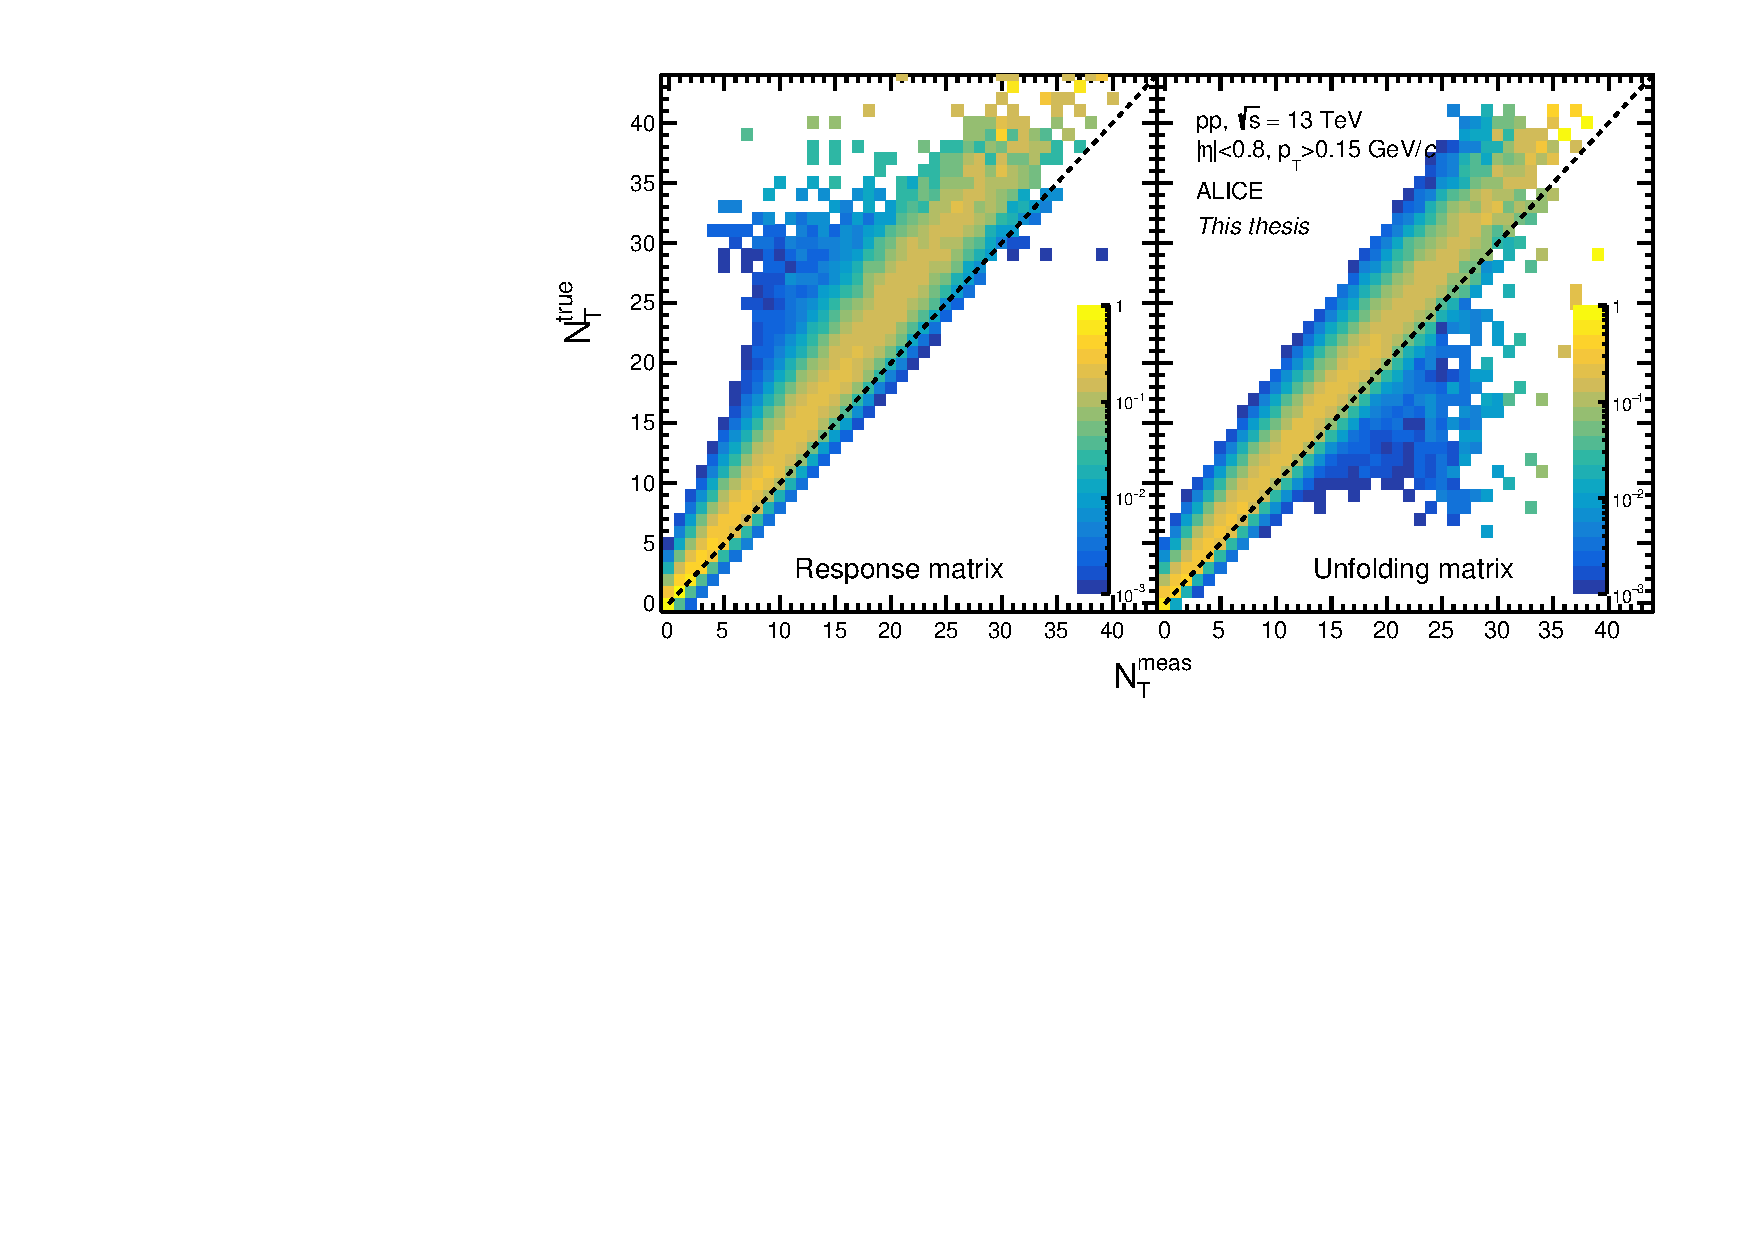
\includegraphics[width=.990\textwidth]{\imgpath/InfoRT_matrix.pdf}}\\
\caption{TBA}
\label{fig:rt:matrix}
\end{figure}

\subsection{Propagation of statistical uncertainties}

TBA

\subsection{Unfolding of \KOs, \LA, and \AL \pt spectra}

TBA

\section{\RT, \RTmin, \RTmax distributions}

The unfolded \NT, \NTmin, and \NTmax distributions were self-normalised to obtain the \RT, \RTmin, and \RTmax distributions, respectively. They are shown in Fig.~\ref{fig:rt:rtdistr} and compared with predictions from Pythia 8 (Monash tune and Ropes tune) as well as EPOS LHC. The different quantiles corresponding to the $\RT/\RTmin/\RTmax$ ranges used in this measurement are also highlighted. It should be noted that since $\NT, \NTmin, \NTmax \in \mathbb{N}_0$, the $\RT/\RTmin/\RTmax$ distributions are not continuous observables.

\begin{figure}%
\subfloat[][]{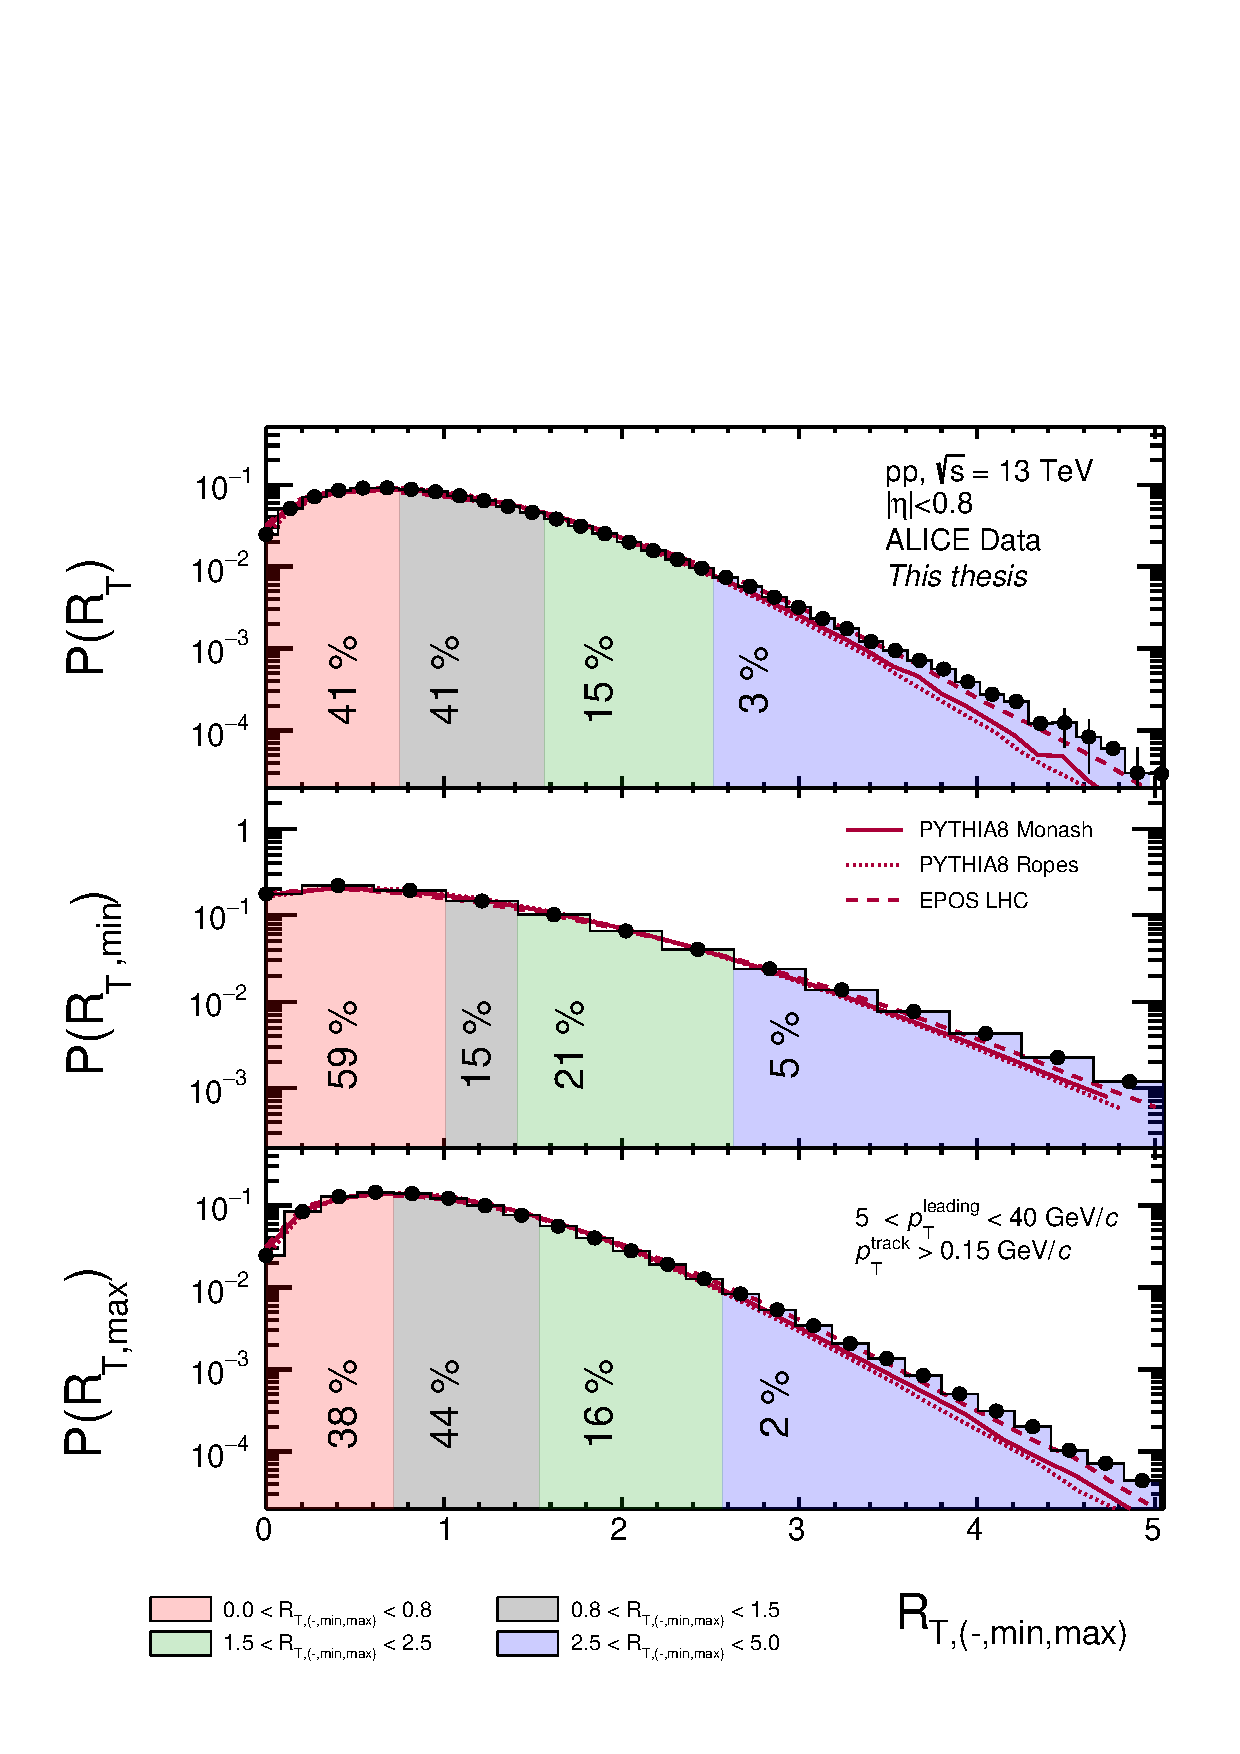
\includegraphics[width=.990\textwidth]{\imgpath/Rt_distr.pdf}}\\
\caption{TBA}
\label{fig:rt:rtdistr}
\end{figure}

\section{Systematic uncertainties}

The systematic uncertainties on the \pt spectra were determined individually for each \RT interval and azimuthal region, following the procedures described in Section~\ref{sec:ana:syst}. They are reported in Fig.~\ref{fig:rt:systK0s}, Fig.~\ref{fig:rt:systLA}, and Fig.~\ref{fig:rt:systAL} for the \KOs, \LA, and \AL, respectively. As there are no reasons to believe they should differ, they are then also applied in the \RTmin and \RTmax measurements.

TBA comment on the largest ones

\begin{figure}%
\subfloat[][]{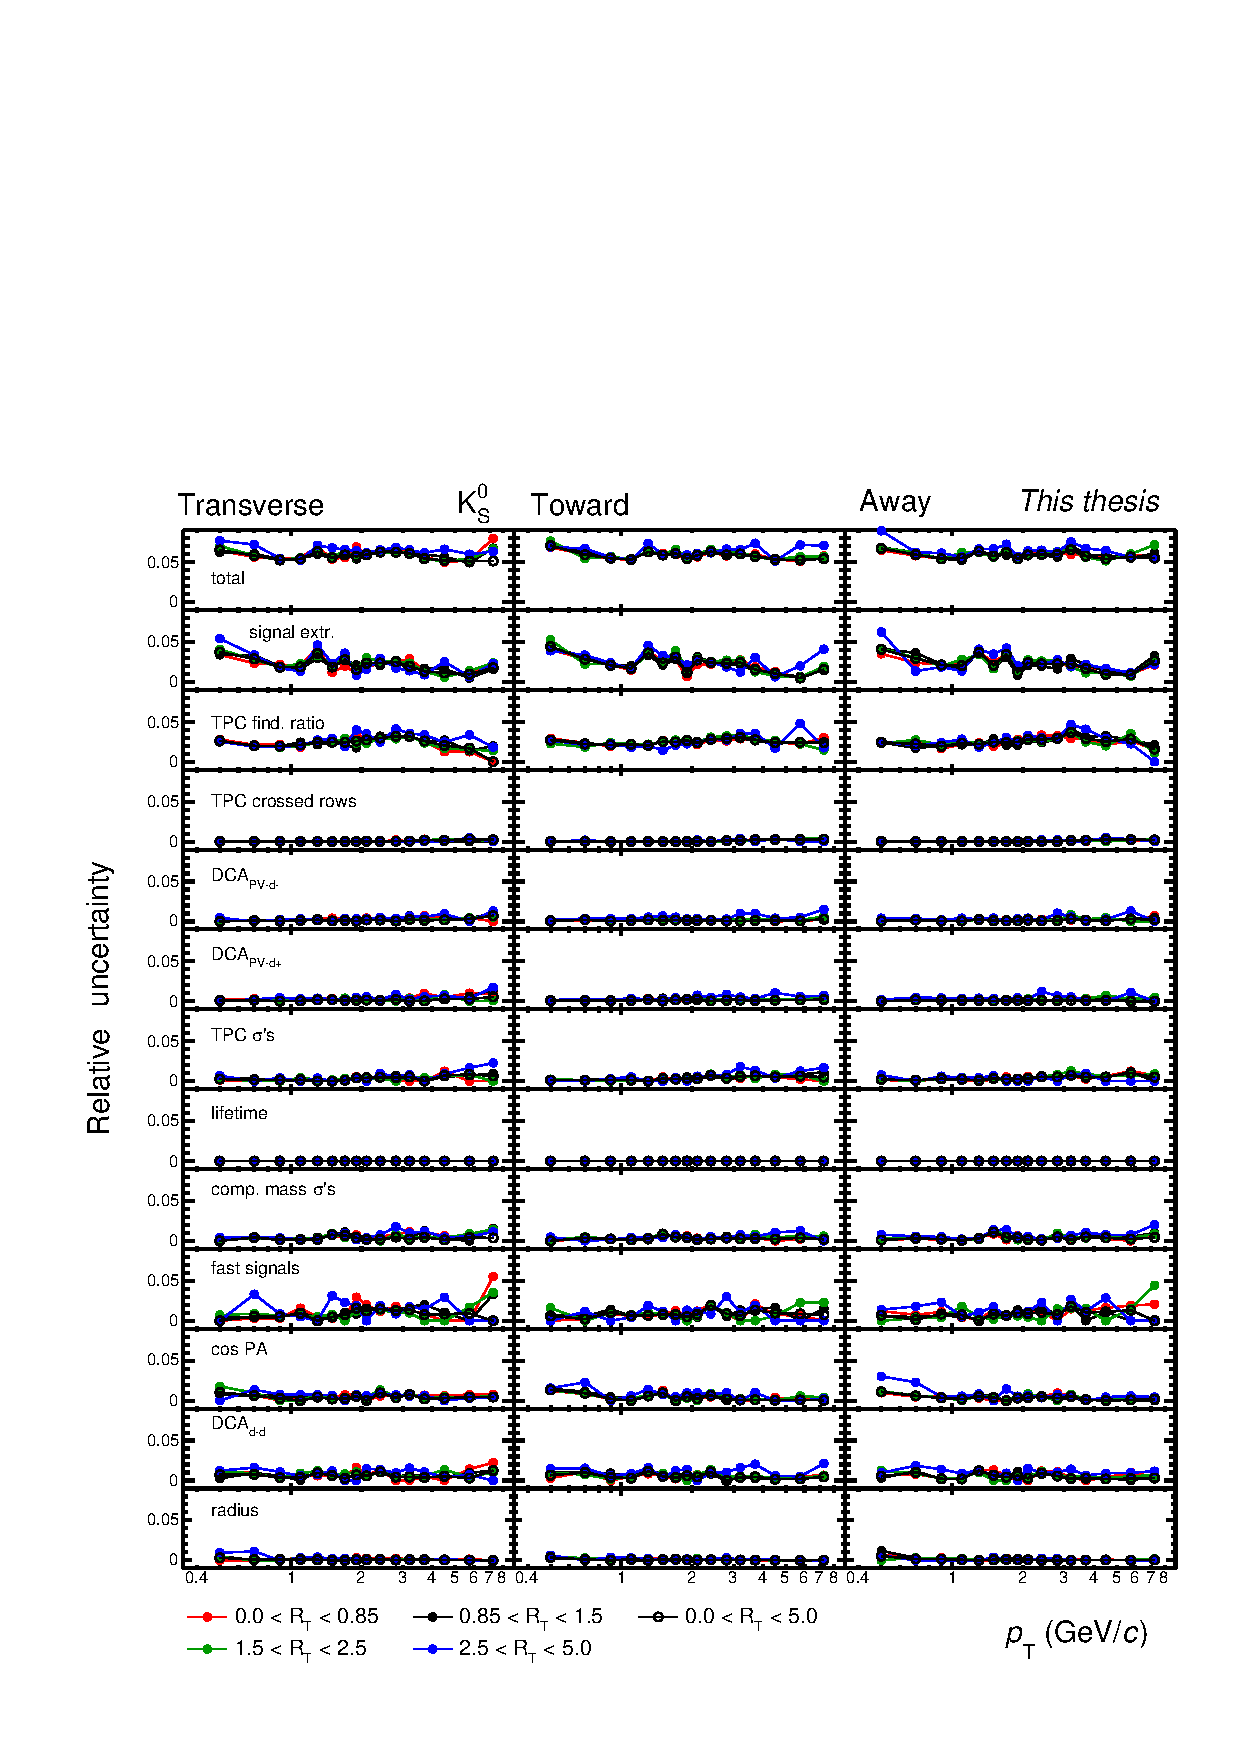
\includegraphics[width=.990\textwidth]{\imgpath/InfoRT_syst_K0s.pdf}}\\
\caption{TBA.}
\label{fig:rt:systK0s}
\end{figure}

\begin{figure}%
\subfloat[][]{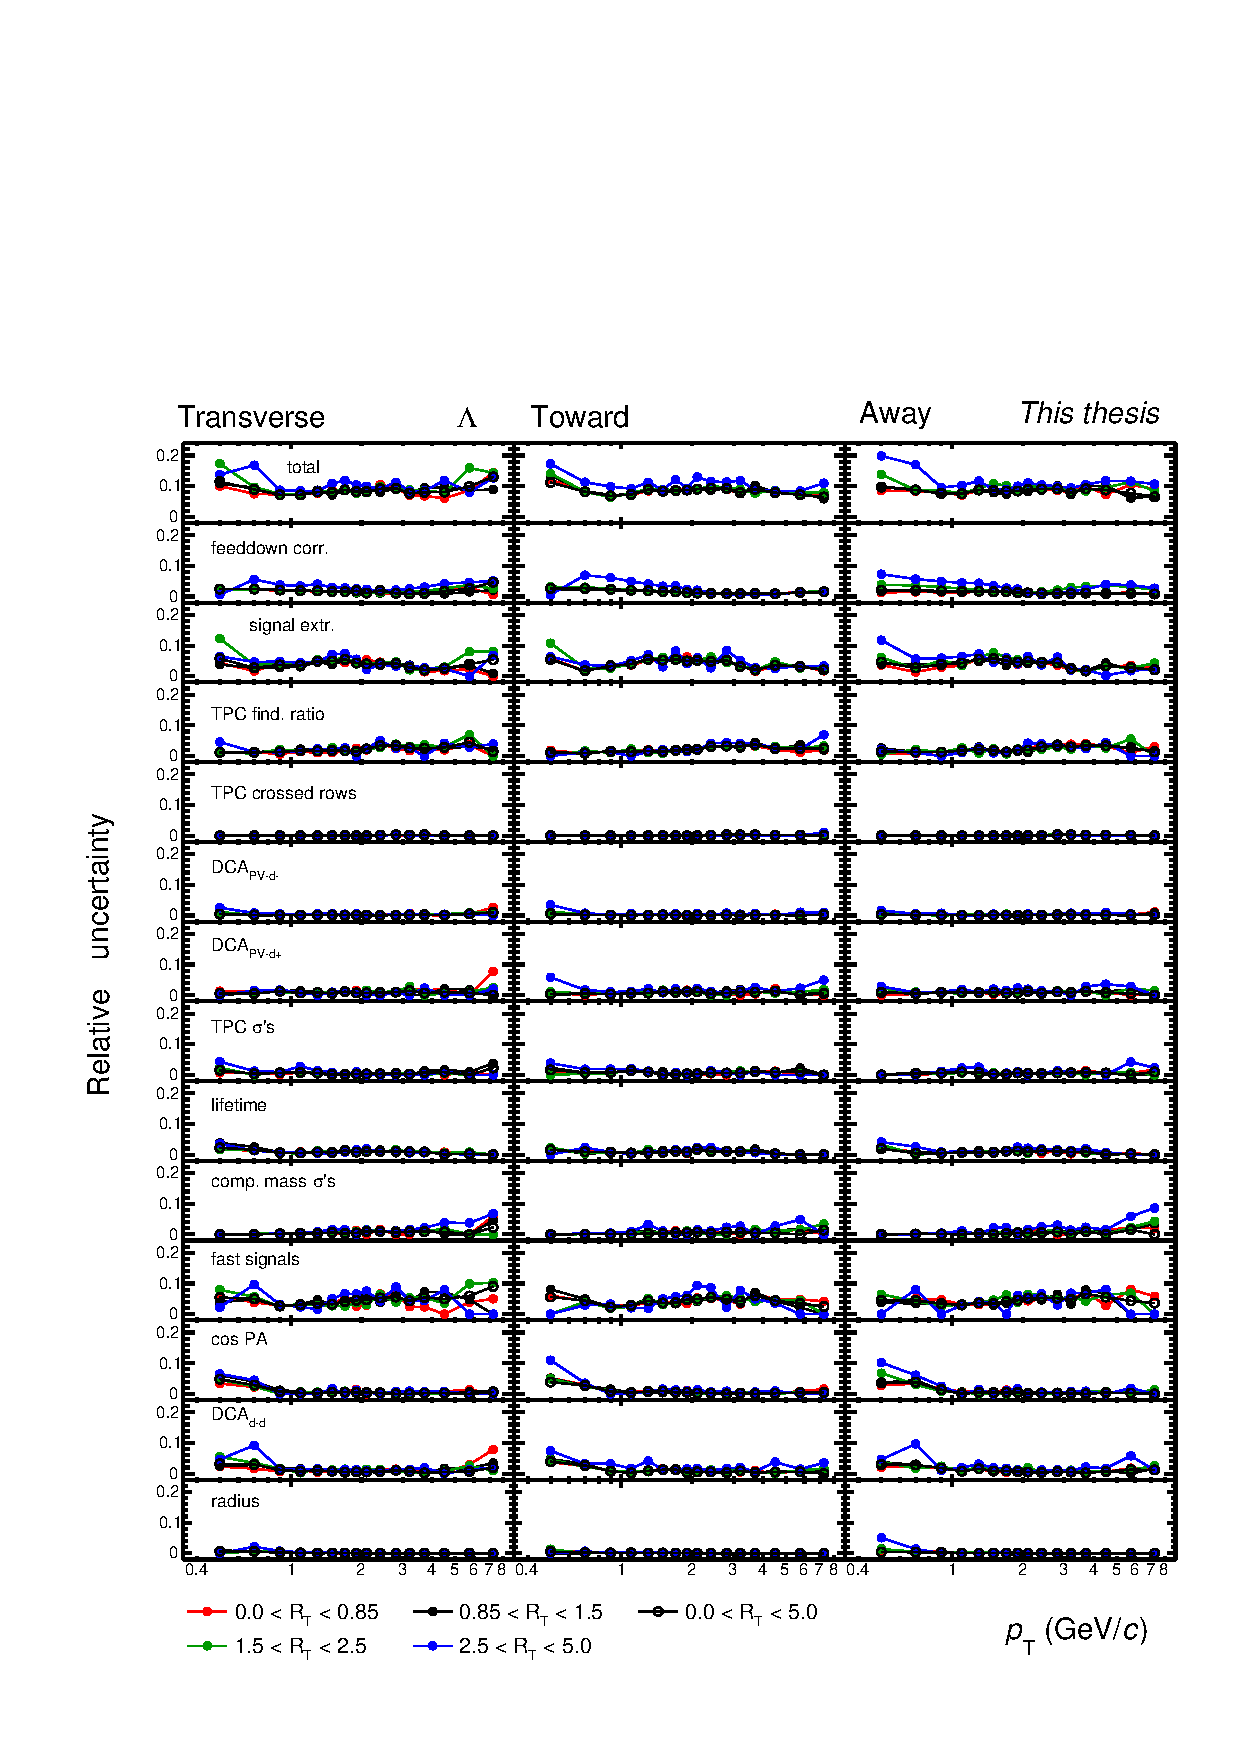
\includegraphics[width=.990\textwidth]{\imgpath/InfoRT_syst_L.pdf}}\\
\caption{TBA.}
\label{fig:rt:systL}
\end{figure}

\begin{figure}%
\subfloat[][]{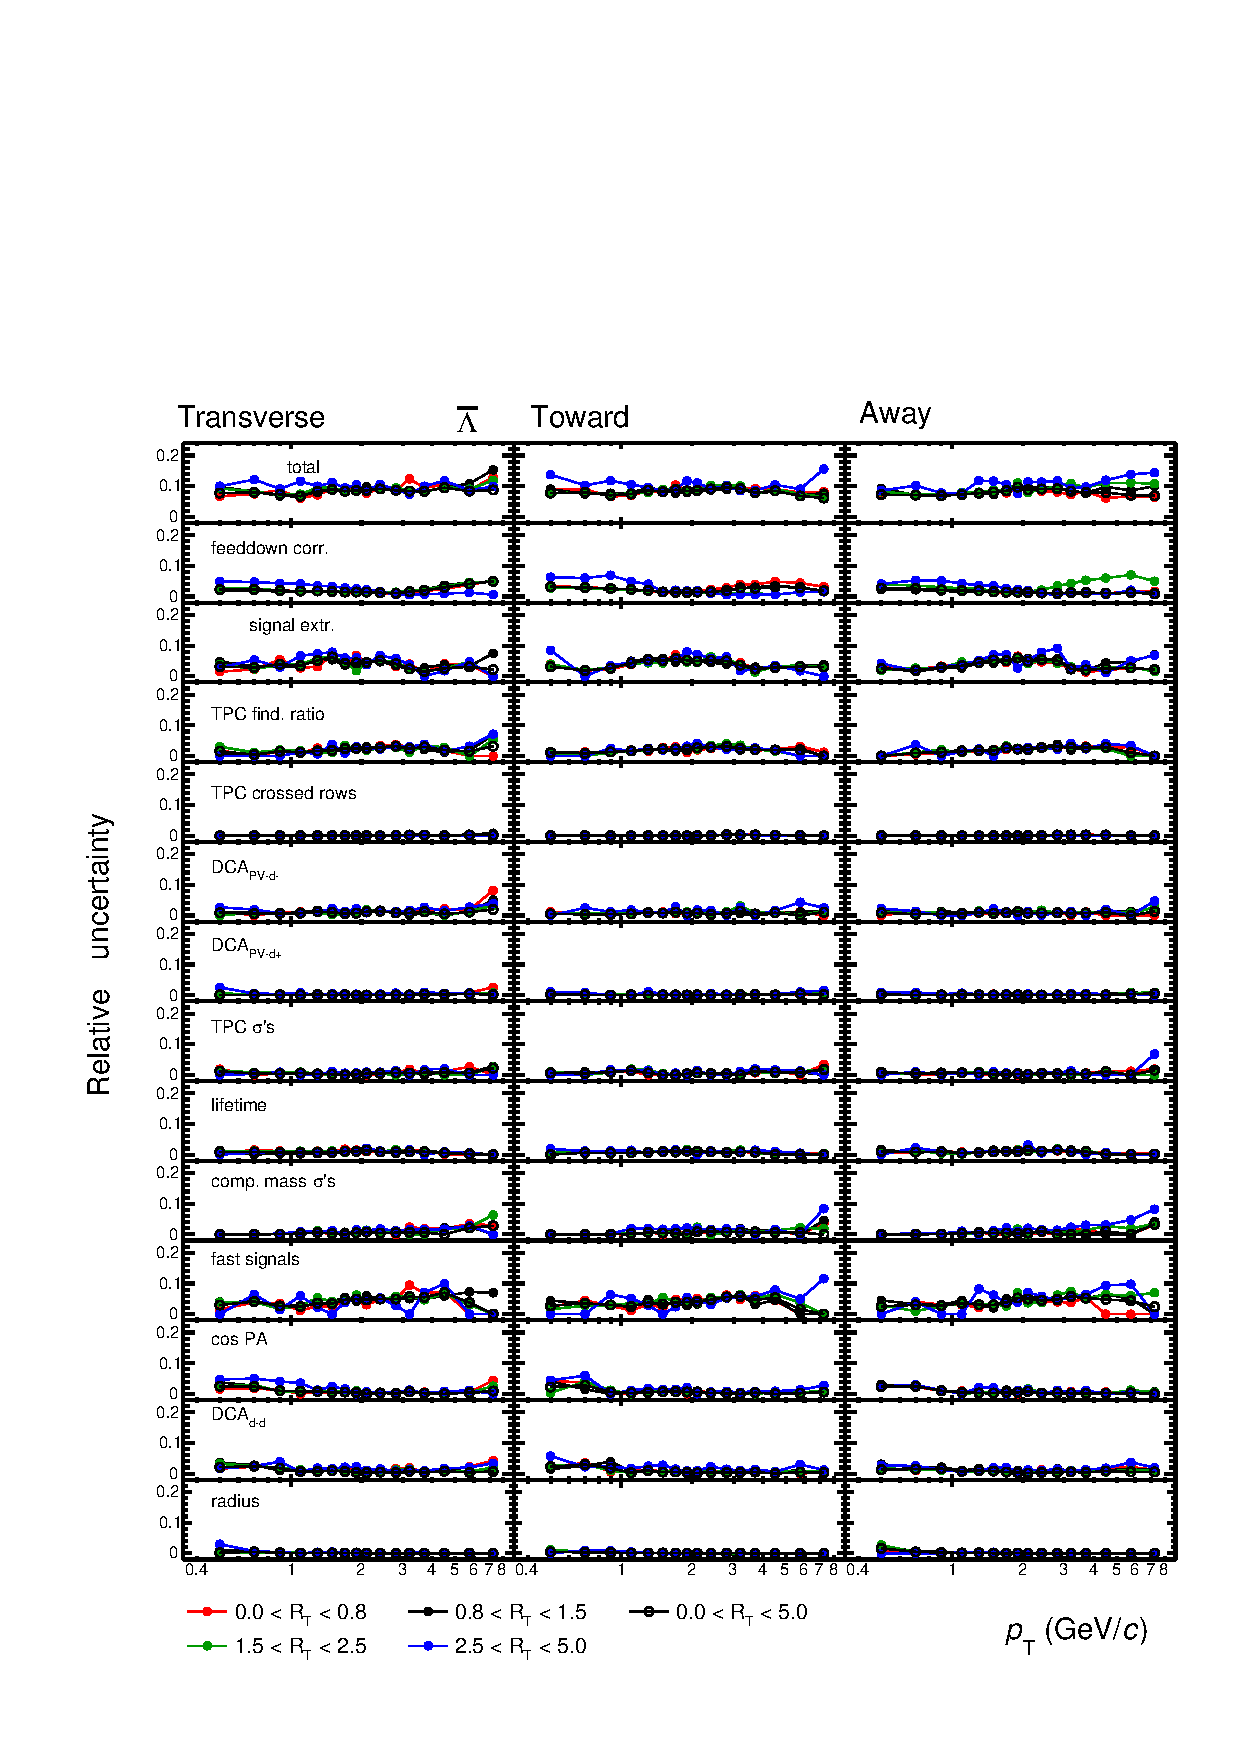
\includegraphics[width=.990\textwidth]{\imgpath/InfoRT_syst_Lbar.pdf}}\\
\caption{TBA.}
\label{fig:rt:systLbar}
\end{figure}

\subsection{Uncertainties from the unfolding procedure}

TBE

The deviations between the generated \pt spectra and the reconstructed, corrected, and unfolded \pt spectra were used to determine the systematic uncertainties associated with the unfolding procedure. To isolate the effect of unfolding from other reconstruction effects, the ``non-closures" in each $\RT/\RTmin/\RTmax$ interval were divided by the non-closure in the $\RT/\RTmin/\RTmax$-integrated bin.

The unfolding systematic uncertainties exhibited a large amount of correlation between \KOs and \LA. This correlation was expected, as the \VO species shouldunfold in similar patterns. Therefore, the systematic uncertainty on the baryon-to-meson ratio was also calculated independently to avoid these correlations and reduce the systematic uncertainty on those results.

Moreover, in the most extreme bins, the non-closures sometimes exhibited unrealistic deviations from unity due to limited statistics and fluctuations. To address this issue, a smoothing procedure was applied by fitting the resulting uncertainties with first- and second-order polynomials. The results are shown in Fig.~\ref{fig:rt:systUnf}.

\begin{figure}%
\subfloat[][]{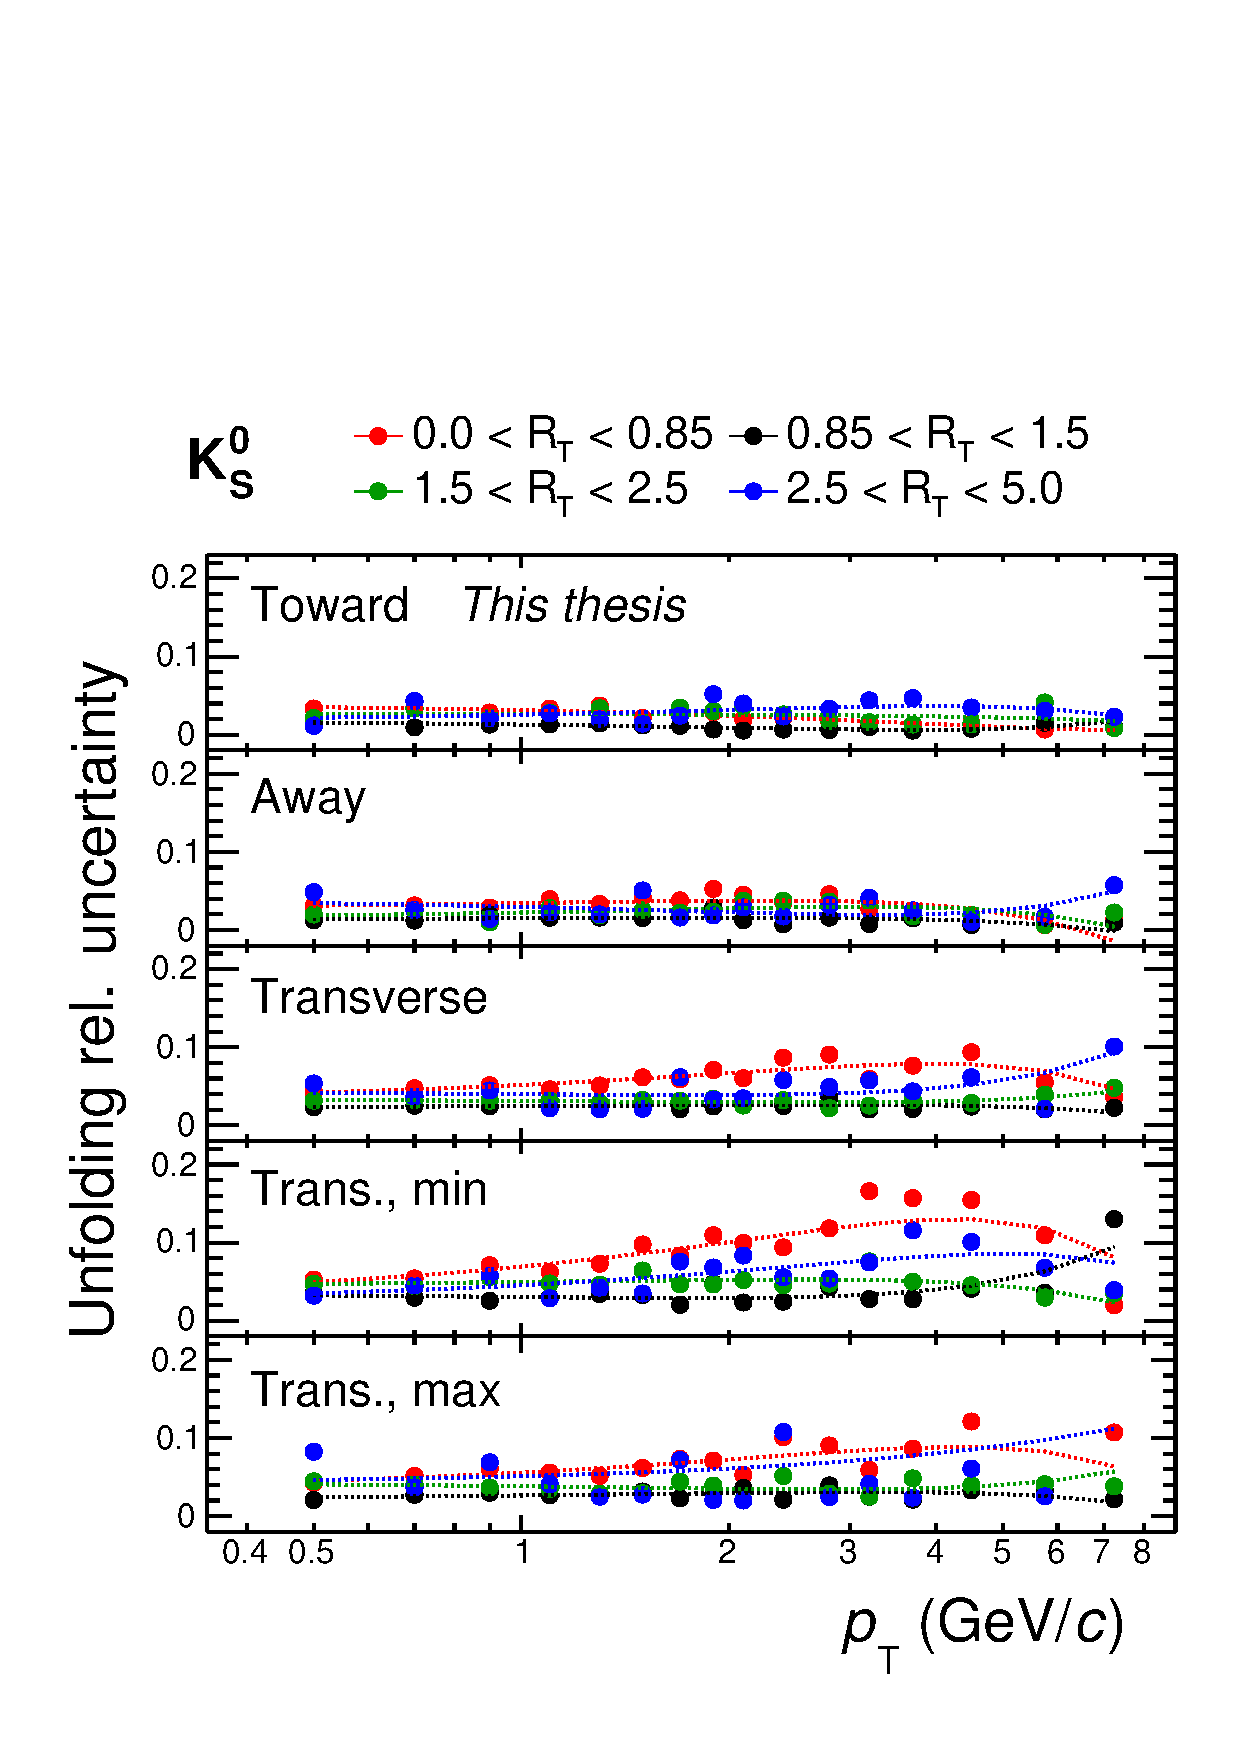
\includegraphics[width=.320\textwidth]{\imgpath/InfoRT_systUnf_K0s.pdf}}
\subfloat[][]{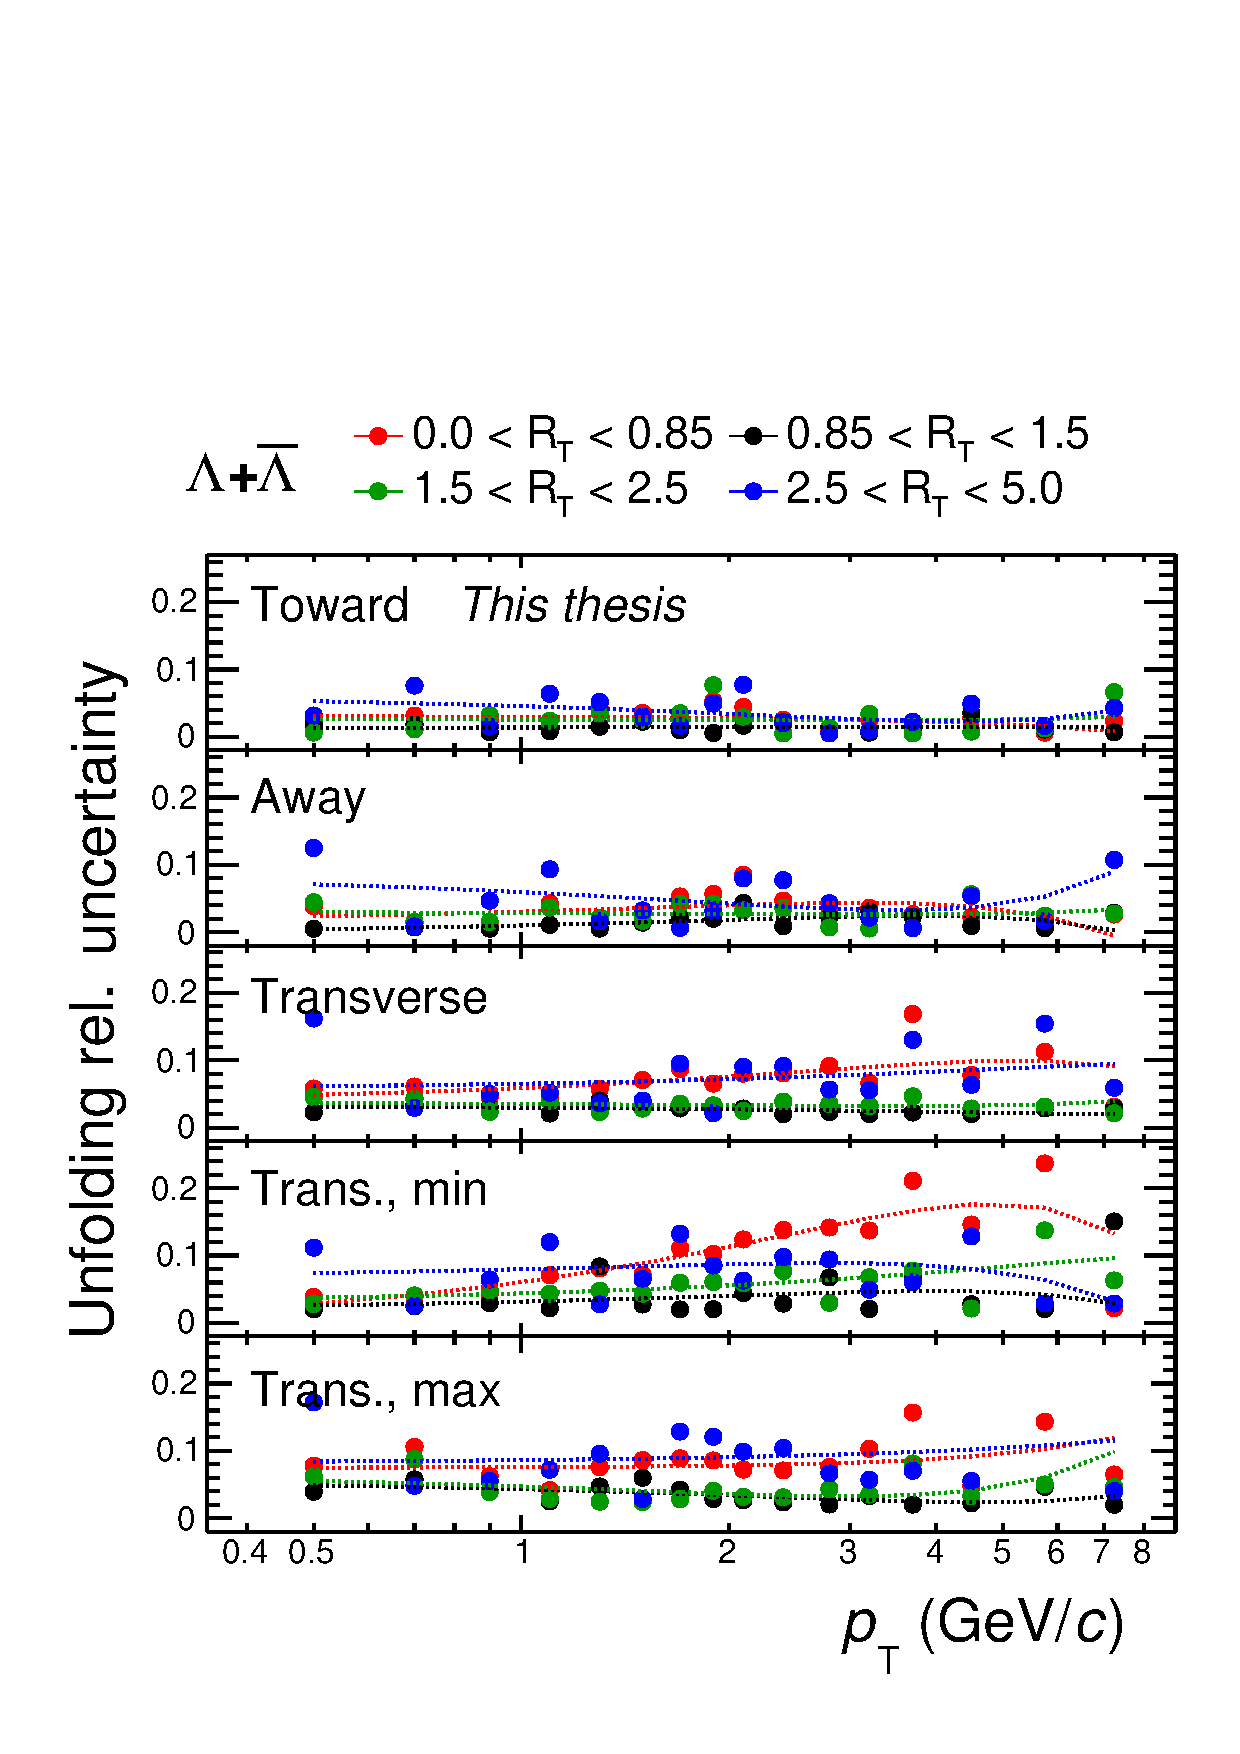
\includegraphics[width=.320\textwidth]{\imgpath/InfoRT_systUnf_L.pdf}}
\subfloat[][]{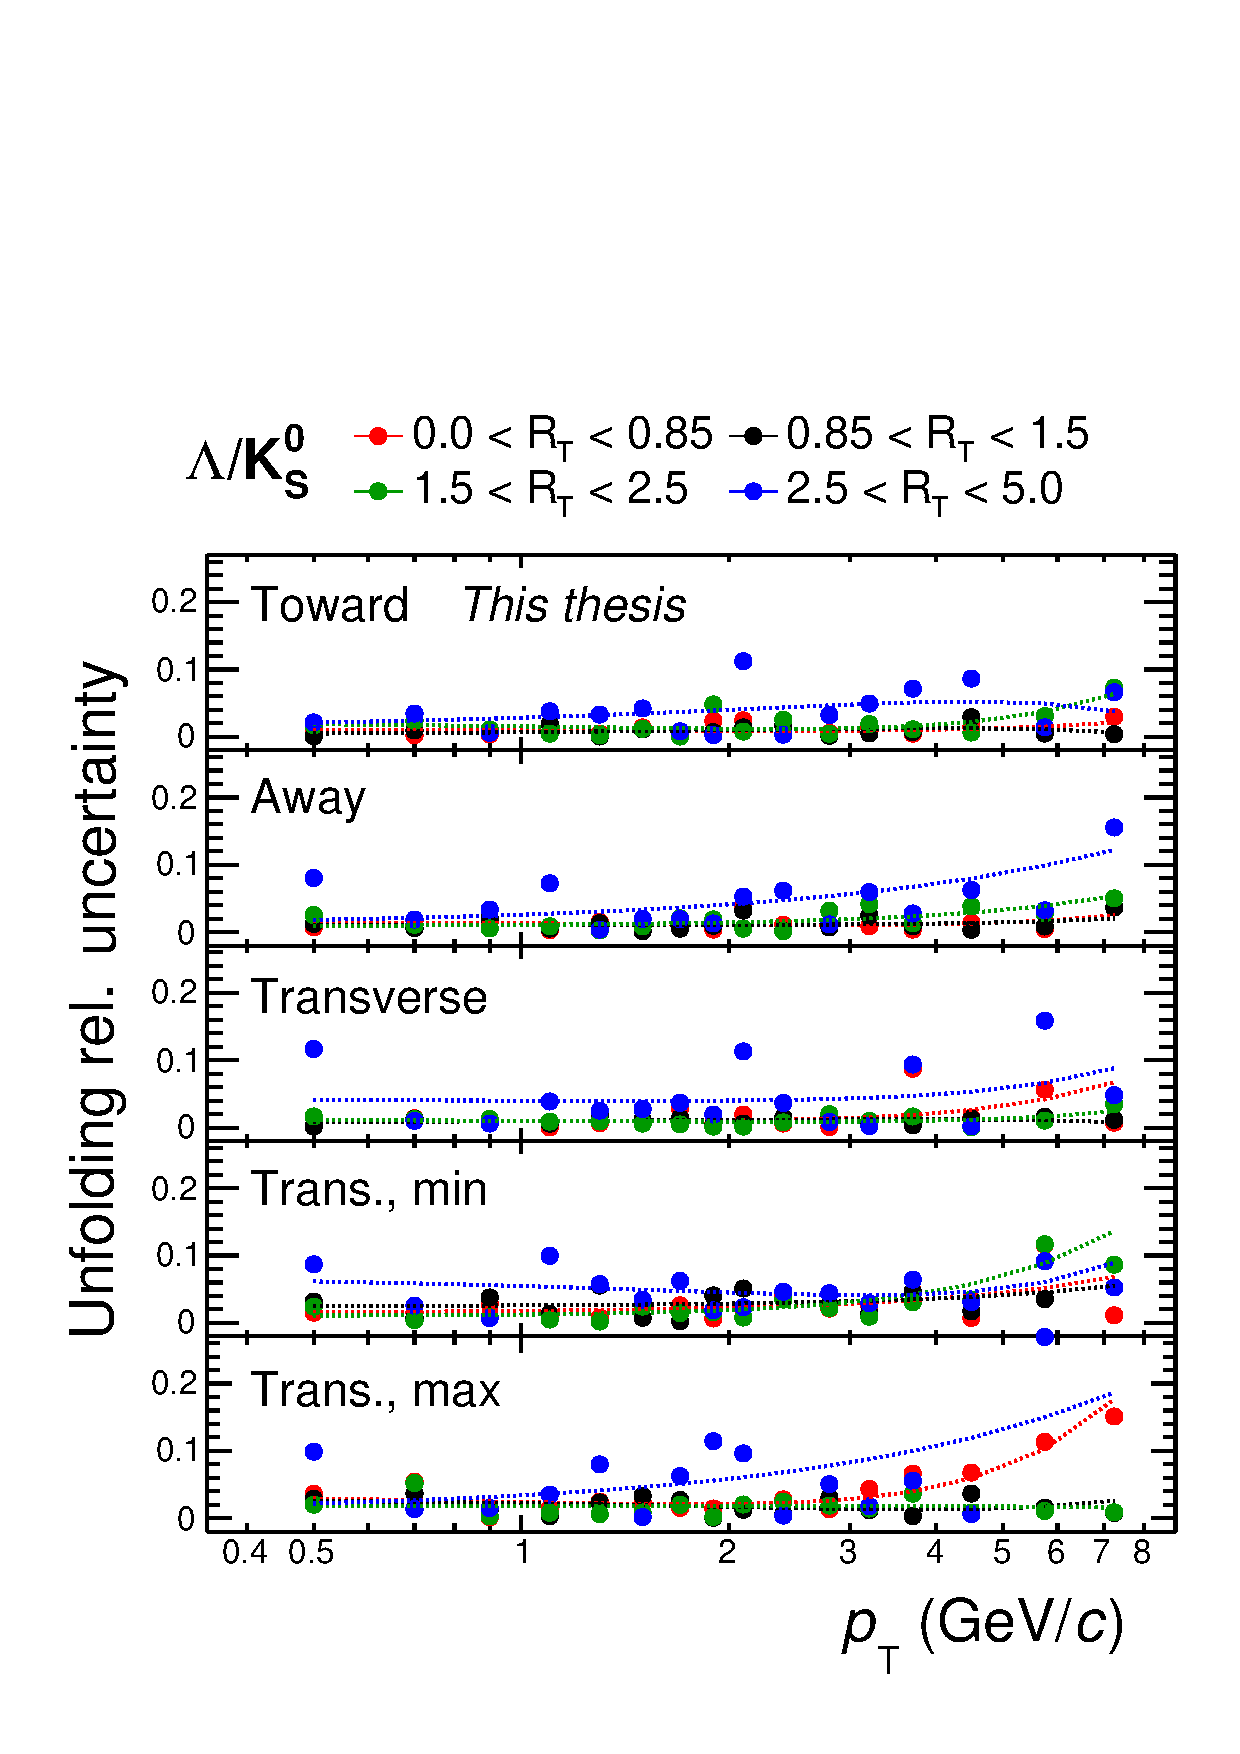
\includegraphics[width=.320\textwidth]{\imgpath/InfoRT_systUnf_LtoK0s.pdf}}
\caption{TBA.}
\label{fig:rt:systUnf}
\end{figure}

\subsection{Uncorrelated uncertainties}

TBA

\section{Mean transverse momentum}

TBA
 
\begin{figure}%
\subfloat[][]{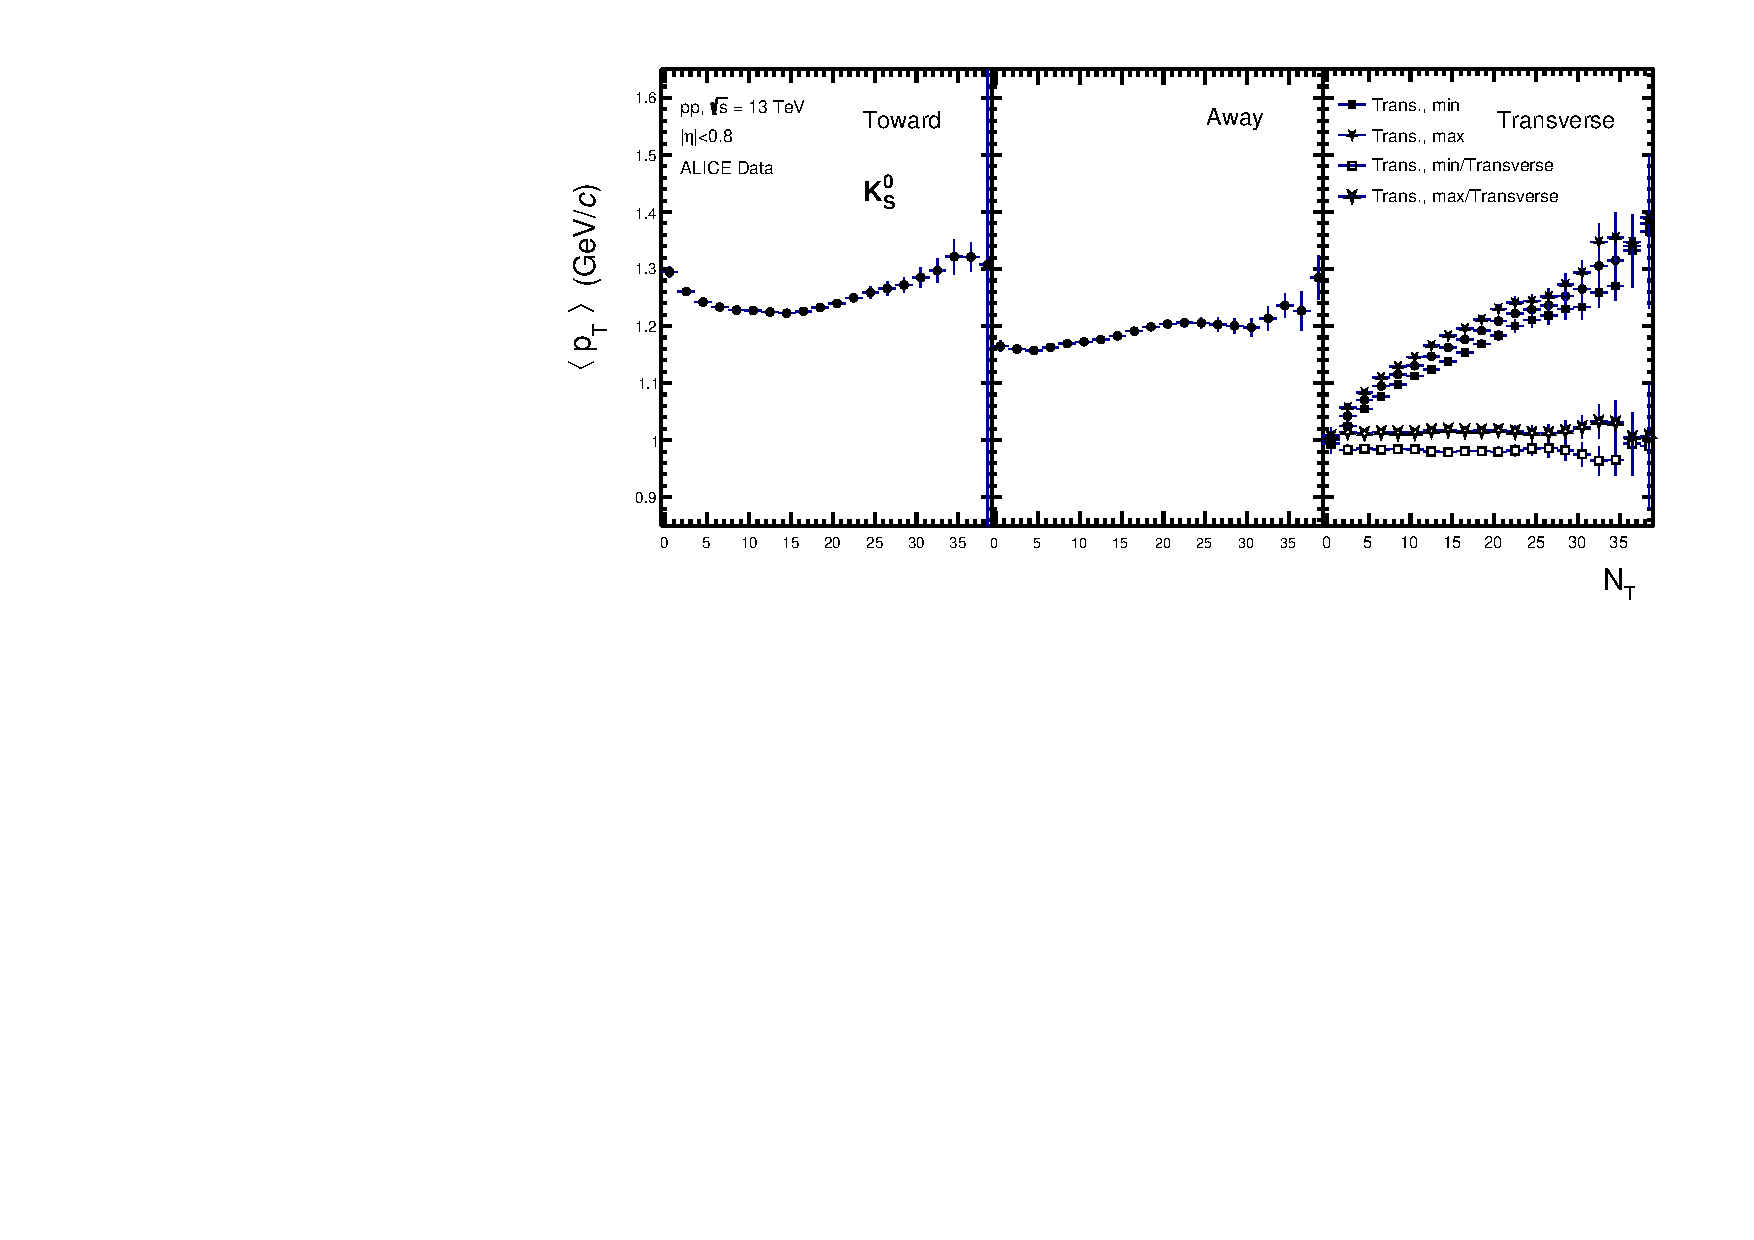
\includegraphics[width=.990\textwidth]{\imgpath/PtvNt_MeanPt_0_K0s.pdf}}\\
\subfloat[][]{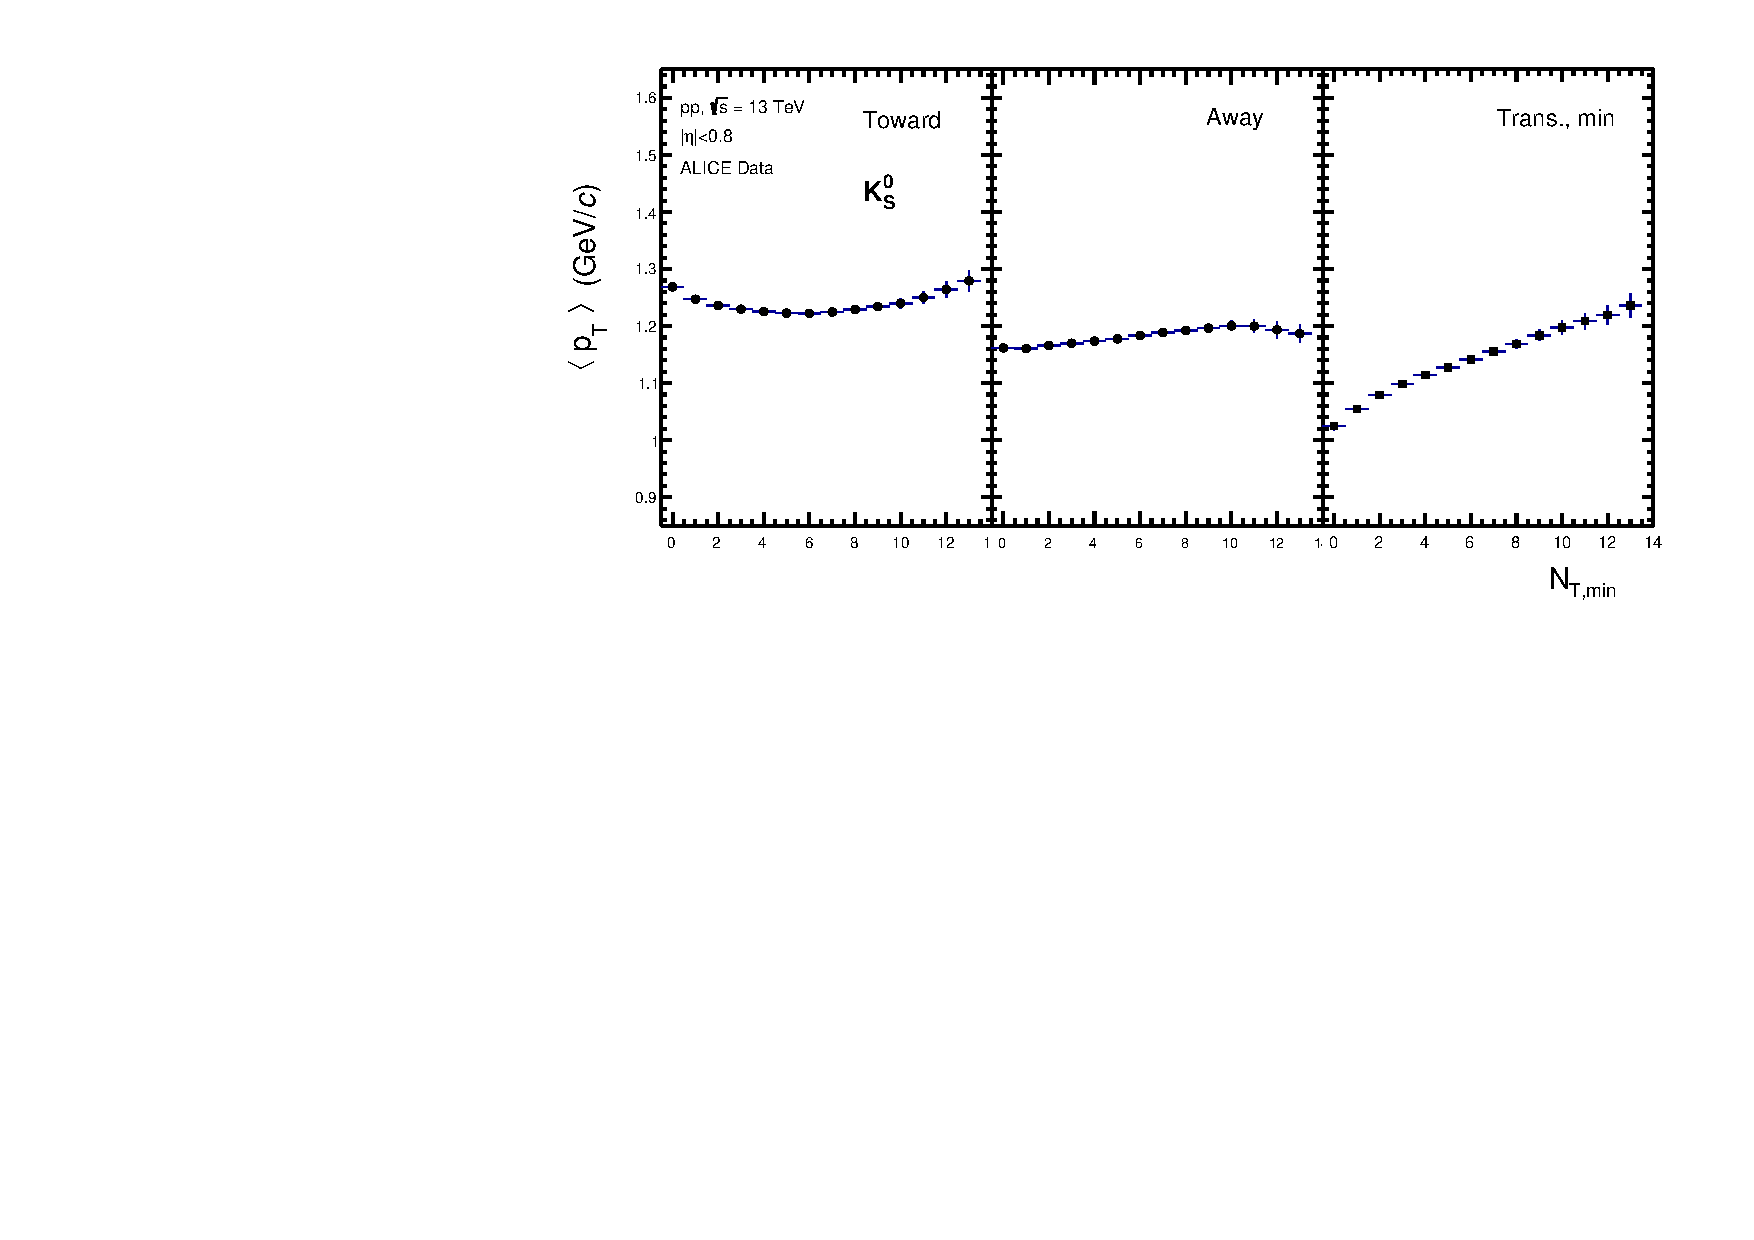
\includegraphics[width=.990\textwidth]{\imgpath/PtvNt_MeanPt_1_K0s.pdf}}\\
\subfloat[][]{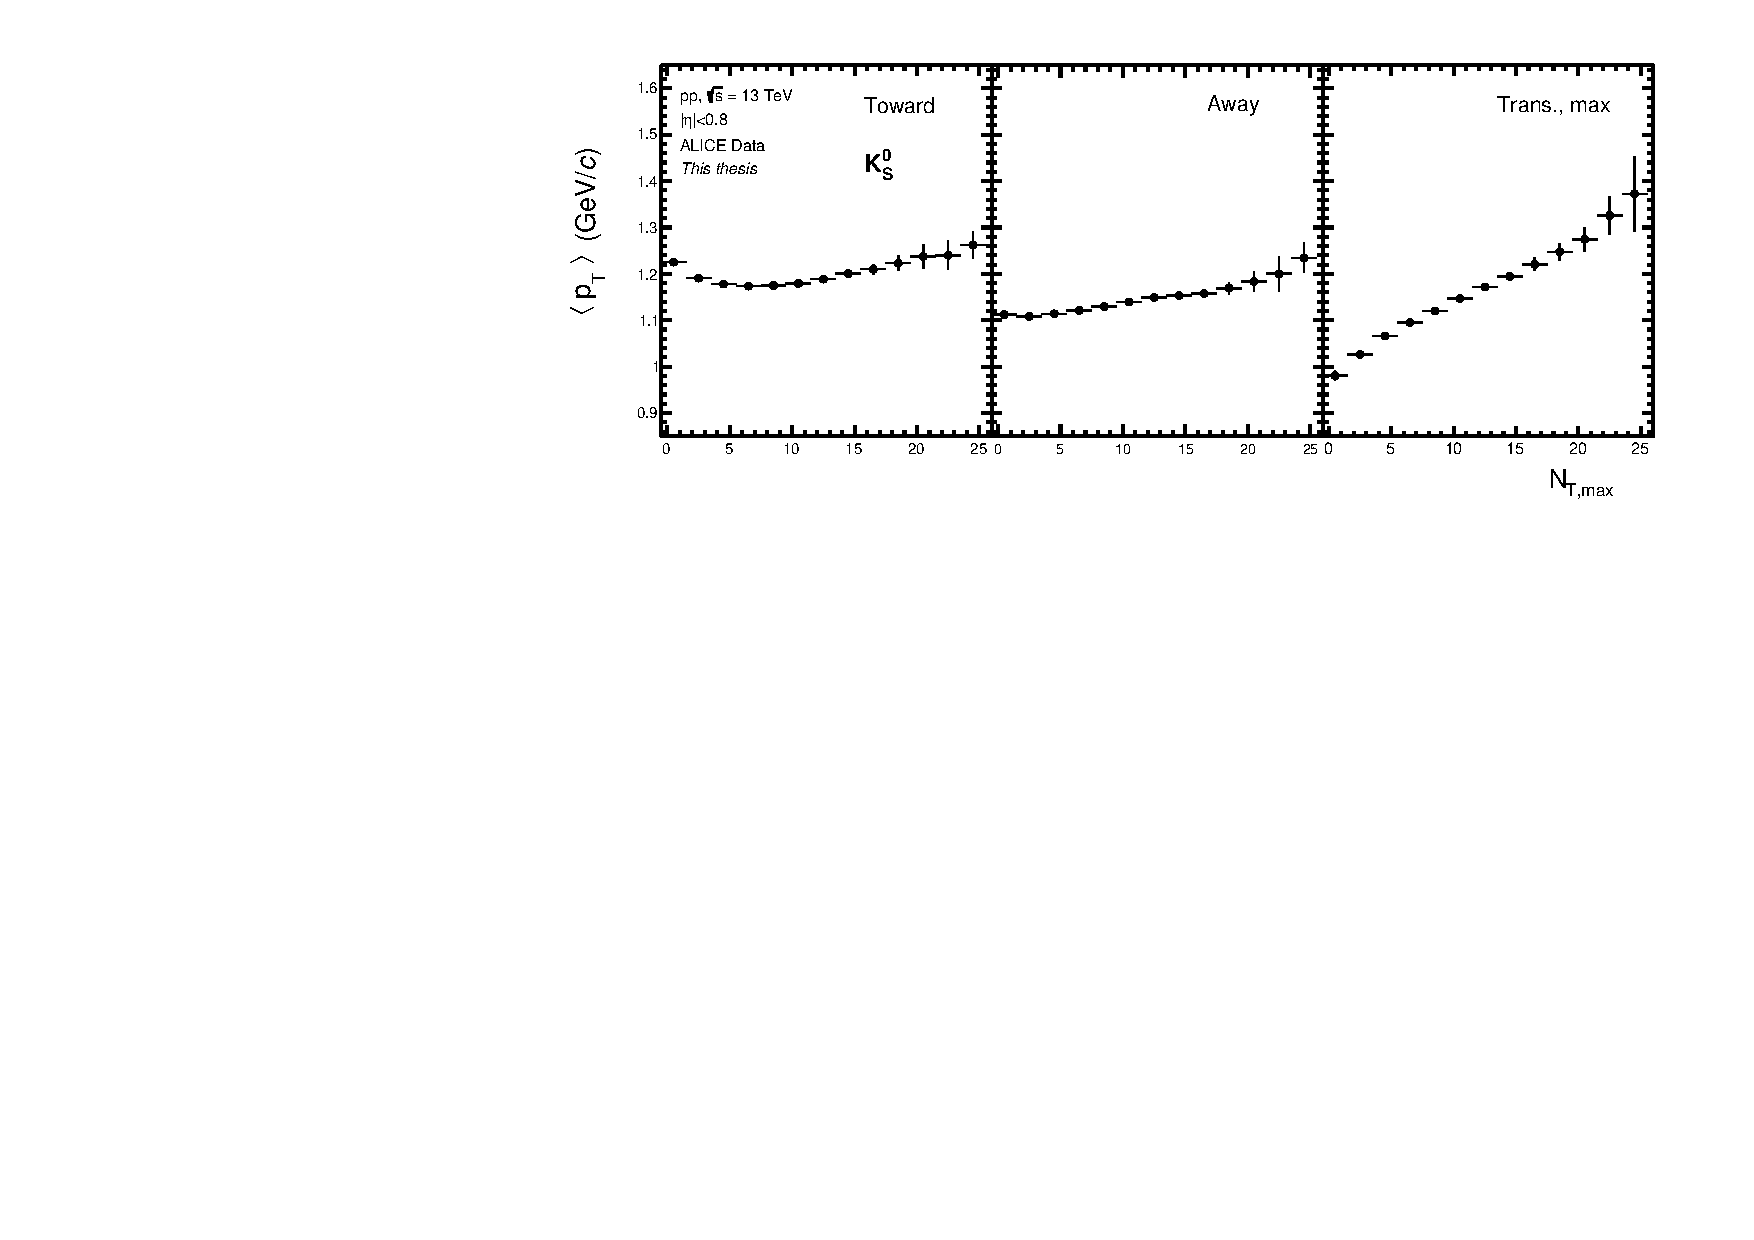
\includegraphics[width=.990\textwidth]{\imgpath/PtvNt_MeanPt_2_K0s.pdf}}\\
\caption{TBA.}
\label{fig:rt:meanptK0s}
\end{figure}

\section{Transverse momentum spectra}

TBA

\begin{figure}%
\subfloat[][]{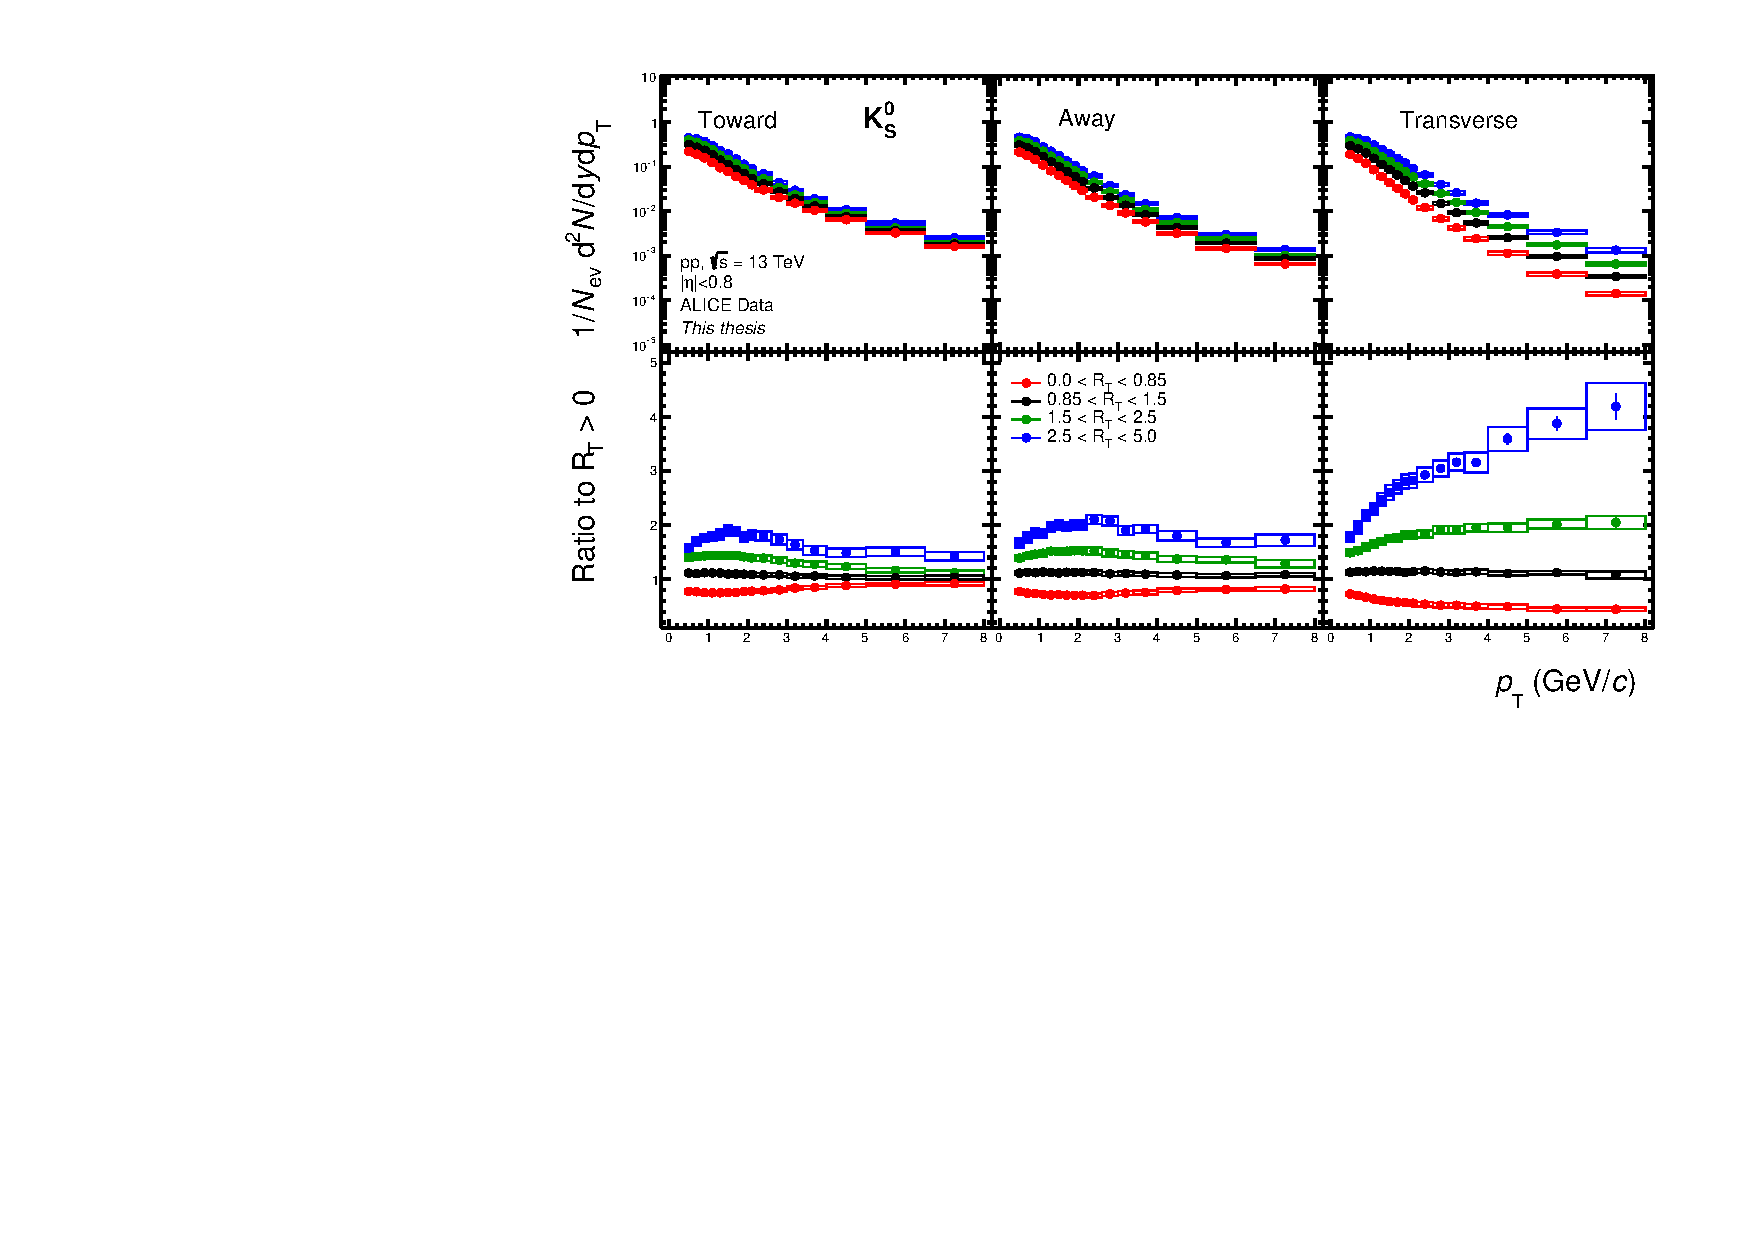
\includegraphics[width=.990\textwidth]{\imgpath/PtvRt_Pt_K0s.pdf}}\\
\subfloat[][]{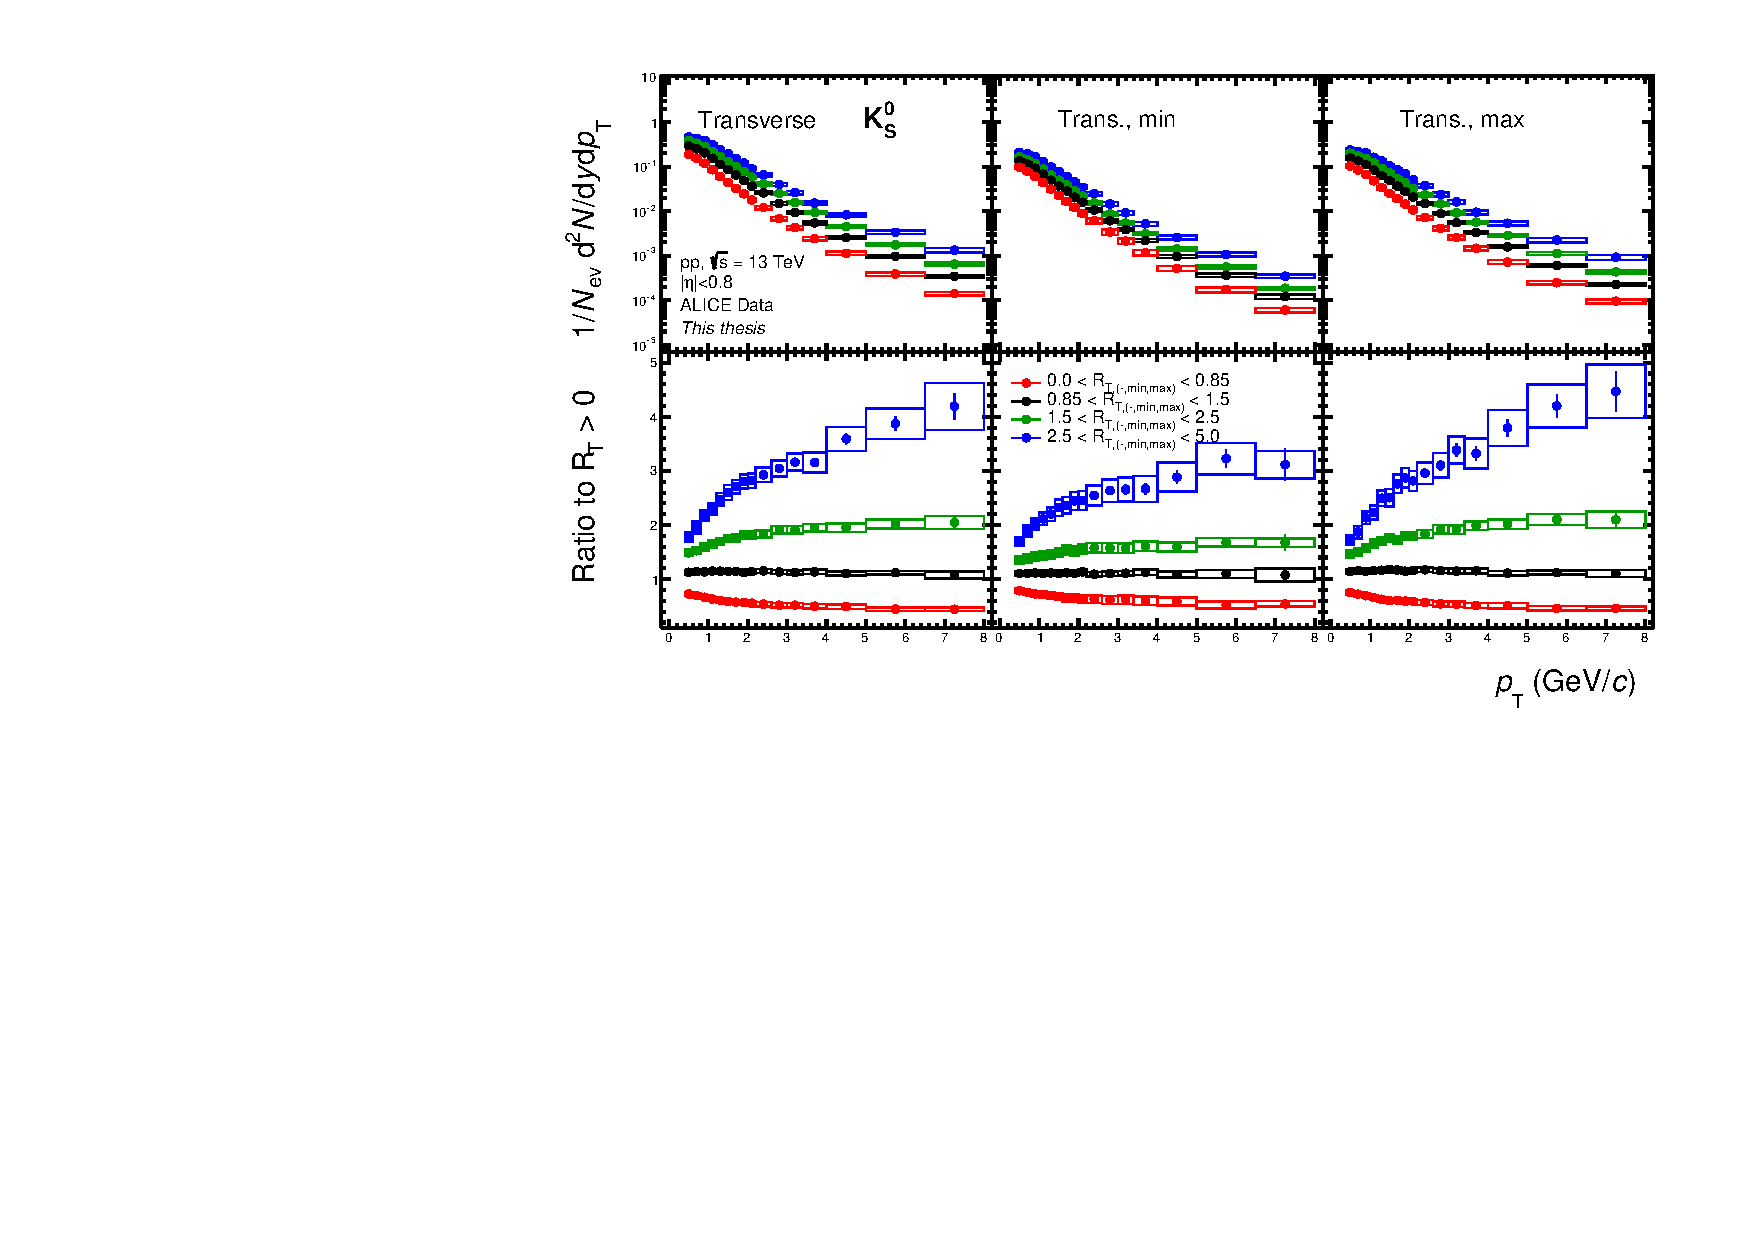
\includegraphics[width=.990\textwidth]{\imgpath/PtvRt_Pt2_K0s.pdf}}\\
\caption{The measured and fully corrected \SOPT distributions for both \textbf{(a)} \NSPD 0--1\%, \textbf{(b)} 0--10\% and \textbf{(c)} \VOM 0--1\% . The curves represent different model prediction, where the shaded area represents the statistical uncertainty of the models.}
\label{fig:rt:ptK0s}
\end{figure}


\begin{figure}%
\subfloat[][]{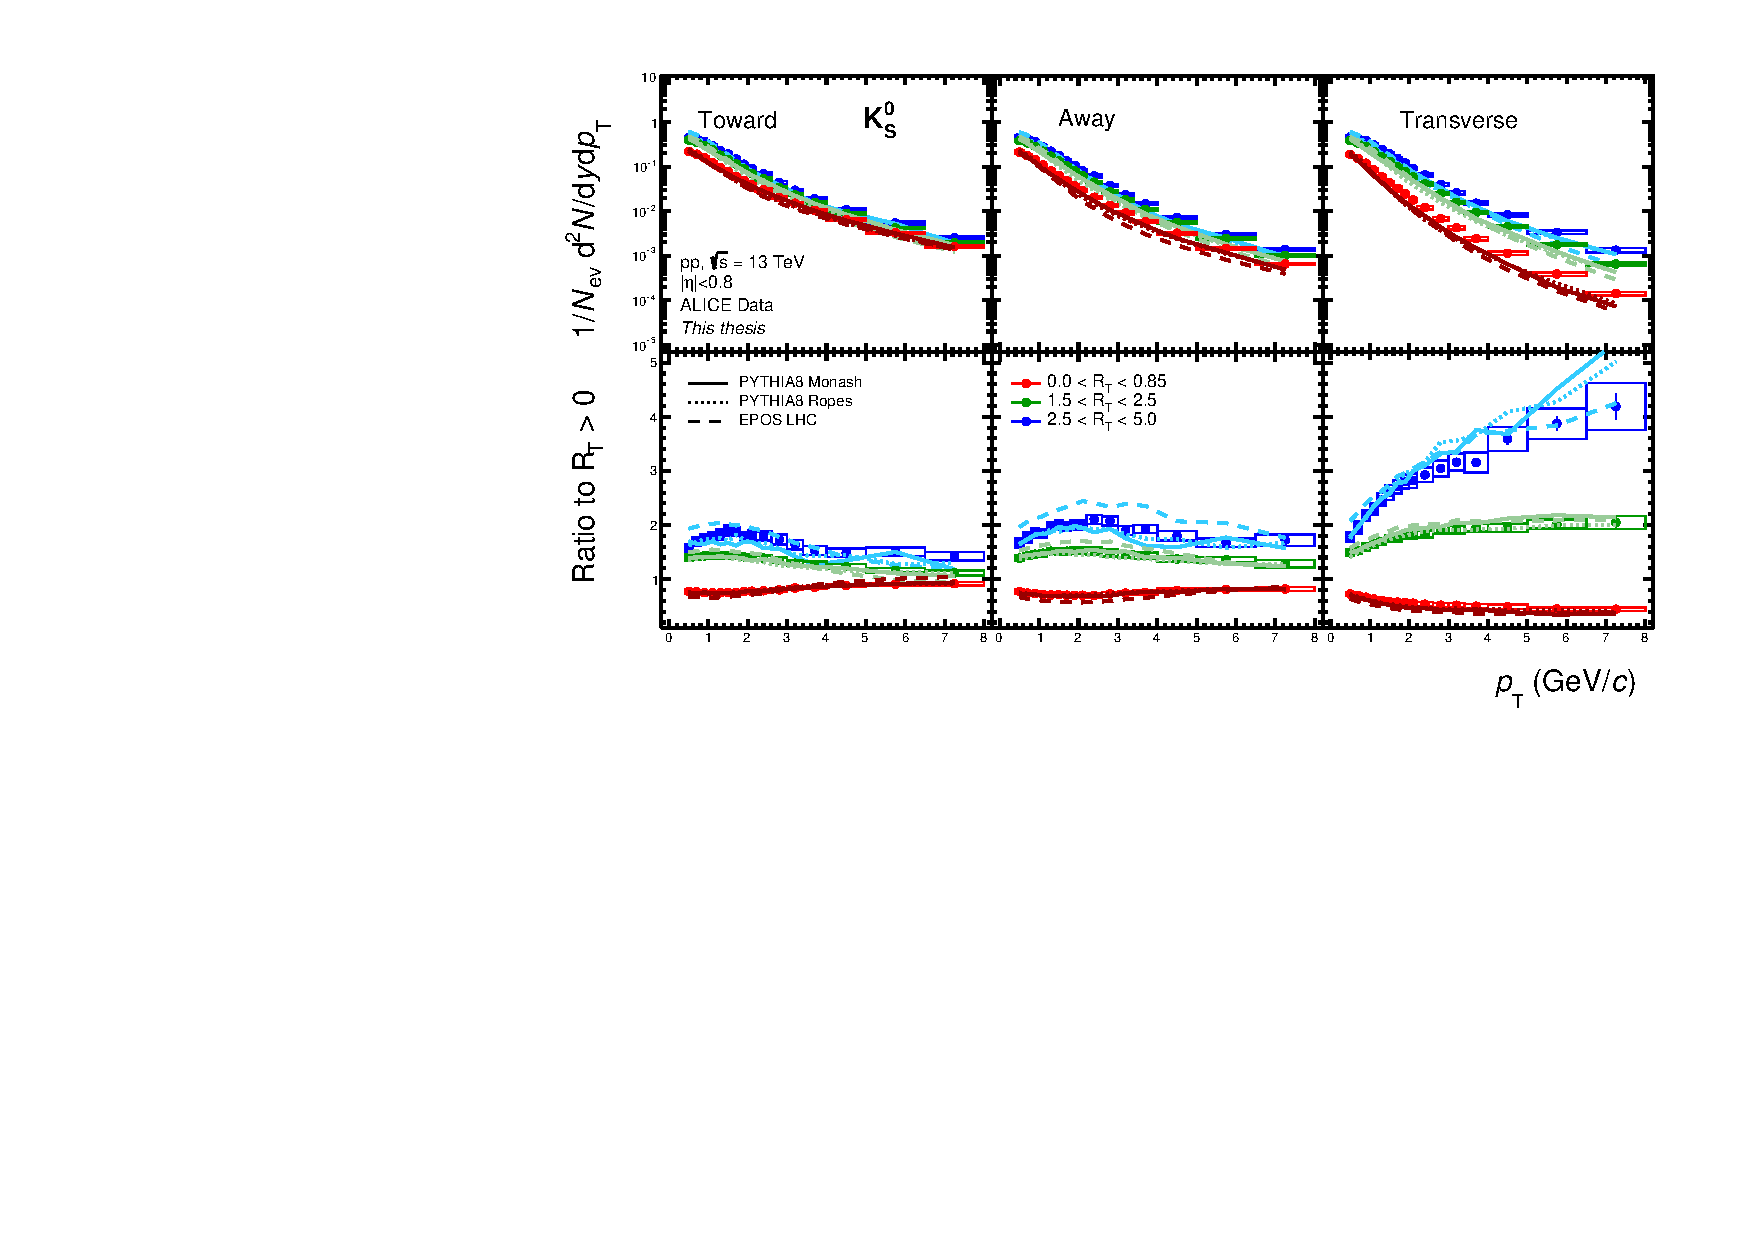
\includegraphics[width=.990\textwidth]{\imgpath/PtvRt_PtMC_K0s.pdf}}\\
\subfloat[][]{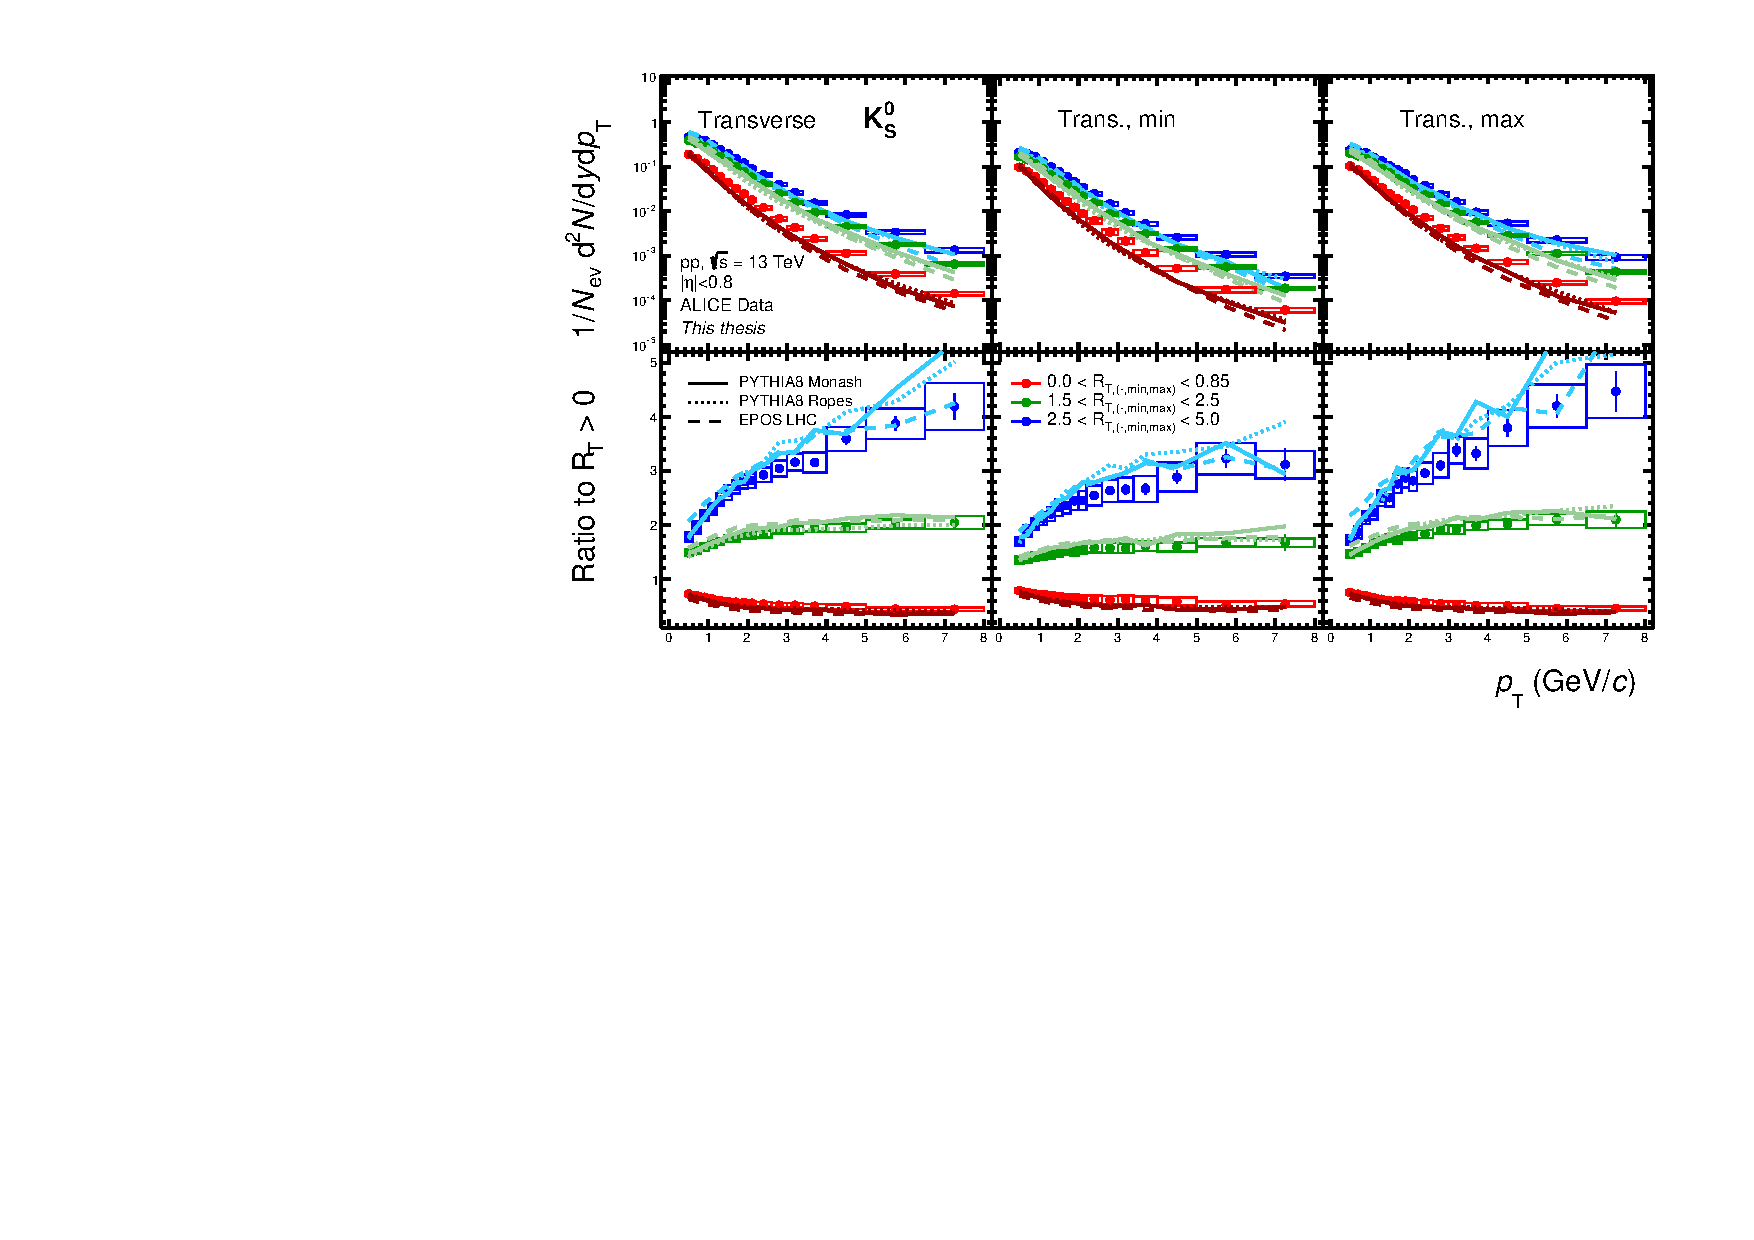
\includegraphics[width=.990\textwidth]{\imgpath/PtvRt_PtMC2_K0s.pdf}}\\
\caption{The measured and fully corrected \SOPT distributions for both \textbf{(a)} \NSPD 0--1\%, \textbf{(b)} 0--10\% and \textbf{(c)} \VOM 0--1\% . The curves represent different model prediction, where the shaded area represents the statistical uncertainty of the models.}
\label{fig:rt:ptK0sMC}
\end{figure}

\begin{figure}%
\subfloat[][]{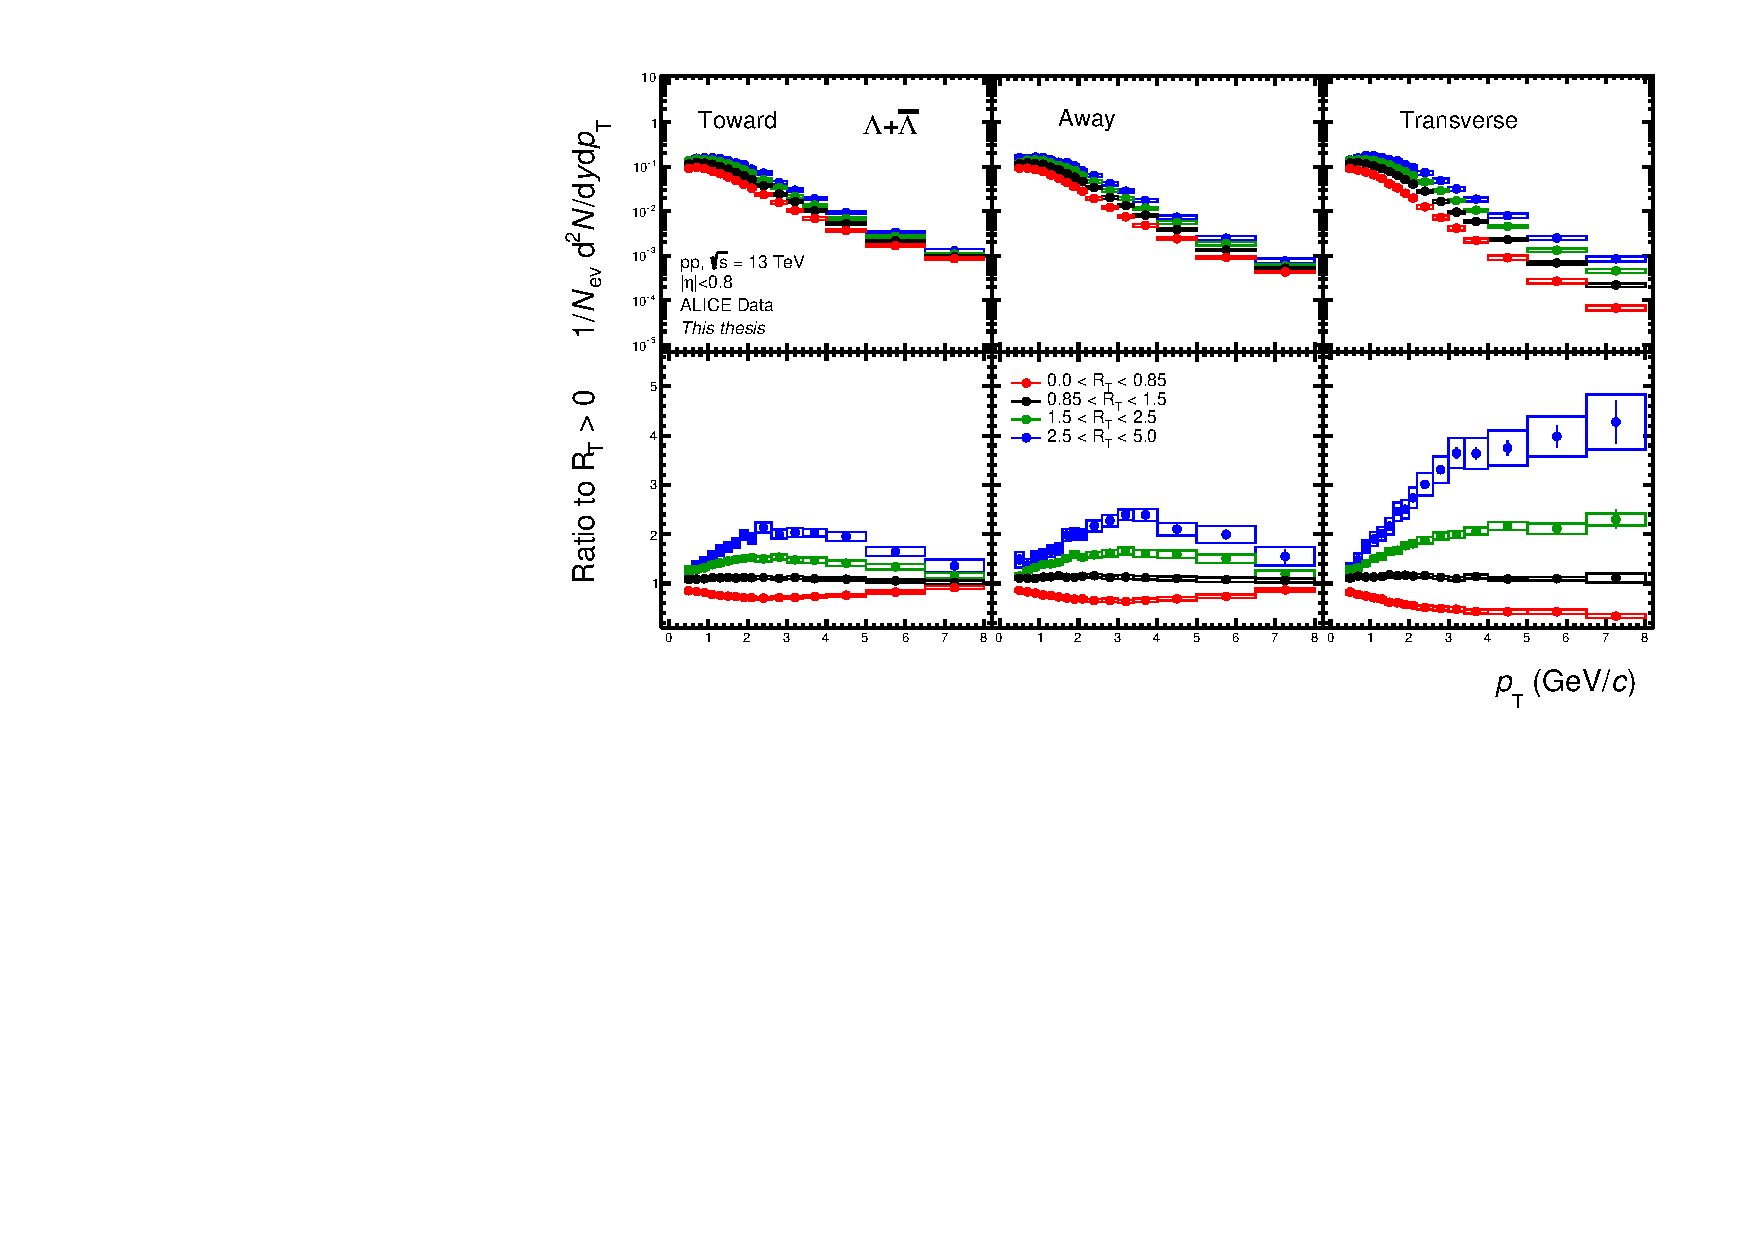
\includegraphics[width=.990\textwidth]{\imgpath/PtvRt_Pt_L.pdf}}\\
\subfloat[][]{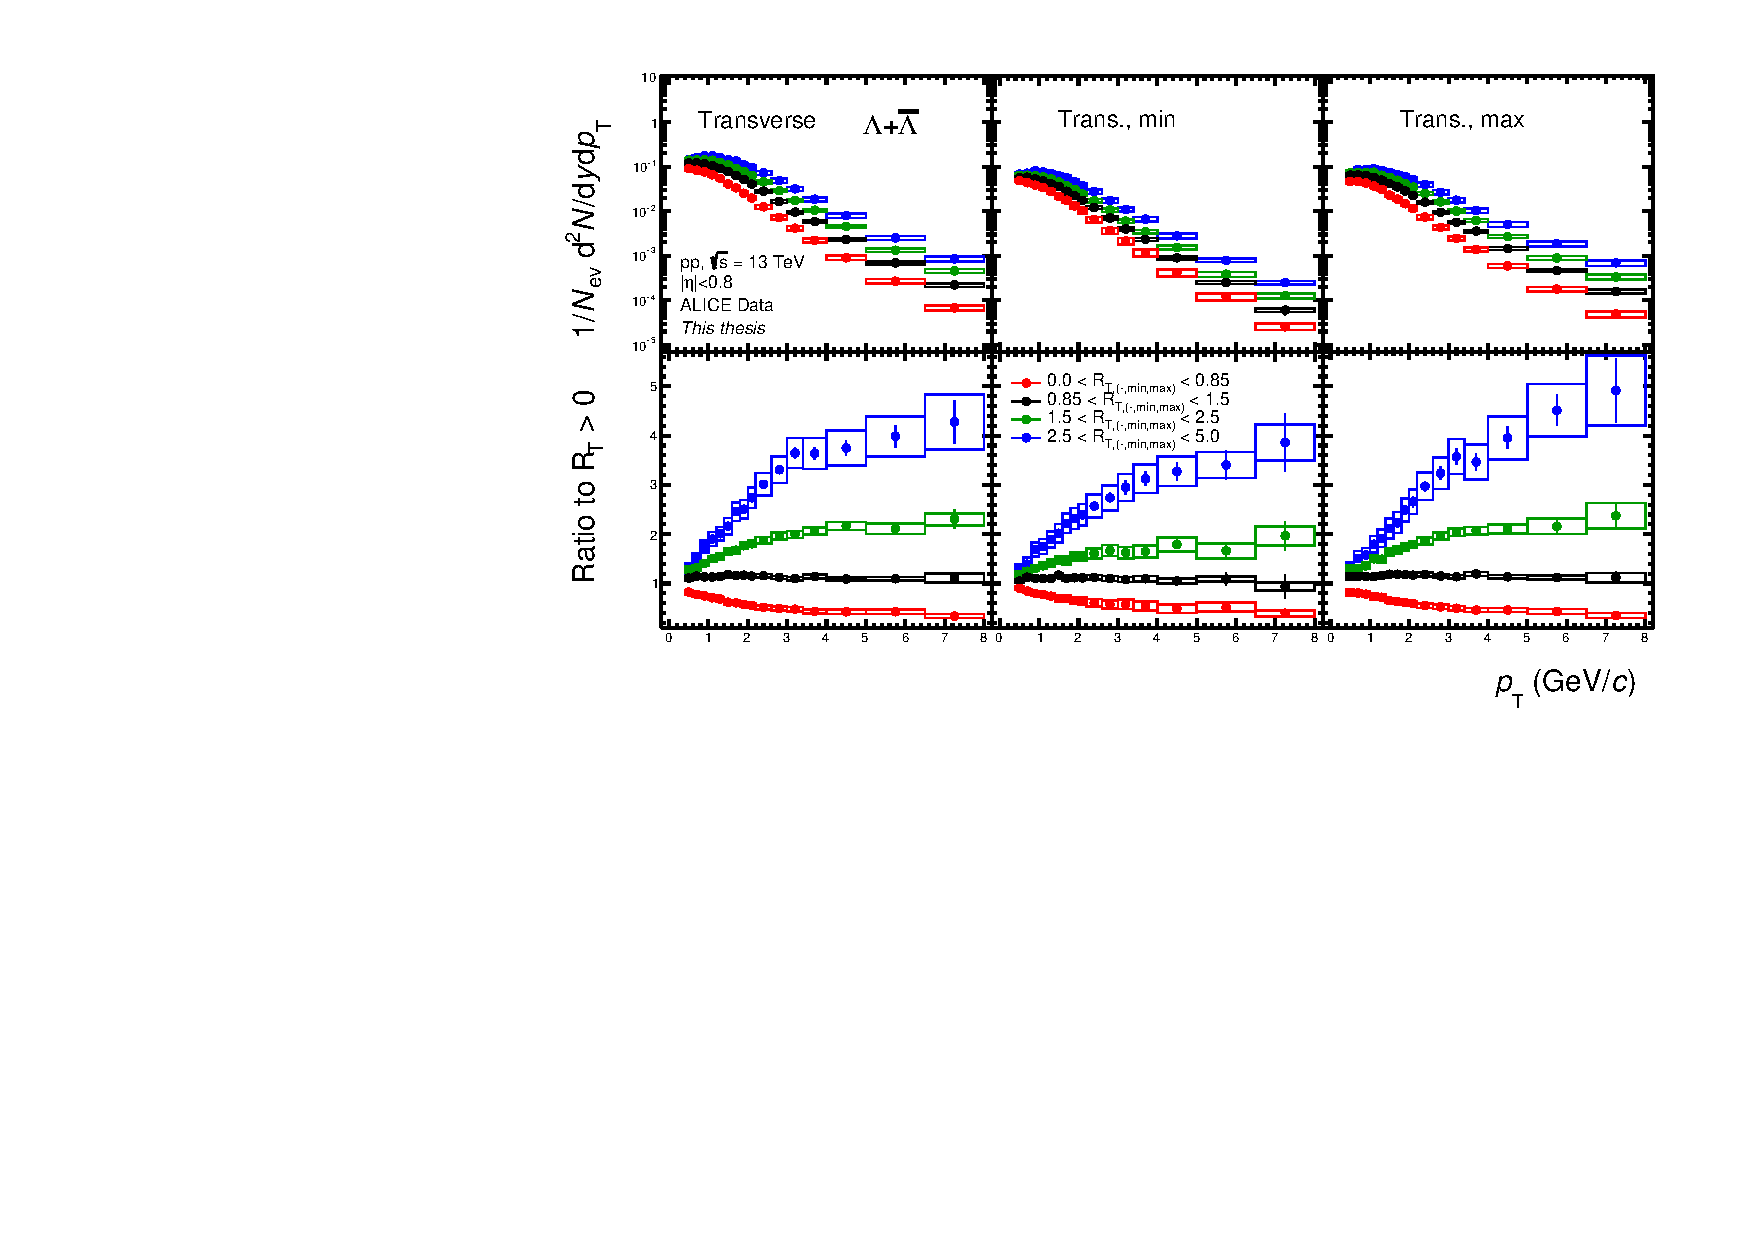
\includegraphics[width=.990\textwidth]{\imgpath/PtvRt_Pt2_L.pdf}}\\
\caption{The measured and fully corrected \SOPT distributions for both \textbf{(a)} \NSPD 0--1\%, \textbf{(b)} 0--10\% and \textbf{(c)} \VOM 0--1\% . The curves represent different model prediction, where the shaded area represents the statistical uncertainty of the models.}
\label{fig:rt:ptK0s}
\end{figure}


\begin{figure}%
\subfloat[][]{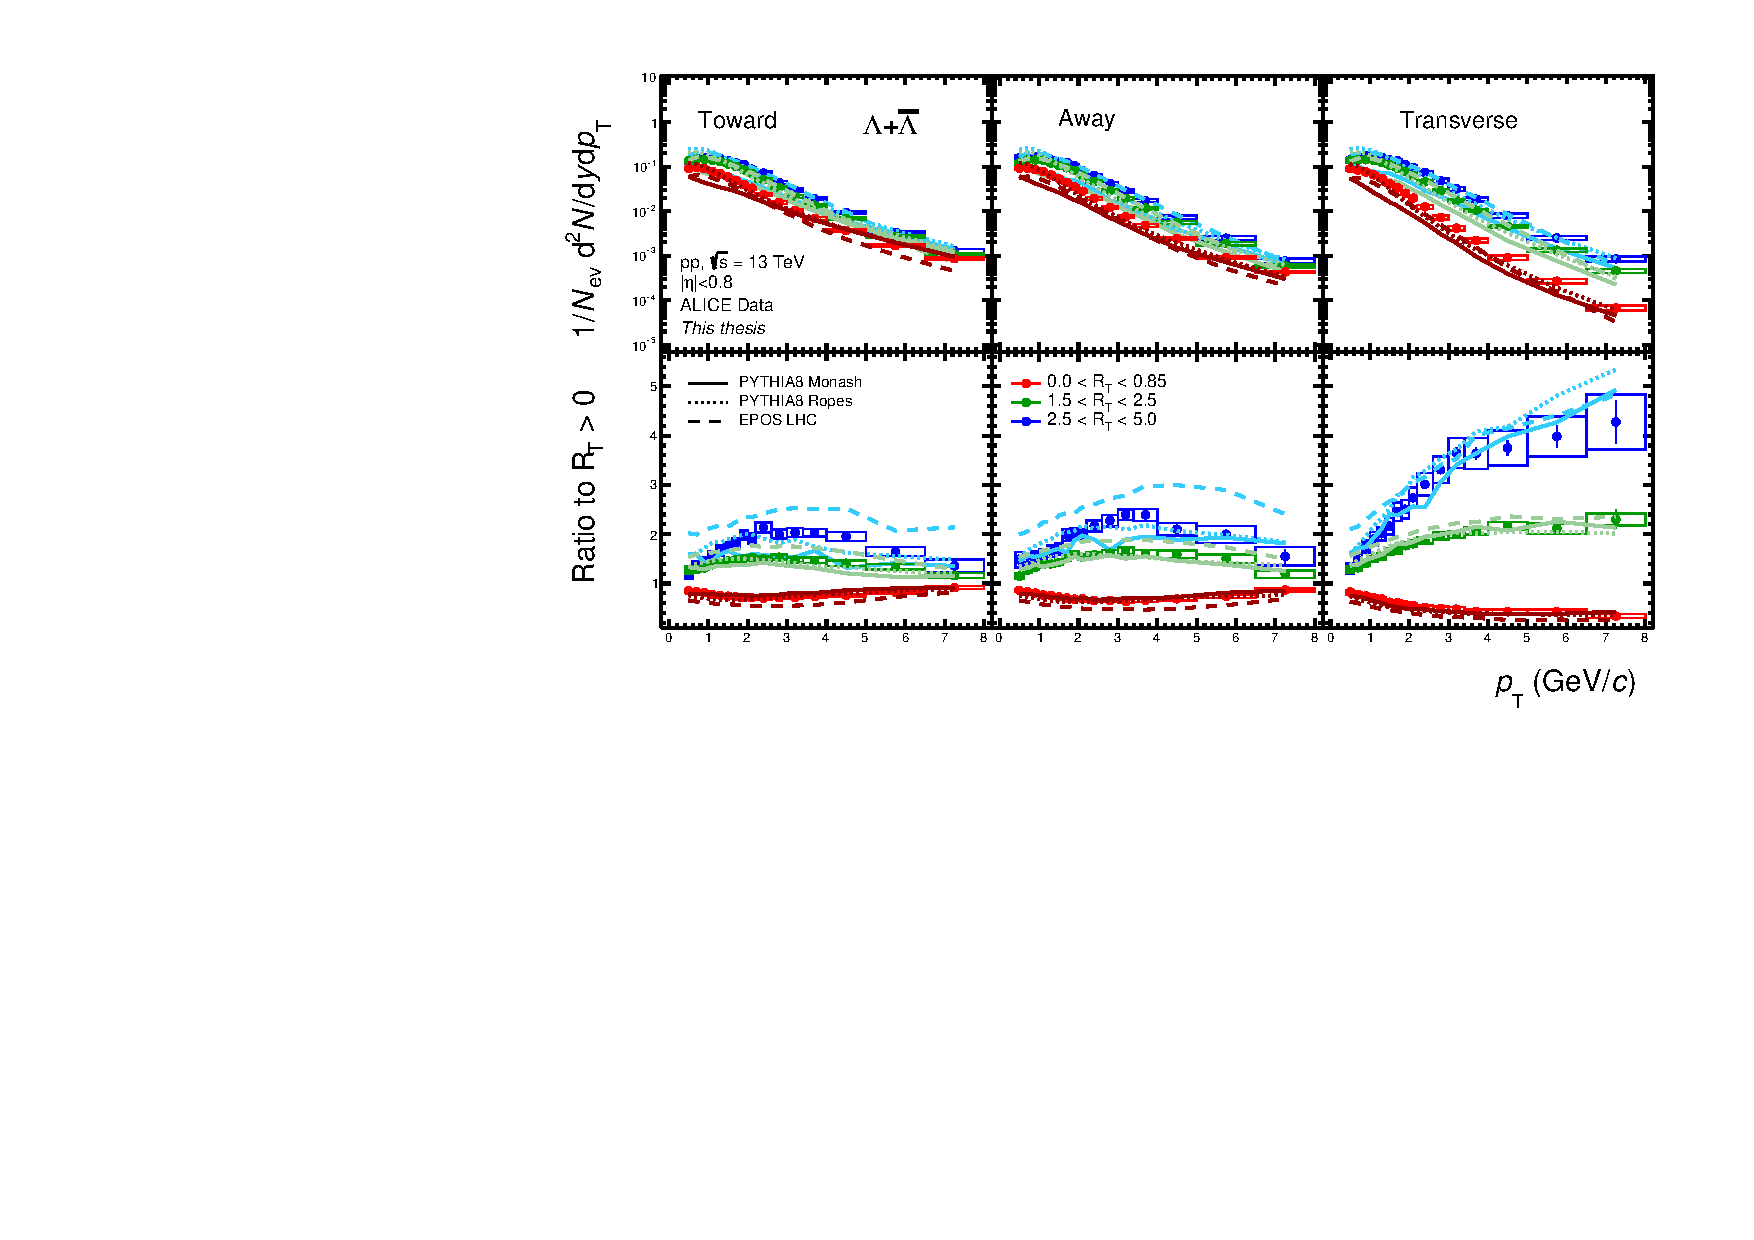
\includegraphics[width=.990\textwidth]{\imgpath/PtvRt_PtMC_L.pdf}}\\
\subfloat[][]{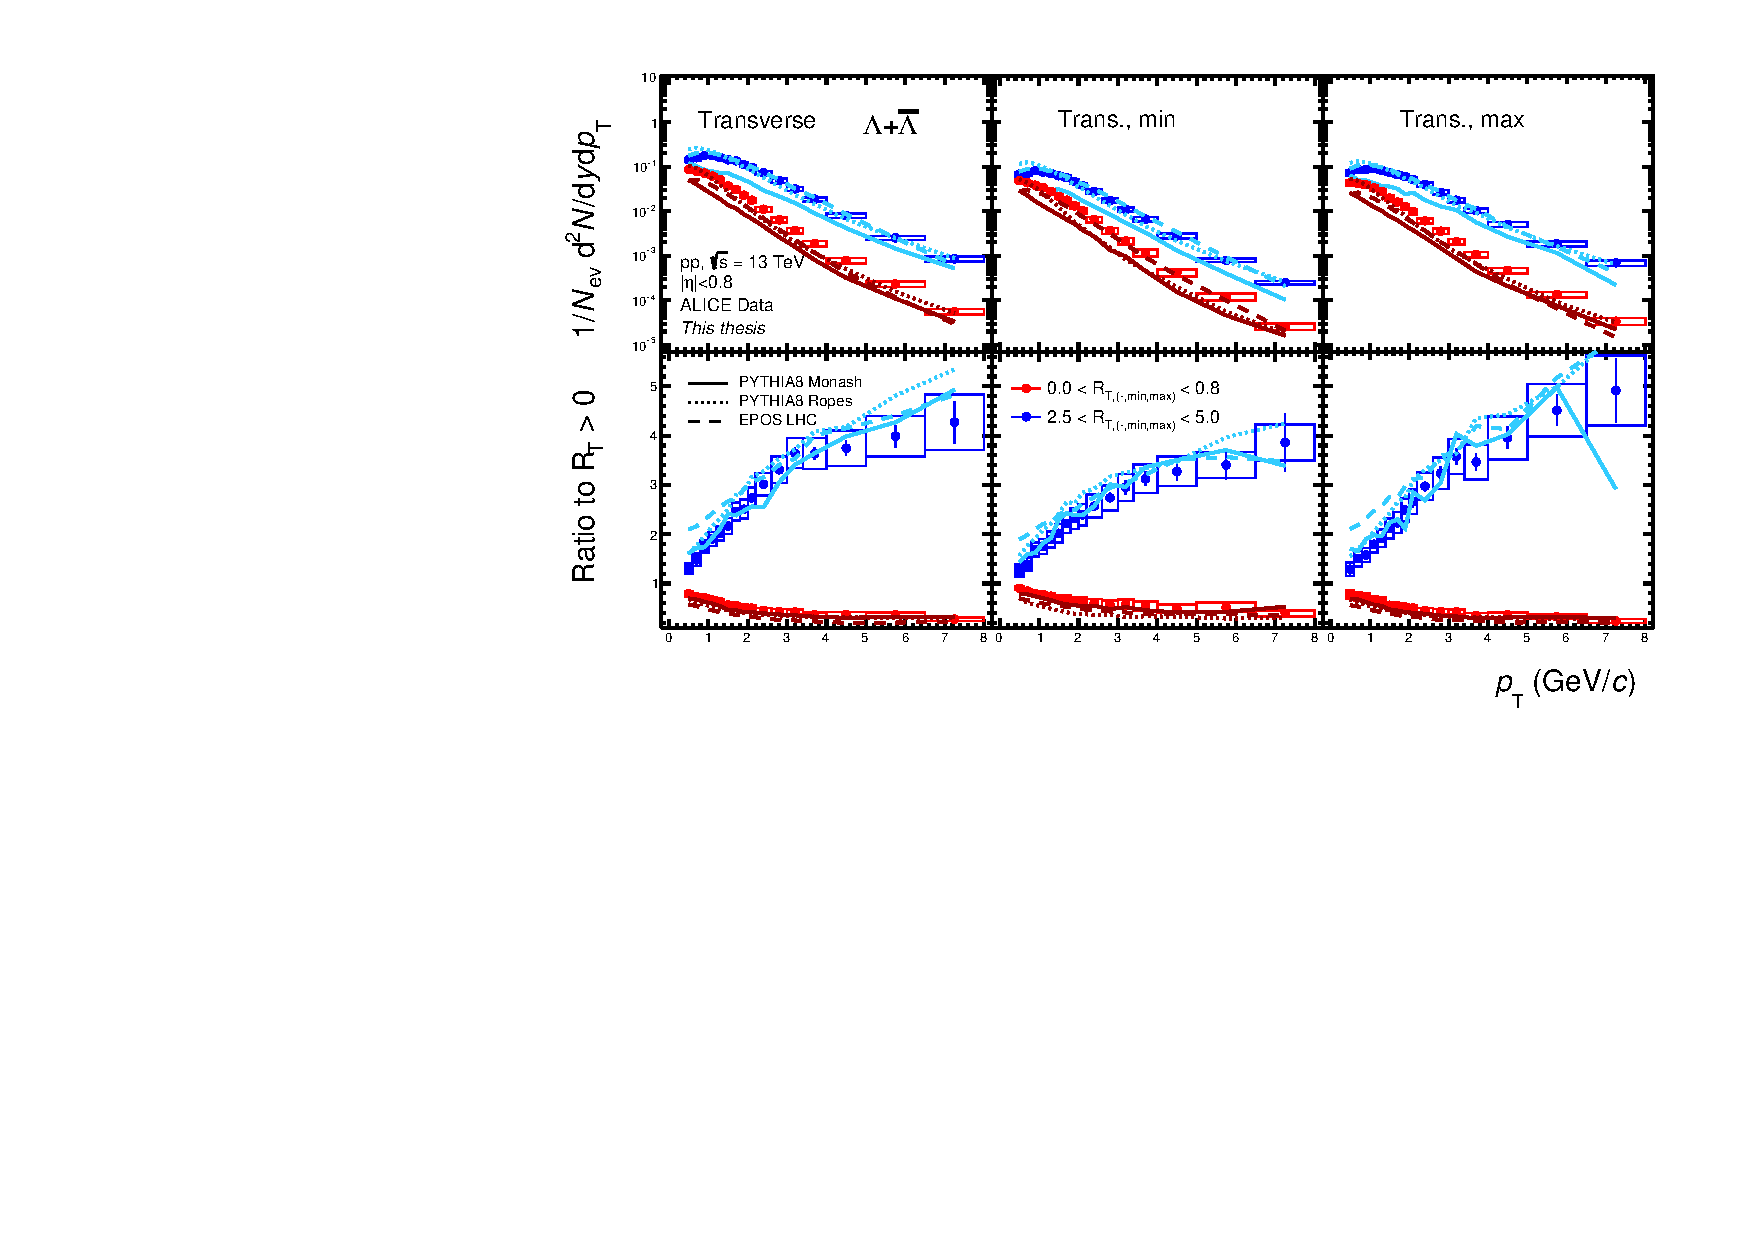
\includegraphics[width=.990\textwidth]{\imgpath/PtvRt_PtMC2_L.pdf}}\\
\caption{The measured and fully corrected \SOPT distributions for both \textbf{(a)} \NSPD 0--1\%, \textbf{(b)} 0--10\% and \textbf{(c)} \VOM 0--1\% . The curves represent different model prediction, where the shaded area represents the statistical uncertainty of the models.}
\label{fig:rt:ptK0sMC}
\end{figure}

\section{Baryon-to-meson ratio}

TBA

\begin{figure}%
\subfloat[][]{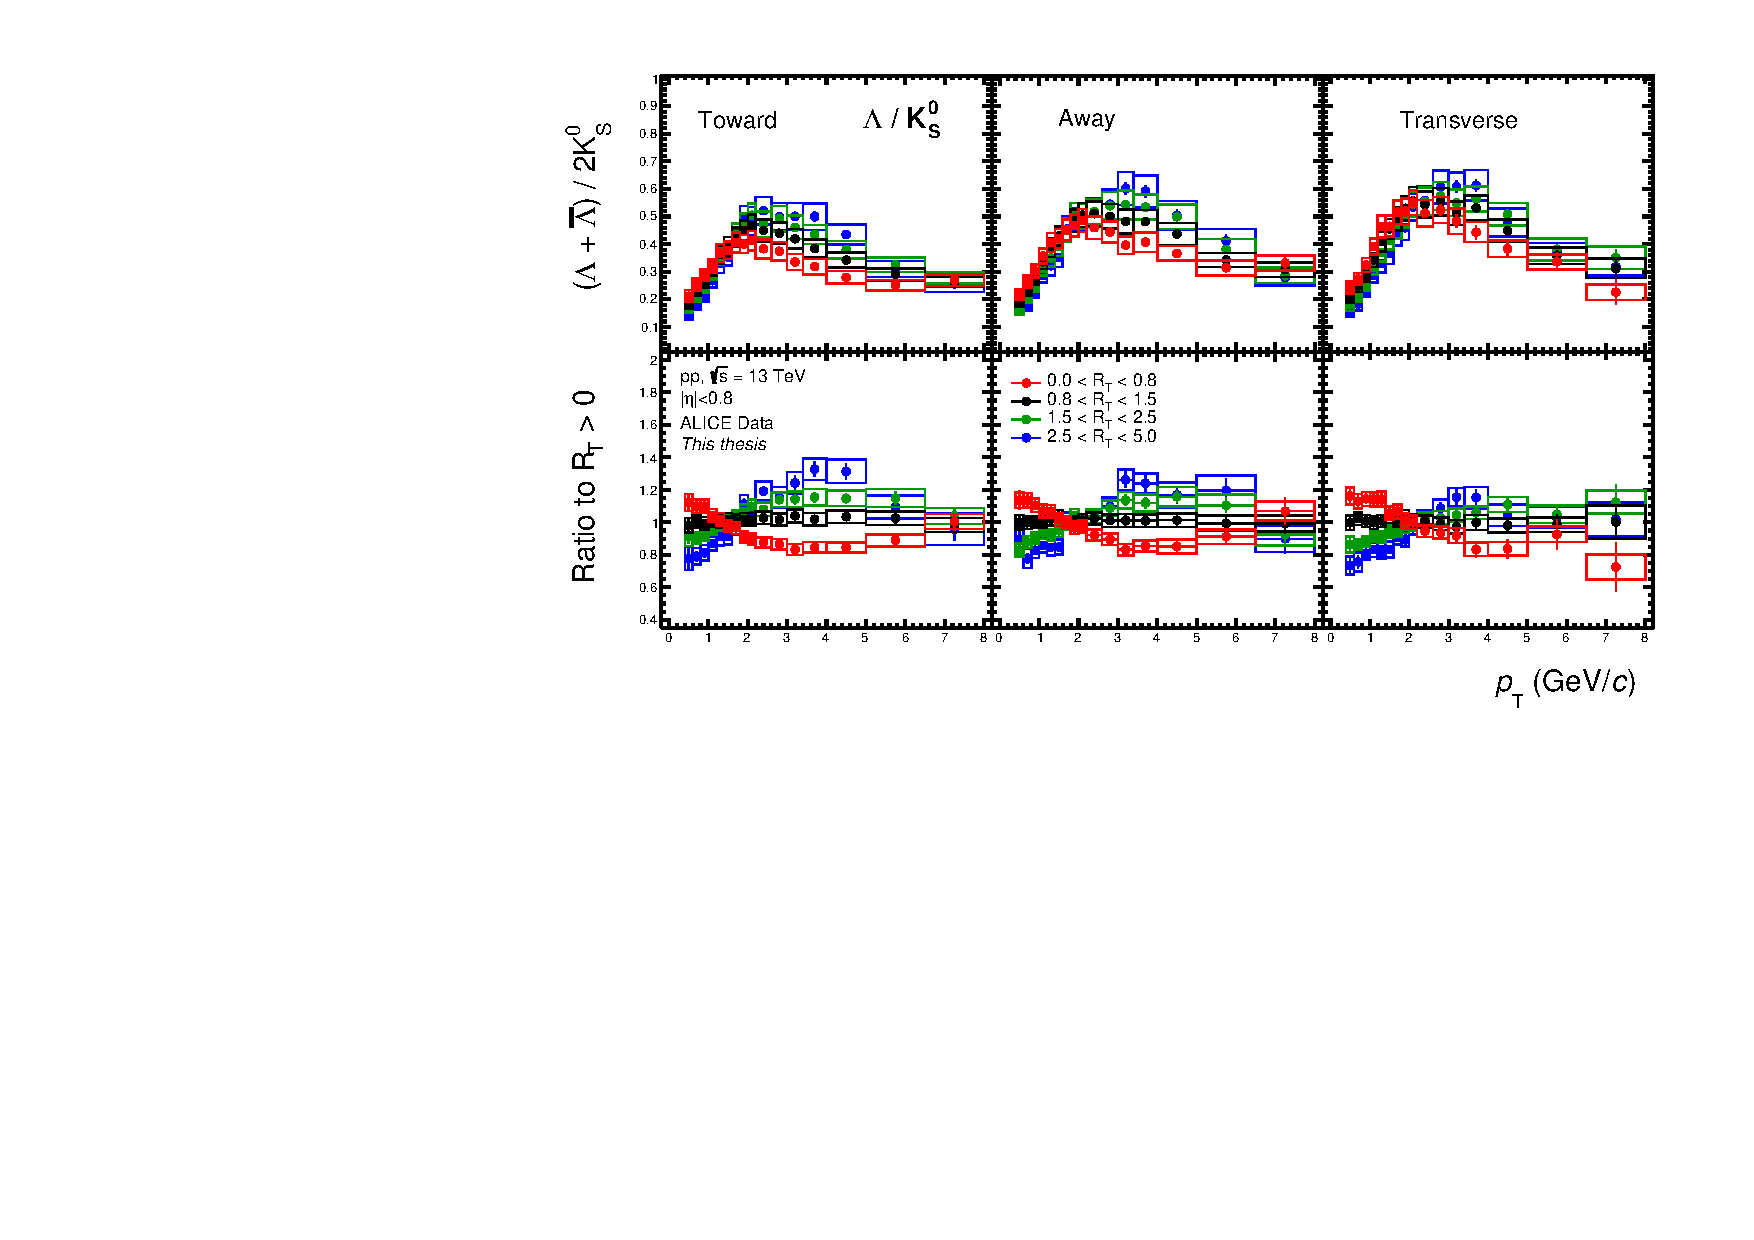
\includegraphics[width=.990\textwidth]{\imgpath/PtvRt_LtoK_K0s.pdf}}\\
\subfloat[][]{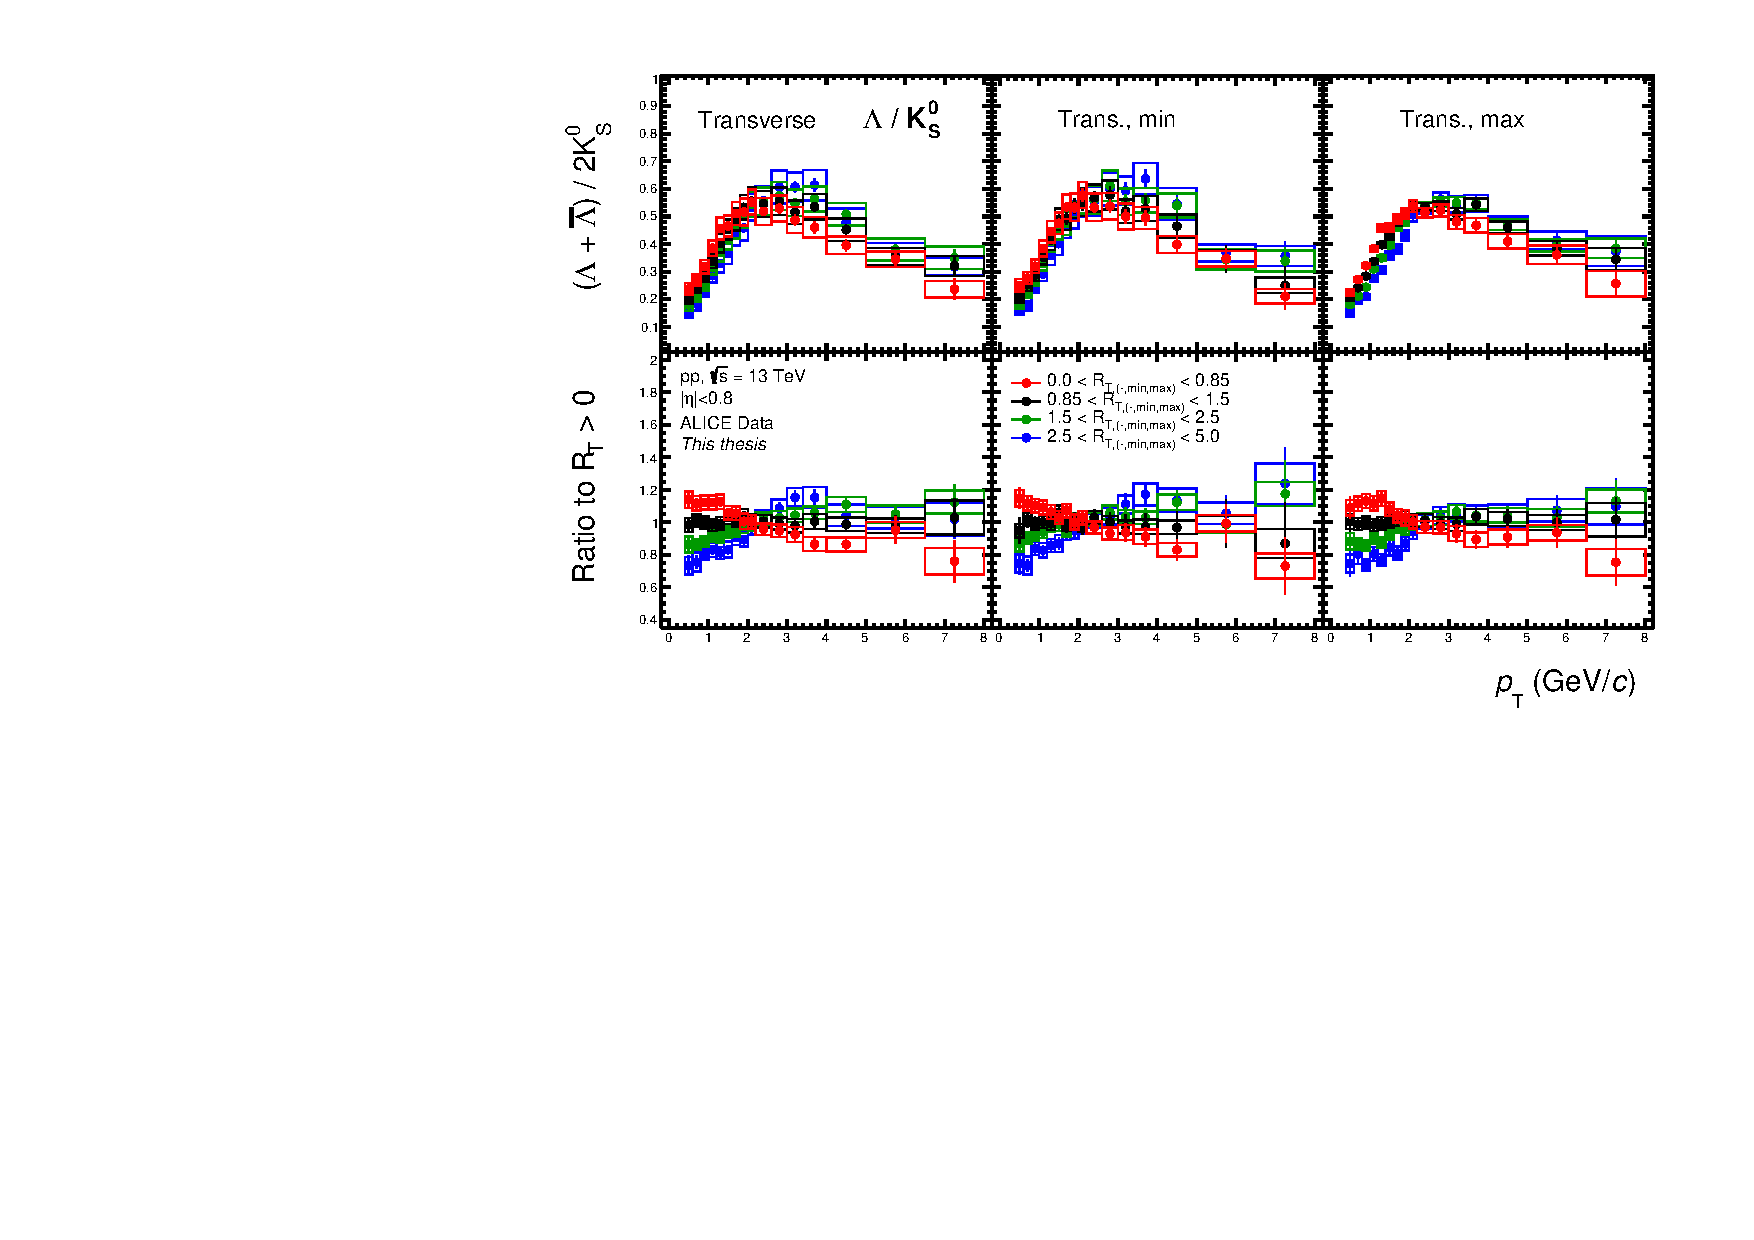
\includegraphics[width=.990\textwidth]{\imgpath/PtvRt_LtoK2_K0s.pdf}}\\
\caption{The measured and fully corrected \SOPT distributions for both \textbf{(a)} \NSPD 0--1\%, \textbf{(b)} 0--10\% and \textbf{(c)} \VOM 0--1\% . The curves represent different model prediction, where the shaded area represents the statistical uncertainty of the models.}
\label{fig:rt:LtoK}
\end{figure}


\begin{figure}%
\subfloat[][]{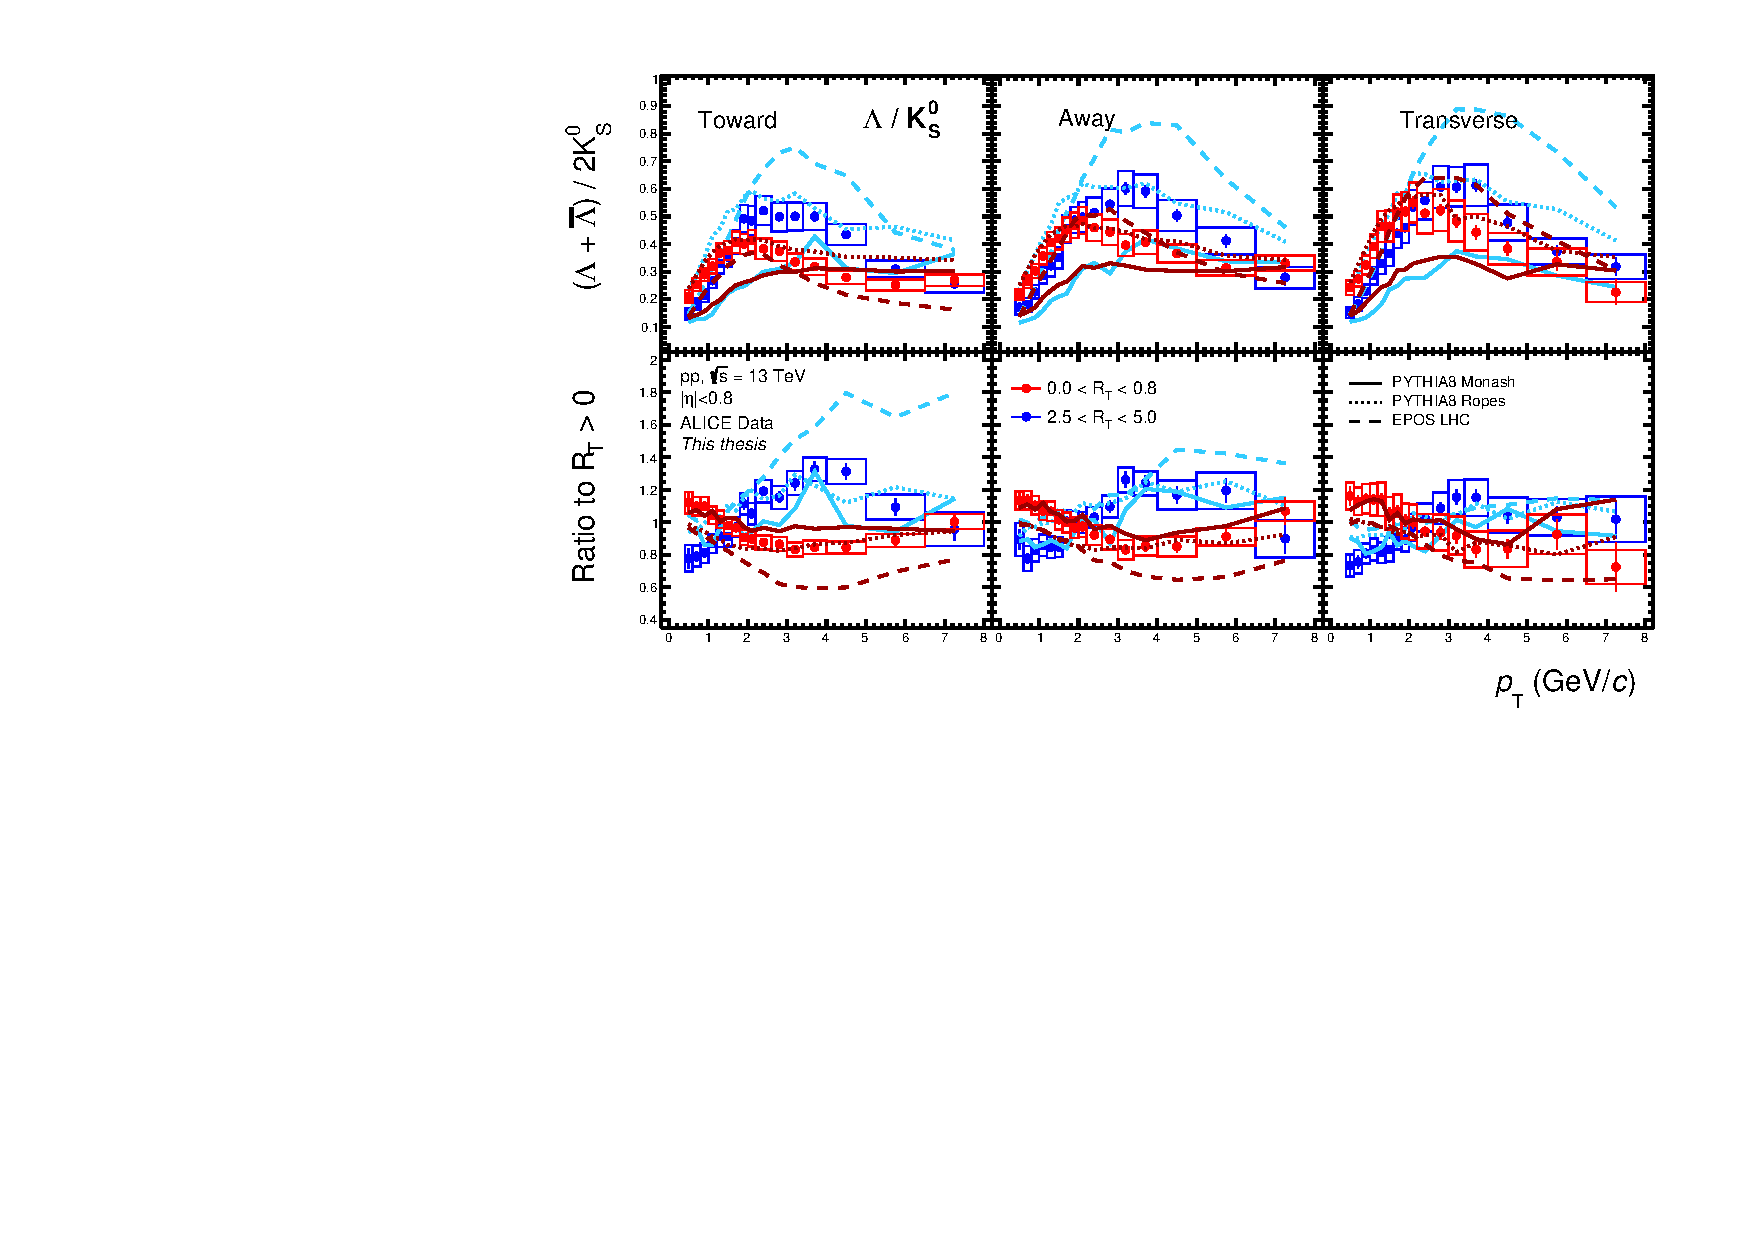
\includegraphics[width=.990\textwidth]{\imgpath/PtvRt_LtoKMC_K0s.pdf}}\\
\subfloat[][]{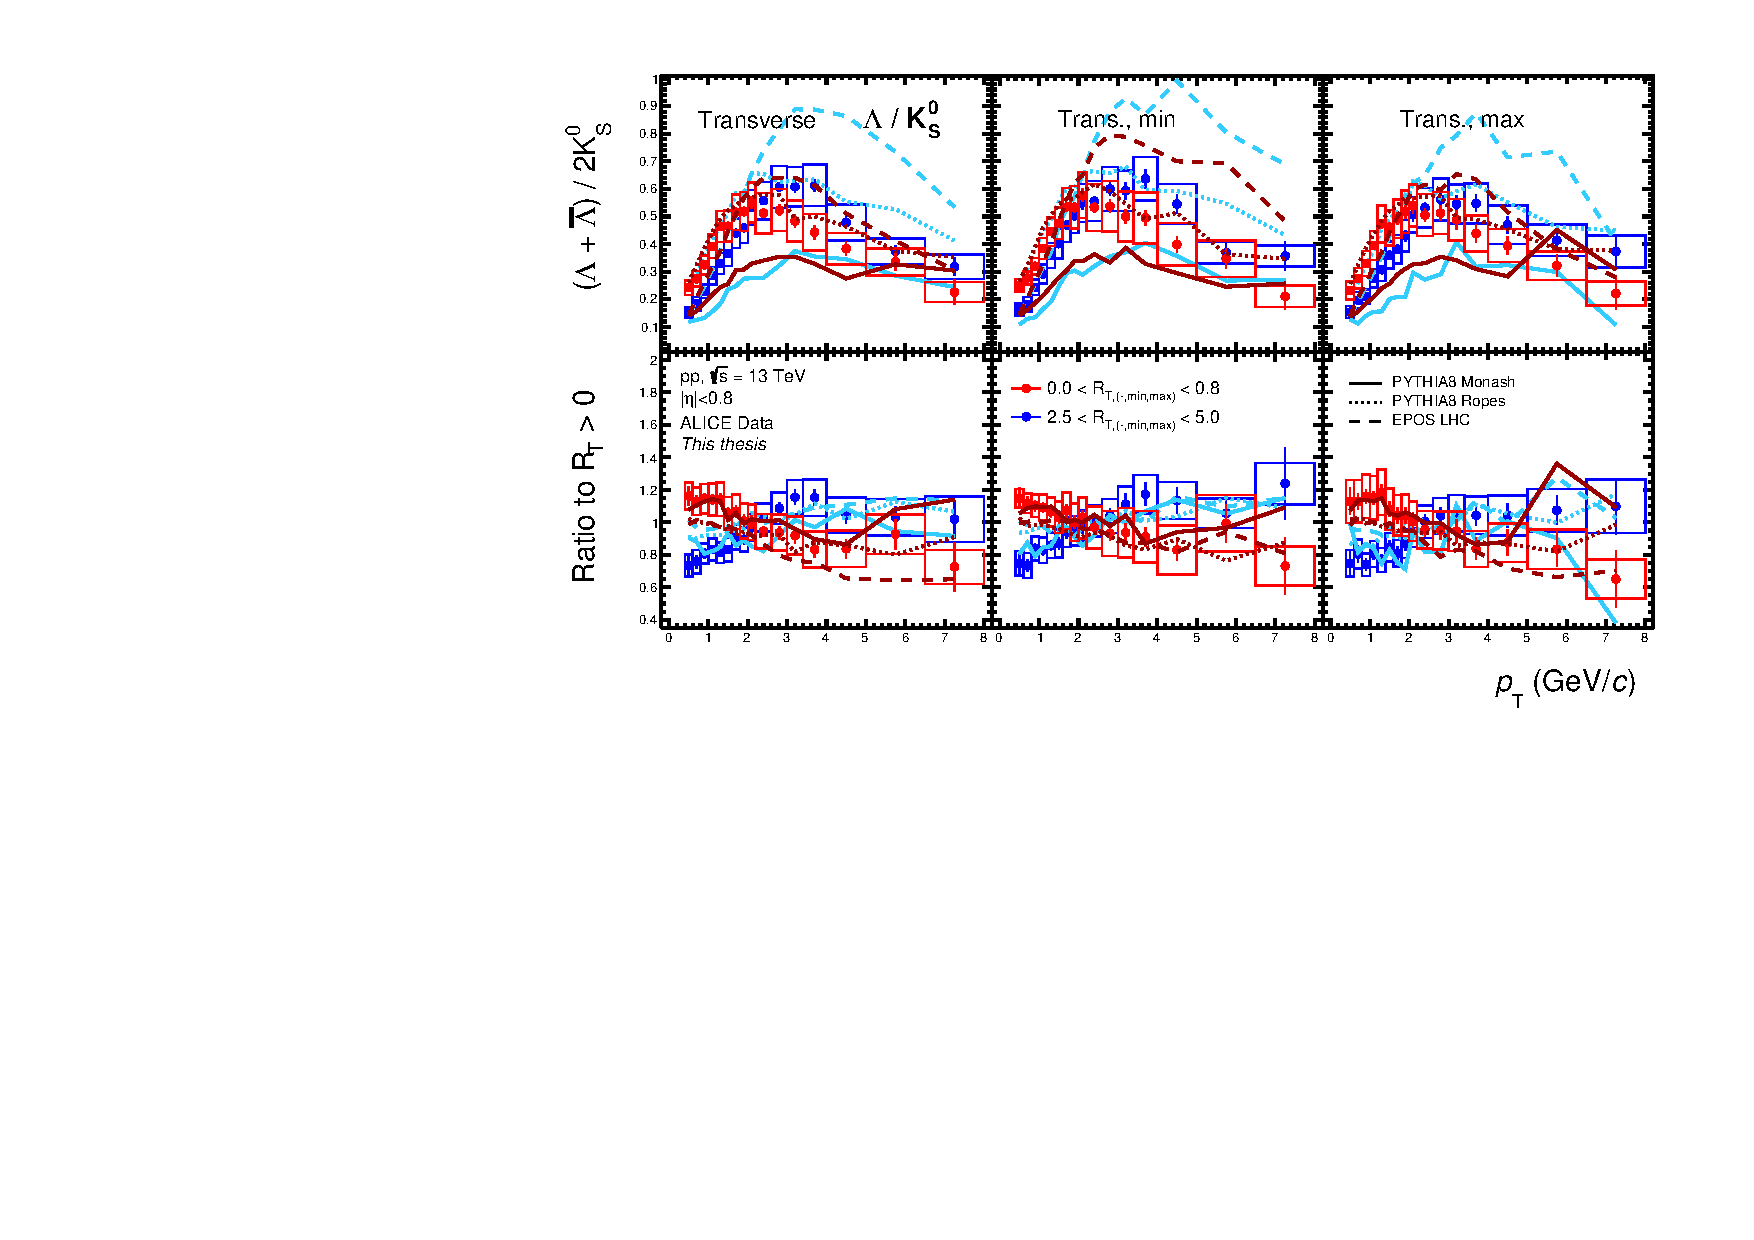
\includegraphics[width=.990\textwidth]{\imgpath/PtvRt_LtoKMC2_K0s.pdf}}\\
\caption{The measured and fully corrected \SOPT distributions for both \textbf{(a)} \NSPD 0--1\%, \textbf{(b)} 0--10\% and \textbf{(c)} \VOM 0--1\% . The curves represent different model prediction, where the shaded area represents the statistical uncertainty of the models.}
\label{fig:rt:LtoKMC}
\end{figure}

\begin{figure}%
\subfloat[][]{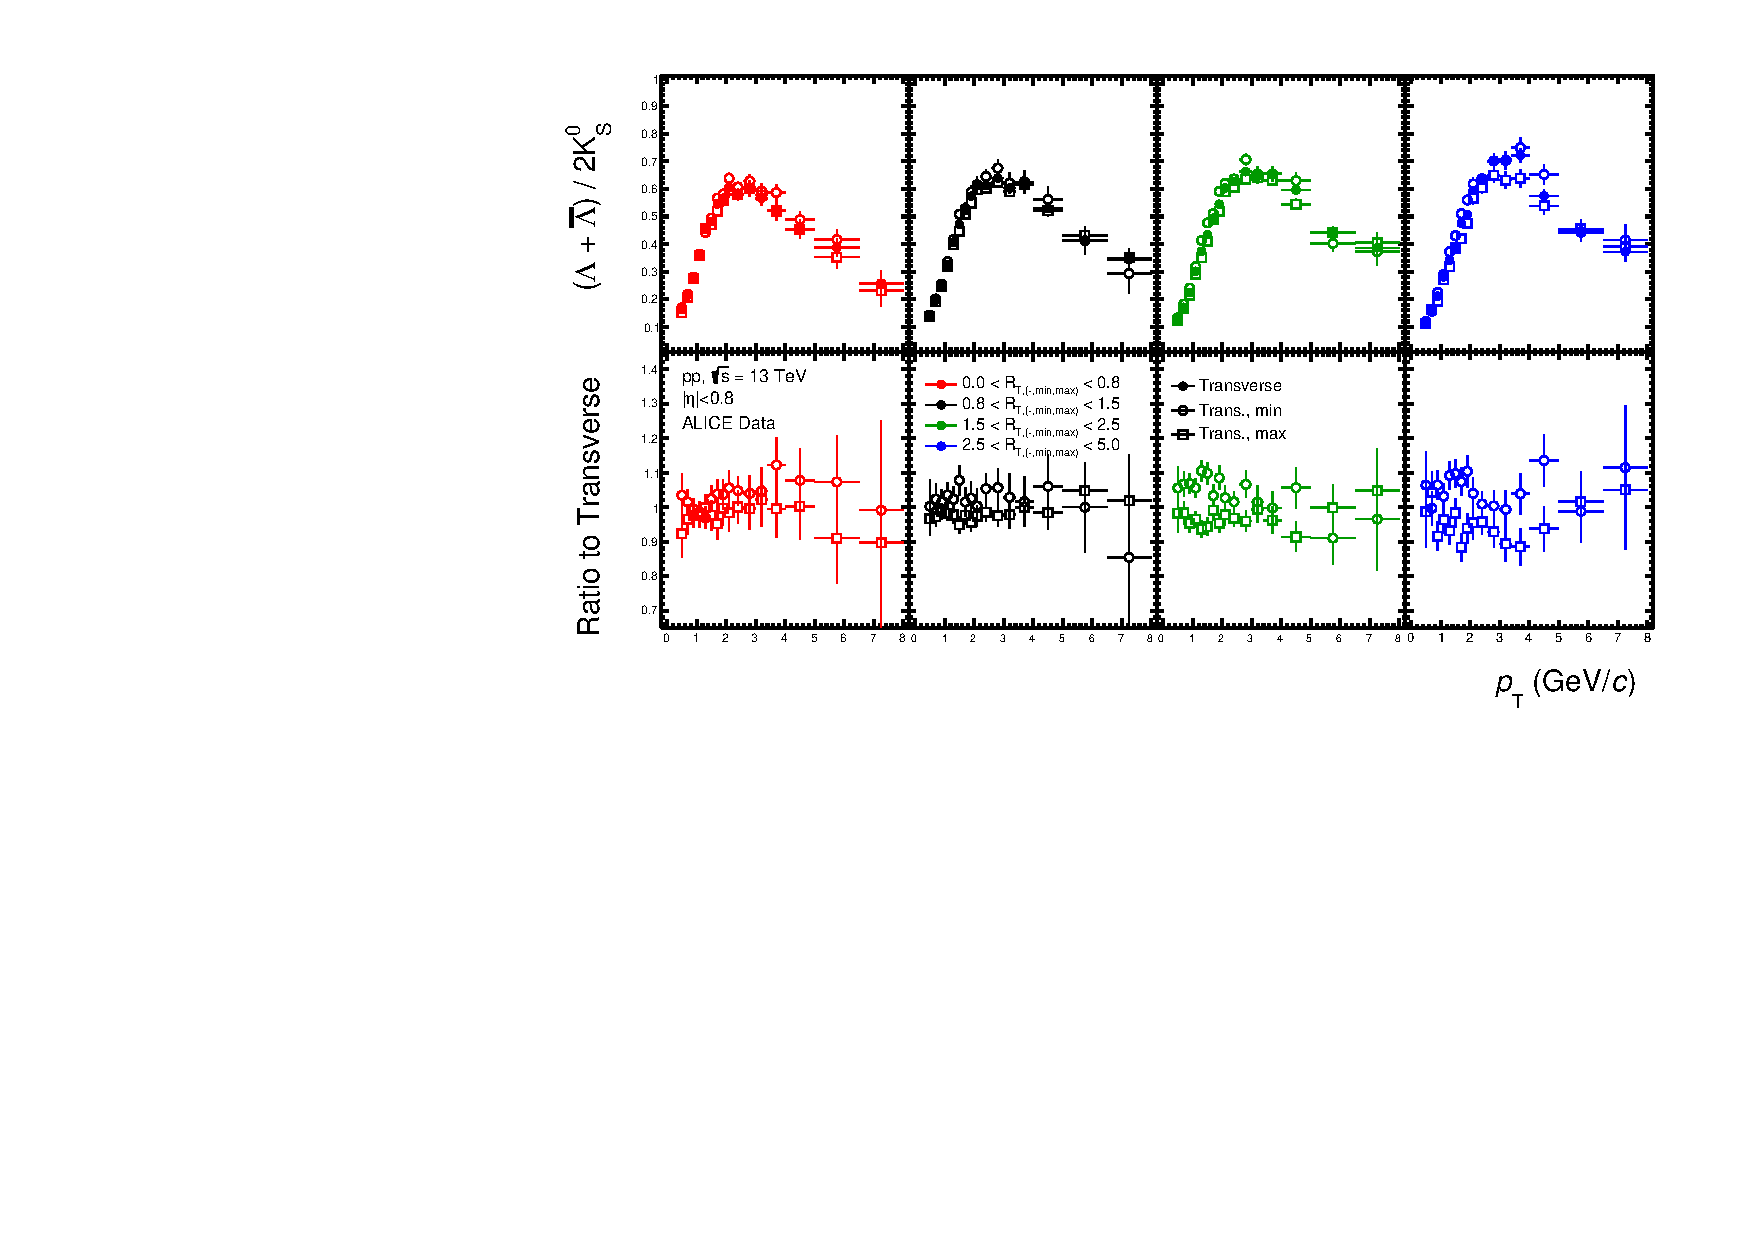
\includegraphics[width=.990\textwidth]{\imgpath/PtvRt_LtoK_Reg_K0s.pdf}}\\
\caption{TBA.}
\label{fig:rt:LtoKreg}
\end{figure}


\section{Integrated yields}

TBA

\begin{figure}%
\subfloat[][]{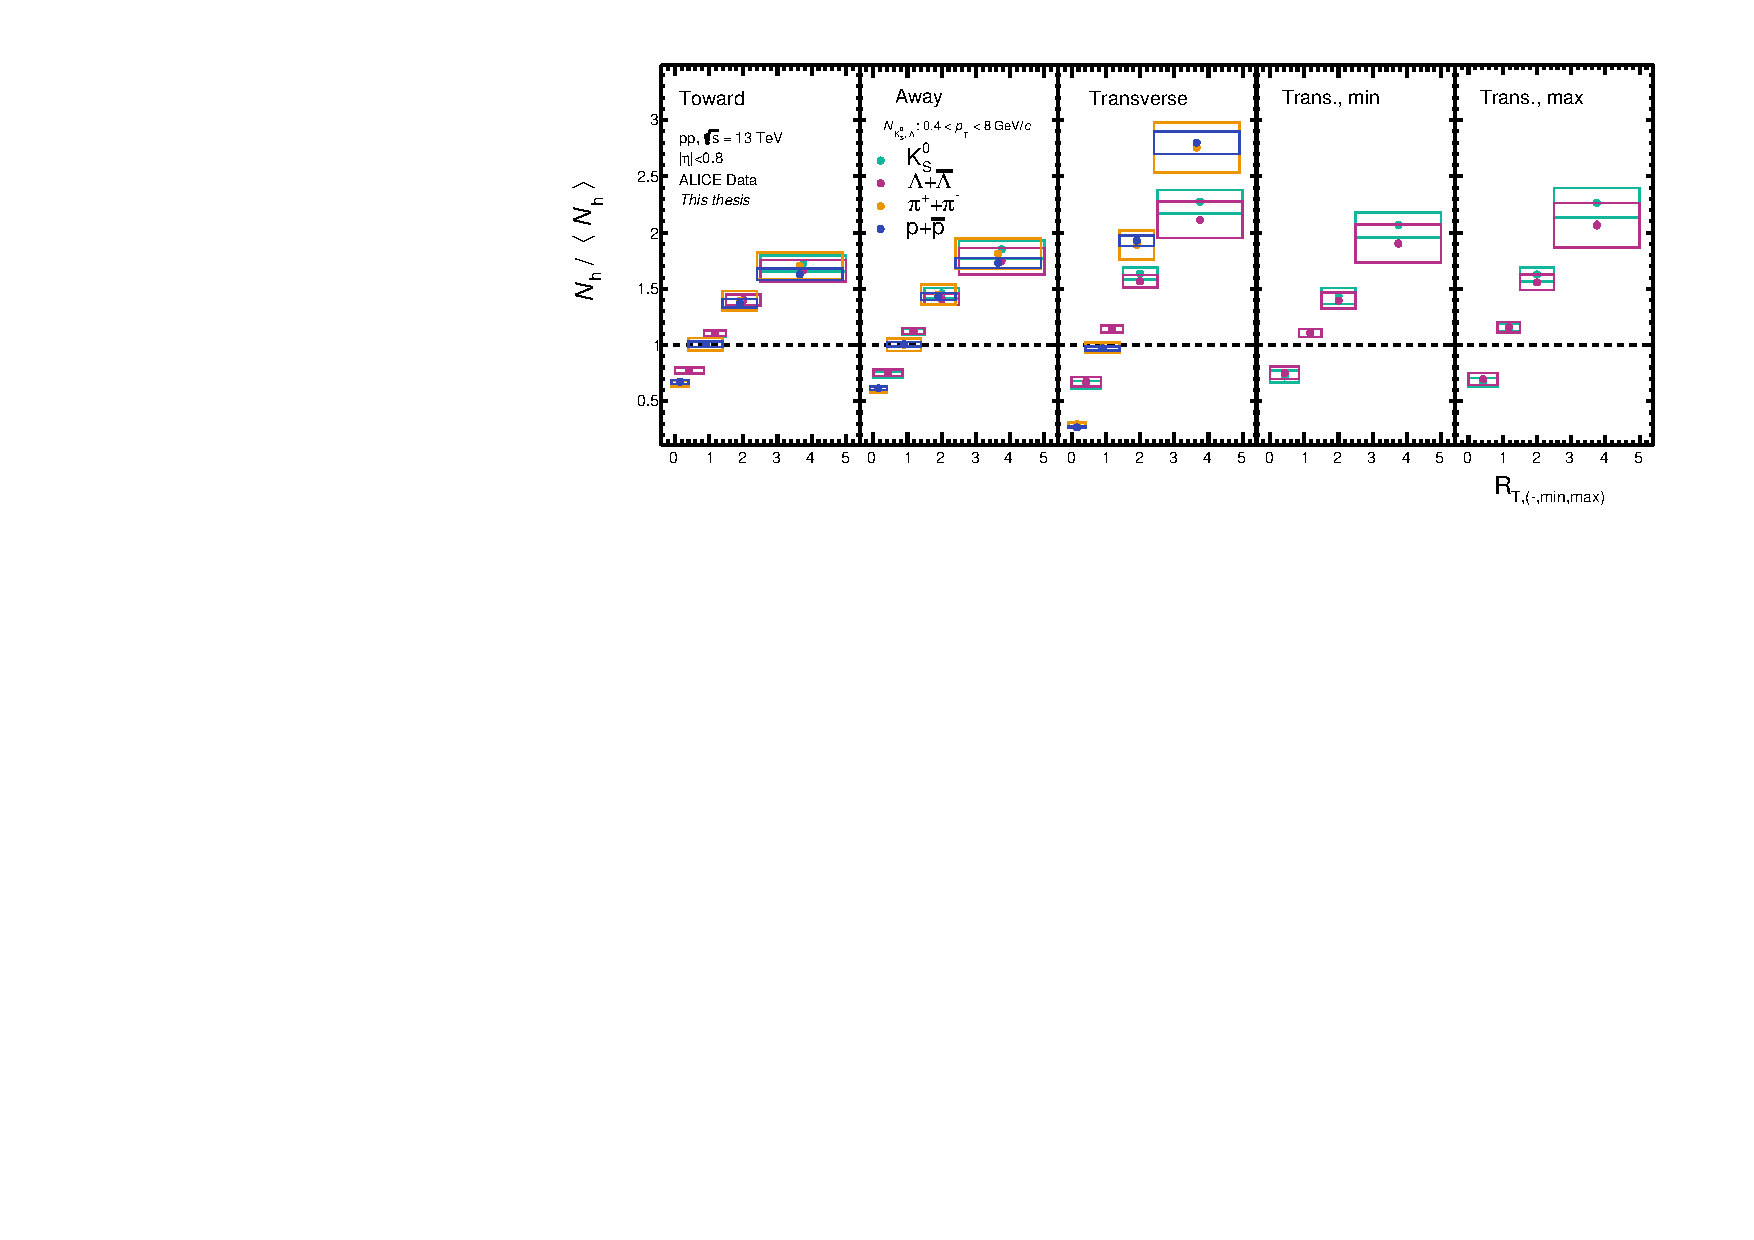
\includegraphics[width=.990\textwidth]{\imgpath/PtvRt_YieldPiKp_L.pdf}}\\
\subfloat[][]{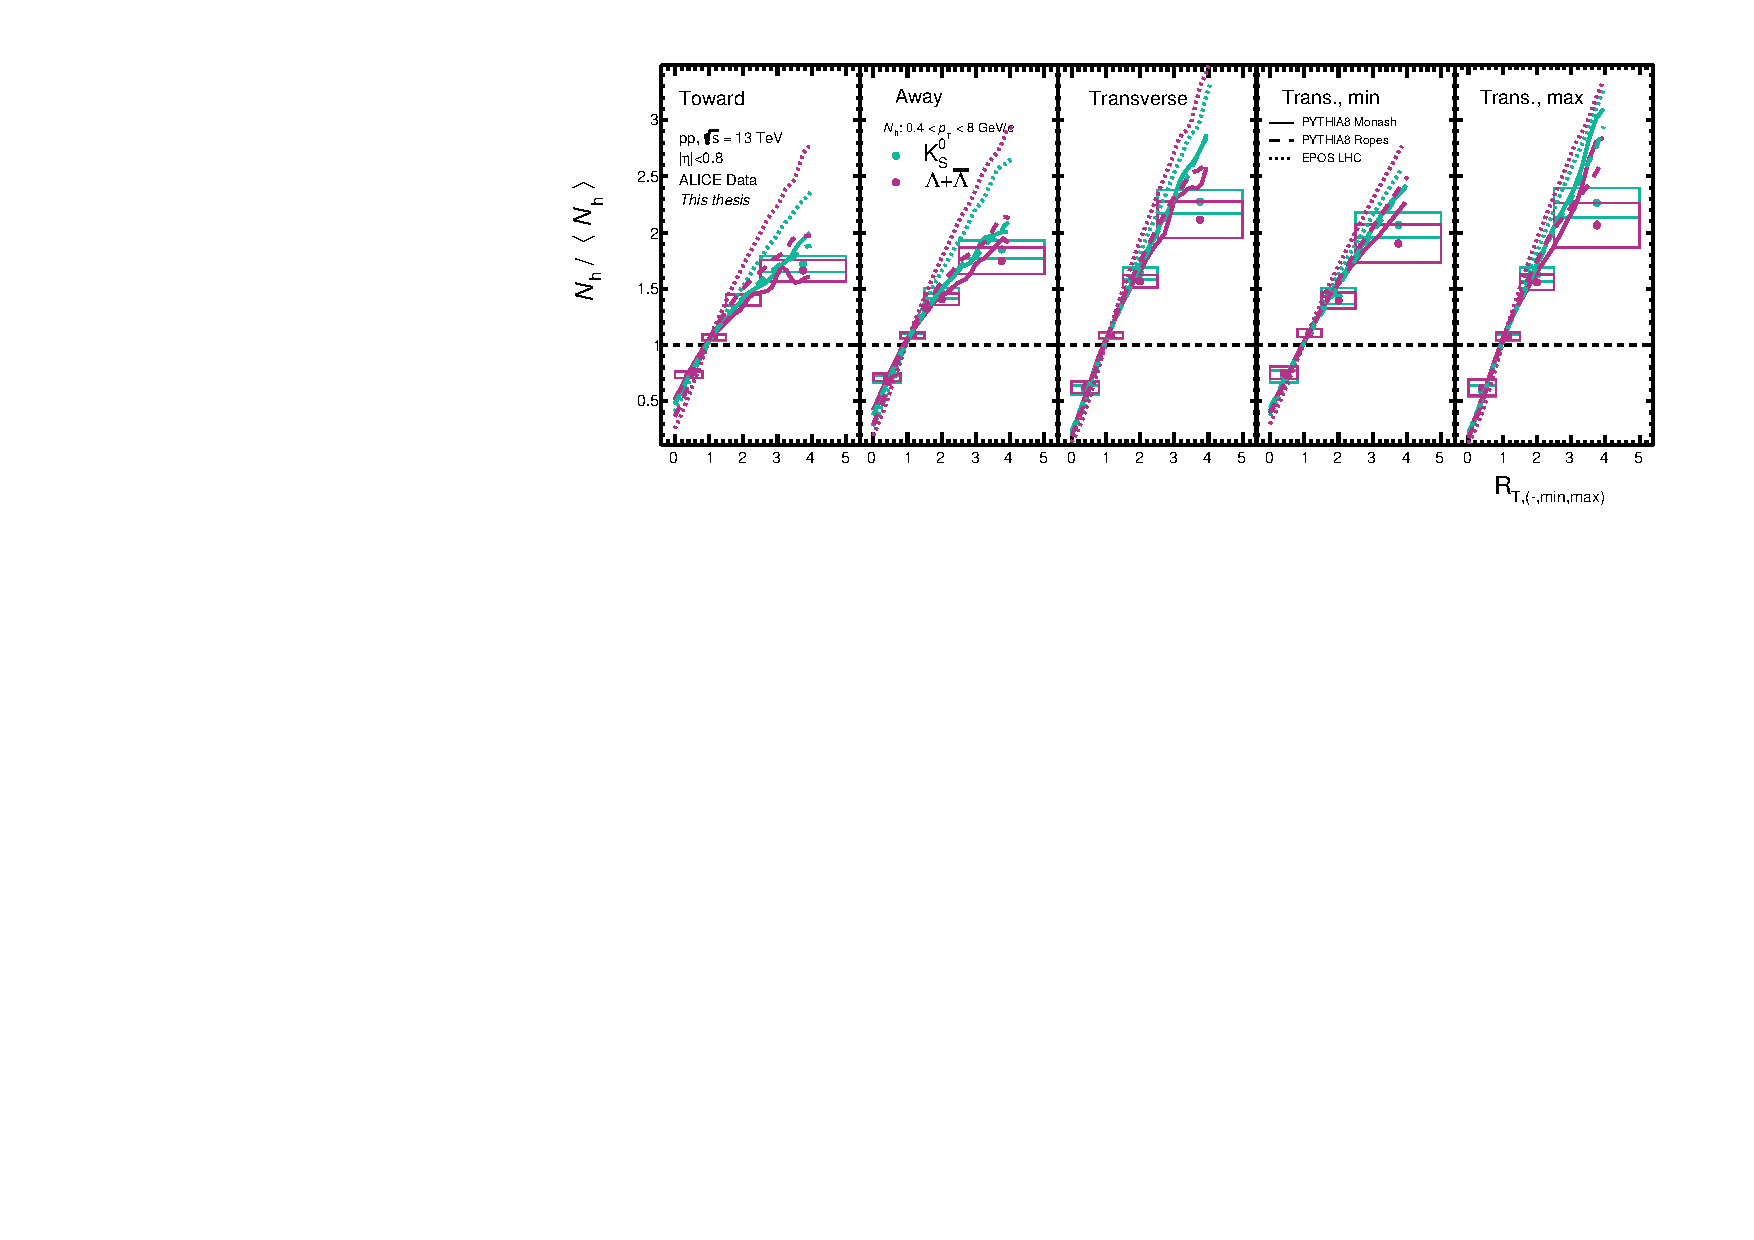
\includegraphics[width=.990\textwidth]{\imgpath/PtvRt_Yield_L.pdf}}\\
\caption{The measured and fully corrected \SOPT distributions for both \textbf{(a)} \NSPD 0--1\%, \textbf{(b)} 0--10\% and \textbf{(c)} \VOM 0--1\% . The curves represent different model prediction, where the shaded area represents the statistical uncertainty of the models.}
\label{fig:rt:yield}
\end{figure}




